% Seminario Girolamini 17 giugno 2020
%  temi:
% - recensio/raccolta e descrizione dei testimoni
% - collatio/esaminatio
% - costitutio/emendatio
% - pubblicazione/messa in pagina
%
% - Intro XML <https://www.tei-c.org/release/doc/tei-p5-doc/en/html/SG.html>
%
% - Intro TEI < https://books.openedition.org/oep/426 >
%
% - TEI Modulo 12 < https://www.tei-c.org/release/doc/tei-p5-doc/en/html/TC.html >
%
% - Tool di allineamento per la collazione:
%
% -- http://v-machine.org/documentation/
%
% -- https://collatex.net/
%
% -- http://www.juxtacommons.org/
%
% -- https://sada.uzi.uni-halle.de/
%
% -- medite
%
% -- tustep/TXSTEP
%
% -- http://evt.labcd.unipi.it/

% -- http://www.informatik.uni-leipzig.de:8080/BibleViz/

% ecdotica: resa grafica, messa in pagina
% -- https://ride.i-d-e.de/issues/issue-11/reledmac/
% -- https://tei-c.org/2014/06/10/tei-critical-edition-toolbox/
% -- http://teicat.huma-num.fr/index.php

\documentclass{beamer}
    
%    \usepackage[english]{babel}
    %\usepackage[latin1]{inputenc}
    %\usepackage[T1]{fontenc}

\mode<presentation>{
  \setbeamertemplate{background canvas}[vertical shading]
  \usetheme{Berkeley}
  \useoutertheme{himinfolines}
}
  
\usepackage{ucs}
\usepackage[utf8]{inputenc}
\usepackage[english,polutonikogreek,italian,UKenglish,british]{babel}
\usepackage{graphicx}
\usepackage{colortbl}
\usepackage{multicol}
\usepackage{ulem}
\usepackage{verbatim}
\usepackage{alltt}
\usepackage{ccicons}
\usepackage{MnSymbol,wasysym}
\usepackage{tikzsymbols}
\usepackage{textcomp}
\usepackage{xmpincl}

\usepackage{parskip}
\setcounter{nframes}{250}
\setcounter{nframe}{1}
\setbeamercovered{dynamic}
\newenvironment{grcenv}{\begin{otherlanguage}{greek}}{\end{otherlanguage}}
\newcommand{\g}[1]{\textgreek{#1}}
\definecolor{darkgreen}{rgb}{0,0.5,0}
\definecolor{darkblue}{rgb}{0,0,0.5}
\definecolor{grey}{rgb}{0.5,0.5,0.5}
\setcounter{tocdepth}{5}

\makeatletter

\makeatother
%\includexmp{LicencesAndLicensing}

%frame00 metadata
	\title{Dalla Recensio all'Emendatio Digitale}
	\author[A.M. Del Grosso]{Angelo Mario Del Grosso}
	%\institute{}
	%\institute{\texttt{angelo.delgrosso@ilc.cnr.it} \\\bigskip\textit{CNR-ILC} \\\bigskip\url{http://ilc.cnr.it/}}
    \institute{\textit{CNR-ILC}\\\texttt{\url{http://ilc.cnr.it/}}\\\texttt{angelo.delgrosso@ilc.cnr.it} \\\bigskip\textbf{Teoria, Prassi e Strumenti}\\\textit{(Tecnologia informatica applicata alle scienze filologiche e librarie)}}
    \date{Istituto di Linguistica Computazionale ``A. Zampolli'', \today}
    \AtBeginSection[]{
    \begin{frame}<beamer>
    \addtocounter{nframe}{1}
    \footnotesize
    \frametitle{Progress status}
    \tableofcontents[currentsection,hideothersubsections]
    \end{frame}
    }

\begin{document}

\begin{frame}
	\maketitle
\end{frame}

\begin{frame}
	\frametitle{Argomenti trattati}
	\tableofcontents
\end{frame}

\section{Introduzione personale}

\begin{frame}
	\frametitle{Di cosa mi occupo}
	\addtocounter{nframe}{1}

	\begin{block}{Filologia Digitale e Computazionale}
		Attività di ricerca per lo sviluppo di sistemi di linguistica e filologia digitale e computazionale volti alla produzione, rappresentazione, analisi, fruizione e interrogazione di testi di tradizione medievale, a stampa e di autori moderni e contemporanei.
	\end{block}

\end{frame}

\begin{frame}
	\frametitle{Profilo professionale e di ricerca}
	\addtocounter{nframe}{1}

	\begin{block}{In sintesi}
		\begin{center}
			Ingegnere Informatico prestato alla filologia computazionale
		\end{center}
	\end{block}

	\begin{center}
		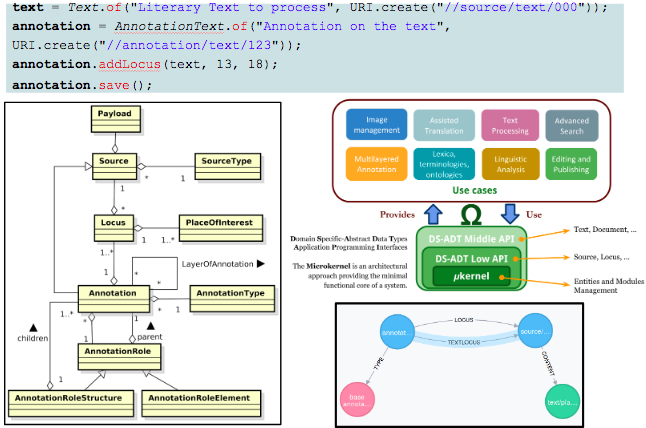
\includegraphics[width=.7\textwidth]{imgs/InfrastructureForTextualScholarship.png}
	\end{center}

\end{frame}

% \begin{frame}
% 	\frametitle{Temi del seminario}
% 	\addtocounter{nframe}{1}

% 	\begin{itemize}
% 		\item Filologia del testo 
% 		\begin{itemize}
% 			\item disciplina storica (insieme di discipline) dedicata al recupero/ricostruzione di un'opera - per lo più letteraria - e allo studio critico delle sue testimonianze condotto con metodo scientifico.
% 		\end{itemize}
% 		\item Metodo di Lachman
% 		\item Apparato Critico
% 		\begin{itemize}
% 			\item Apparato critico: nella edizione critica di un testo, l'apparato critico è il luogo (che può essere: a piè di pagina, in appendice al testo oppure dopo la nota al testo) in cui l'editore accoglie - a volte discutendolo (e comunque offrendo la possibilità di verifica del suo lavoro critico) - il complesso delle annotazioni, correzioni e varianti portate dalla tradizione e da lui giudicate erronee (o non meritevoli di essere accolte come lezione a testo).	
% 		\end{itemize}
% 		\item Collazione: collation is "to compare one text with another to discover textual variation"
% 		\item 
% 		\item 
% 	\end{itemize}

% \end{frame}

% Apparato critico negativo: l'apparato negativo o implicito non riporta la lezione a testo ma solo la lezione o le lezioni non accolte dell'altro o degli altri testimoni rappresentati con sigle distintive. Sta al lettore identificare nel testo la lezione corrispondente.
%Apparato critico positivo: l'apparato positivo o esplicito riporta la lezione a testo (in genere solo la prima e l'ultima parola di brani lunghi) non di rado delimitata da una parentesi quadra ( ] ), seguita dalla lezione o lezioni dell'altro o degli altri testimoni rappresentati con sigle distintive.

% \begin{frame}
% 	\frametitle{Temi del seminario}
% 	\addtocounter{nframe}{1}

% 	\begin{itemize}
% 		\item Codifica del testo 
% 		\begin{itemize}
% 			\item Rappresentazione formale con tecnologia digitale
% 			\item Livello di rappresentazione dei caratteri
% 			\item Livello di rappresentazione della struttura e dei fenomeni testuali
% 		\end{itemize}
% 	\end{itemize}

% \end{frame}

\begin{frame}
	\frametitle{Temi del seminario}
	\addtocounter{nframe}{1}

	\begin{center}
		
\includegraphics[width=.5\textwidth]{imgs/tei-r.pdf}
	\end{center}

\end{frame}

\begin{frame}
	\frametitle{Obiettivo del seminario}
	\addtocounter{nframe}{1}

	\begin{block}{approfondiremo}
		Tecniche per la rappresentazione digitale di edizioni critiche adottando le specifiche e le linee guida della \textit{Text Encoding Initiative} implementate adottando l'eXtensible Markup Language (\textit{TEI-XML}).
	\end{block}
	\begin{block}{approfondiremo}
		Strumenti per la collazione automatica e la pubblicazione di edizioni critiche digitali
	\end{block}

\end{frame}

% \begin{frame}
%     \frametitle{Perché è importante la codifica dei testi}
%     \framesubtitle{Motivazioni pratiche}
%     \addtocounter{nframe}{1}
    
%     \begin{block}{Perché codificare i testi}
%         Per rendere disponibile l'immenso patrimonio testuale tramite l'uso di sistemi digitali e computazionali è necessario effettuare una trasposizione/transcodifica\textsuperscript{*} dei testi dal loro supporto originario verso il nuovo supporto elettronico (\textit{Machine Readable Form} and \textit{Machine Actionable Form}).
%     \end{block}

%     \begin{center}
%         * \textit{procedimento di conversione dei dati codificati secondo un sistema verso un sistema diverso}
%     \end{center}

% \end{frame}

% \begin{frame}
% 	\frametitle{Elementi di Codifica dei Caratteri}
% 	\framesubtitle{Definizioni}
% 	\addtocounter{nframe}{1}

% 	\begin{block}{Rappresentare il testo in formato digitale}
% 		L’adozione di metodologie e tecnologie informatiche per il trattamento di documenti testuali richiede in primo luogo la disponibilità di un'adeguato sistema di rappresentazione digitale dei dati - presenti nella risorsa originale - e conseguentemente un formalismo adatto a tale rappresentazione.
% 	\end{block}

% \end{frame}

% \begin{frame}
% 	\frametitle{Elementi di Codifica del testo}
% 	\framesubtitle{Formalismi}
% 	\addtocounter{nframe}{1}

% 	\begin{block}{Formati e formalismi di codifica}

% 		Ogni pezzo di informazione aggiunta ad un testo grezzo attraverso l'inserimento di dati metatestuali (markup, annotazione, codifica), constituisce il risultato di una analisi e di una interpretazione che è stata condotta (da un umano o da una macchina) al fine di esplicitare e rappresentare nel modo più accurato e completo possibile le informazioni da veicolare attraverso il formato digitale prescelto (anche in modo incrementale).


% 	\end{block}

% \end{frame}

\section{Panoramica Text Encoding Initiative}
\begin{frame}
	\frametitle{Markup language e XML}
	\framesubtitle{soluzione corrente per la codifica dei testi}
	\addtocounter{nframe}{1}

	\begin{block}{TEI-XML}
		Considerato ad oggi lo standard de facto per la codifica dei testi è lo schema XML messo a punto dalla Text Encoding Initiative (TEI-XML).
	\end{block}

\end{frame}

\begin{frame}
    \frametitle{Introduction}
    \addtocounter{nframe}{1}
    
    \begin{center}
        \includegraphics[width=.95\textwidth]{imgs/1.png}
    \end{center}

\end{frame}

 


\section{Panoramica eXtensible Markup Language}
\begin{frame}
	\frametitle{I linguaggi di codifica}
	\framesubtitle{introduzione}
	\addtocounter{nframe}{1}

	\begin{block}{Definizione di codifica digitale del testo}
		Per \textbf{codifica} digitale dei testi intendiamo la \textit{rappresentazione formale} di un \textbf{testo} ad un qualche livello descrittivo, su di un supporto digitale, in un formato utilizzabile da un elaboratore (\textit{Machine Readable Form}) mediante un opportuno \textbf{linguaggio informatico} (F. Ciotti).
	\end{block}

\end{frame}

\begin{frame}
	\frametitle{Markup language e XML}
	\framesubtitle{soluzione corrente per la codifica dei testi}
	\addtocounter{nframe}{1}

	\begin{block}{XML per la descrizione e la codifica}
		Ad oggi la soluzione considerata ottimale per una corretta rappresentazione del testo è l'adozione dei markup language descrittivi basati su XML.
	\end{block}

\end{frame}

\begin{frame}
	\frametitle{I linguaggi di codifica}
	\framesubtitle{Linguaggi di marcatura}
	\addtocounter{nframe}{1}

	\begin{block}{Il markup}
		Il termine \textbf{markup} è stato utilizzato in passato per denotare i \textbf{segni grafici} che accompagnavano un testo apposti sul documento per \textbf{indicare correzioni o modalità grafiche di stampa}.
	\end{block}

\end{frame}

\begin{frame}
	\frametitle{I linguaggi di codifica}
	\framesubtitle{Linguaggi di marcatura}
	\addtocounter{nframe}{1}

	\begin{center}
		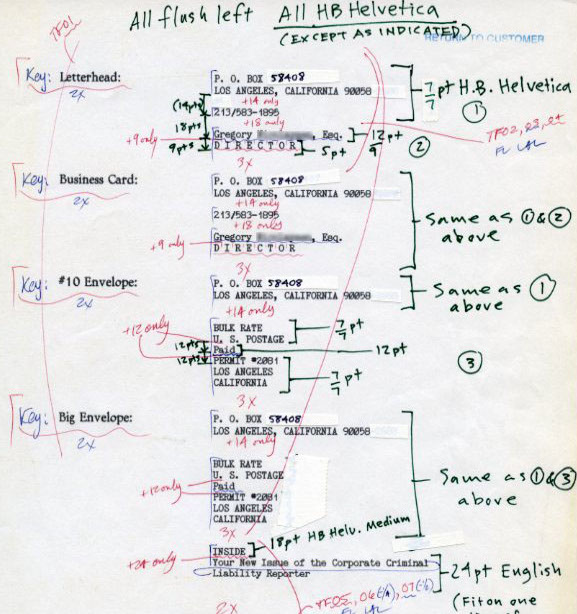
\includegraphics[width=.6\textwidth]{imgs/xml-markup001.jpg}
	\end{center}

\end{frame}

\begin{frame}
	\frametitle{I linguaggi di codifica}
	\framesubtitle{Linguaggi di marcatura}
	\addtocounter{nframe}{1}

	\begin{center}
		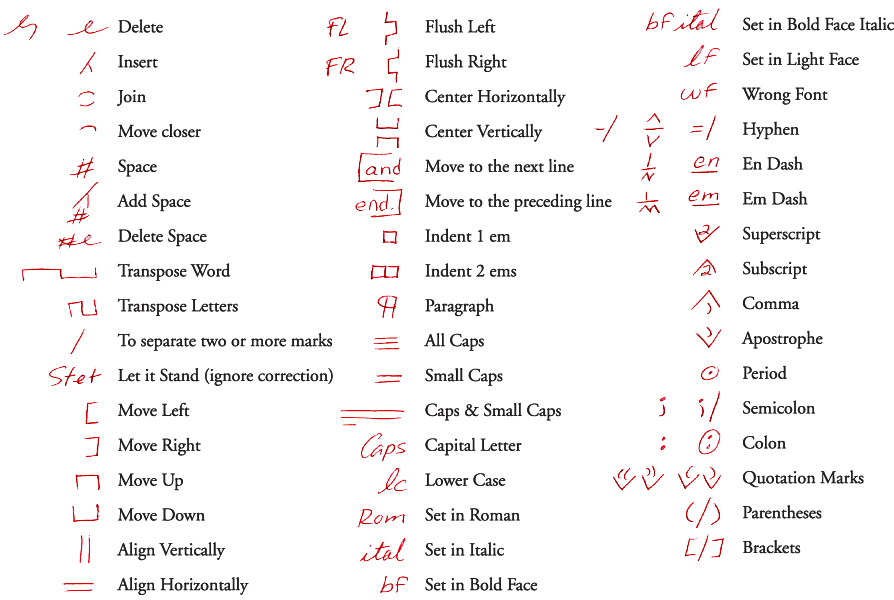
\includegraphics[width=.9\textwidth]{imgs/xml-MarkupConvention.png}
	\end{center}

\end{frame}

\begin{frame}
	\frametitle{I linguaggi di codifica}
	\framesubtitle{Linguaggi di marcatura}
	\addtocounter{nframe}{1}

	\begin{block}{Il markup}
		La codifica con linguaggi di marcatura (markup) è in sostanza \textbf{un insieme di convenzioni}, rese attraverso specifiche \textbf{sequenze di caratteri, etichette, codici}, (detti \textit{tags}) \textbf{intercalati nel testo} per permettere agli elaboratori elettronici di distinguere le varie parti di un documento.
	\end{block}

	\begin{block}{Il markup formale}
		Un linguaggio di markup è un \textbf{sistema formale} per \textit{scambiare} e \textit{pubblicare} informazioni in \textbf{formato testo in modo strutturato}.
	\end{block}


\end{frame}

%slide relative ad introdurre gli elementi di XML

% prendere da libro XML in amazon e XML visual quick view
% inserire qualche nota sul namespace anche preso dal libro xsd da pag 26 
% riprendere qualche slide dall slide Del Turco; e dalle slide Fiormonte-Ciotti-Silvi-XML-corso-2014.pdf
% http://filologiadigitale-verona.it/wp-content/uploads/2014/10/Fiormonte-Ciotti-Silvi-XML-corso-2014.pdf
% Slide Chiara di Pietro

% IDE/Editor comes with a nice XML/XSD editor. It has a number of features that makes schema writing lot easier. Intellisense, auto-completion, real-time syntax checks, etc., are a few of those features.

\begin{frame}
	\frametitle{Fondamenti XML}
	\framesubtitle{eXtensible Markup Language}
	\addtocounter{nframe}{1}

	
	\begin{block} {eXtensible Markup Language}
		L'\textit{XML è un meta-linguaggio}, usato per \textit{create linguaggi di marcatura} (detti \textbf{vocabolari}).
	\end{block}
\end{frame}

\begin{frame}
	\frametitle{Fondamenti XML}
	\framesubtitle{eXtensible Markup Language}
	\addtocounter{nframe}{1}

	\begin{block}{XML come meta-linguaggio}
		XML, \textit{eXtensible Markup Language}, \textbf{è un insieme di regole} per definire linguaggi di marcatura personalizzati e personalizzabili (\textit{custom-built vocabolaries}).
	\end{block}

	\begin{block} {Applicazioni XML}
		XML è nato per \textbf{strutturare}, \textbf{conservare} e \textbf{trasportare} informazioni.
		\\ I linguaggi di marcatura derivati da XML per strutturare e descrivere specifiche informazioni vengono chiamati \textit{XML applications} oltre che \textit{vocabolario XML}.
	\end{block}
\end{frame}

\begin{frame}
	\frametitle{Fondamenti XML}
	\framesubtitle{eXtensible Markup Language}
	\addtocounter{nframe}{1}

	\begin{block}{XML: eXtensible}
		XML è \textbf{estensibile}: è pensato per essere \textit{modificato} ed \textit{esteso} al fine di soddisfare le varie necessità di rappresentazione dell'informazione.
		\textbf{XML non contempla un vocabolario predefinito!}
	\end{block}

	\begin{block} {XML: standard W3C}
		XML è sviluppato e \textbf{manutenuto dal W3C} (World Wide Web Consortium), il quale sviluppa \textit{protocolli} e \textit{standard} riconosciuti dalla comunità scientifica e tecnica al fine di \textbf{condividere informazioni sul Web}.
	\end{block}
\end{frame}

\begin{frame}
	\frametitle{Fondamenti XML}
	\framesubtitle{eXtensible Markup Language}
	\addtocounter{nframe}{1}

	\begin{block}{XML: riassumendo}
		XML, eXtensible Markup Language, deriva da SGML ed 
		è una \textbf{specificazione}, un \textbf{formalismo}, per \textit{strutturare}, \textit{conservare} e \textit{scambiare} informazioni in formato machine readable (\textit{digitale}).
	\end{block}

	\begin{block}{XML: riassumendo}
		XML è anche una specificazione per \textbf{descrivere la struttura dell'informazione} seguendo un \textbf{modello dei dati gerarchico}.
		\\ XML è simile ad HTML, ma a differenza di questo non ha etichette predefinite.
	\end{block}

\end{frame}


\begin{frame}
	\frametitle{Fondamenti XML}
	\framesubtitle{eXtensible Markup Language}
	\addtocounter{nframe}{1}

	\begin{center}
		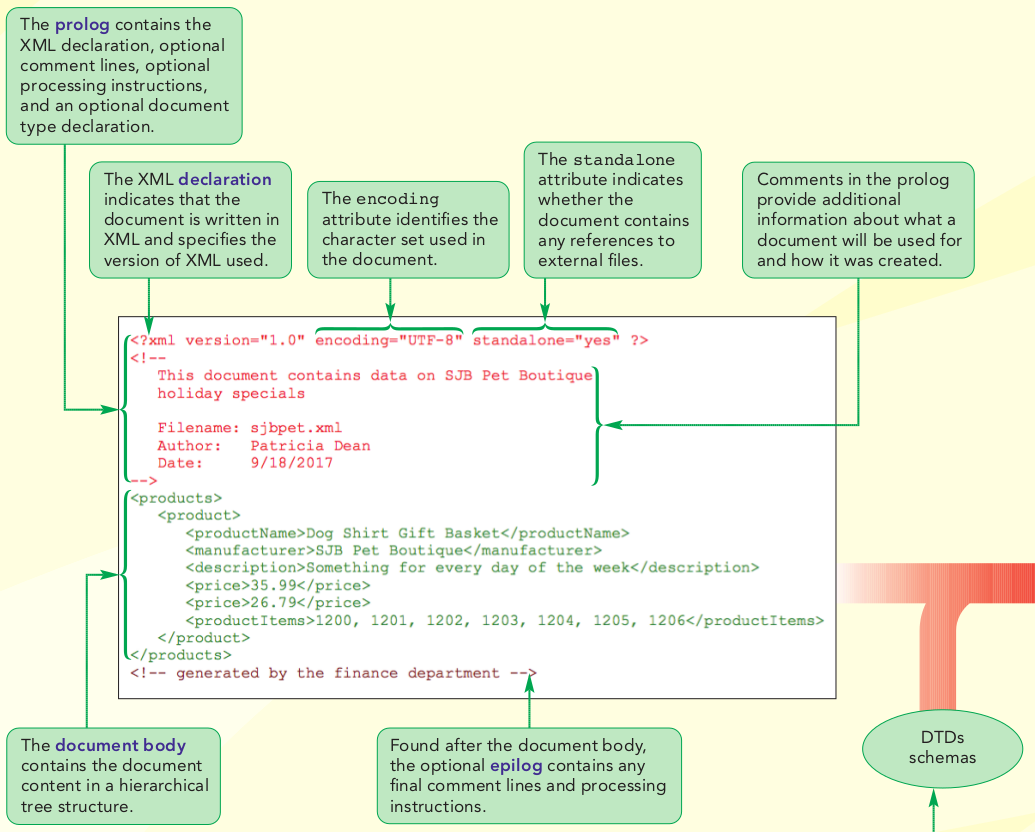
\includegraphics[width=.8\textwidth]{imgs/xml-intro-doc-xml.png}
	\end{center}

	\begin{tiny}\textit{immagine dal libro New Perspectives on XML, 3rd Edition}\end{tiny}

\end{frame}


%The syntax rules of XML are easy to learn and easy to use
\begin{frame}
	\frametitle{Fondamenti XML}
	\framesubtitle{eXtensible Markup Language: regole sintattiche}
	\addtocounter{nframe}{1}

	\begin{itemize}

		\item Ciascun elemento XML deve avere un tag di chiusura.
			%Every XML element must have a closing tag.
		      %Every element must have a closing tag. A self-closing tag is permitted.

		\item I tag XML sono \textit{case sensitive}.
			%XML tags are case sensitive.
		      % Opening and closing tags (or start and end tags) must be ­written with the same case.

		\item Gli elementi XML devono essere annidati in modo rigoroso.
			%XML elements must be ­properly nested.
		      %All elements can have child (sub) elements. Child elements must be in pairs and be correctly nested within their respective parent element.

		\item Tutti i documenti XML deveno avere un elemento radice (root) che contiene tutti gli altri elementi opportunamente annidati.
			%Every XML document must have a root element.
		      %Every XML document must contain a single tag pair that defines the root element. All other elements must be nested within the root element.

		\item Gli elementi XML possono avere attributi con stile nome-valore.
		
	\end{itemize}

\end{frame}


%The syntax rules of XML are easy to learn and easy to use 2
\begin{frame}
	\frametitle{Fondamenti XML}
	\framesubtitle{eXtensible Markup Language: regole sintattiche cont.}
	\addtocounter{nframe}{1}

	\begin{itemize}
		\item Un attributo all'interno dell'elemento può apparire una sola volta
		
		\item Il valore degli attributi è una stringa e deve essere inserita tra apici
			%XML elements can have attributes in name-value pairs.
		      %Each attribute name within the same element can occur only once.% Each attribute value must be quoted.

		\item Esistono alcuni caratteri speciali che non possono essere usati. 
			%Some characters have a ­special meaning in XML.
		      %The use of certain characters is restricted. If these characters are needed, entity references or character references may be used. References always begin with the character “&” (which is ­specially reserved) and end with the character “;”.

		      %XML allows for comments. 
		\item I commenti non possono essere inseriti prima della dichiarazione XML e non possono essere annidati.
			%Comments cannot occur prior to the XML Declaration. Comments cannot be nested.

	\end{itemize}

\end{frame}

\begin{frame}
	\frametitle{Fondamenti XML}
	\framesubtitle{eXtensible Markup Language}
	\addtocounter{nframe}{1}

	\begin{block}{Manutenibilità}
		Data la semplicità delle regole e della sintassi XML incentrata sulla memorizzazione e scambio dei dati, la struttura generale di un documento XML è semplice sia dal punto di vista della progettazione sia dal punto di vista della manutenibilità.
	\end{block}

\end{frame}

\begin{frame}
	\frametitle{Fondamenti XML}
	\framesubtitle{eXtensible Markup Language}
	\addtocounter{nframe}{1}

	\begin{block}{XML vista ad albero}
		XML ha un modello dei dati gerarchico e può quindi essere visto come un albero ordinato.
		\\Per questo motivo le informazioni sono rappresentate in modo ottimale se sono gerarchiche e sequenziali.
	\end{block}

\end{frame}


\begin{frame}
	\frametitle{Fondamenti XML}
	\framesubtitle{eXtensible Markup Language: vista ad albero}
	\addtocounter{nframe}{1}

	\begin{center}
		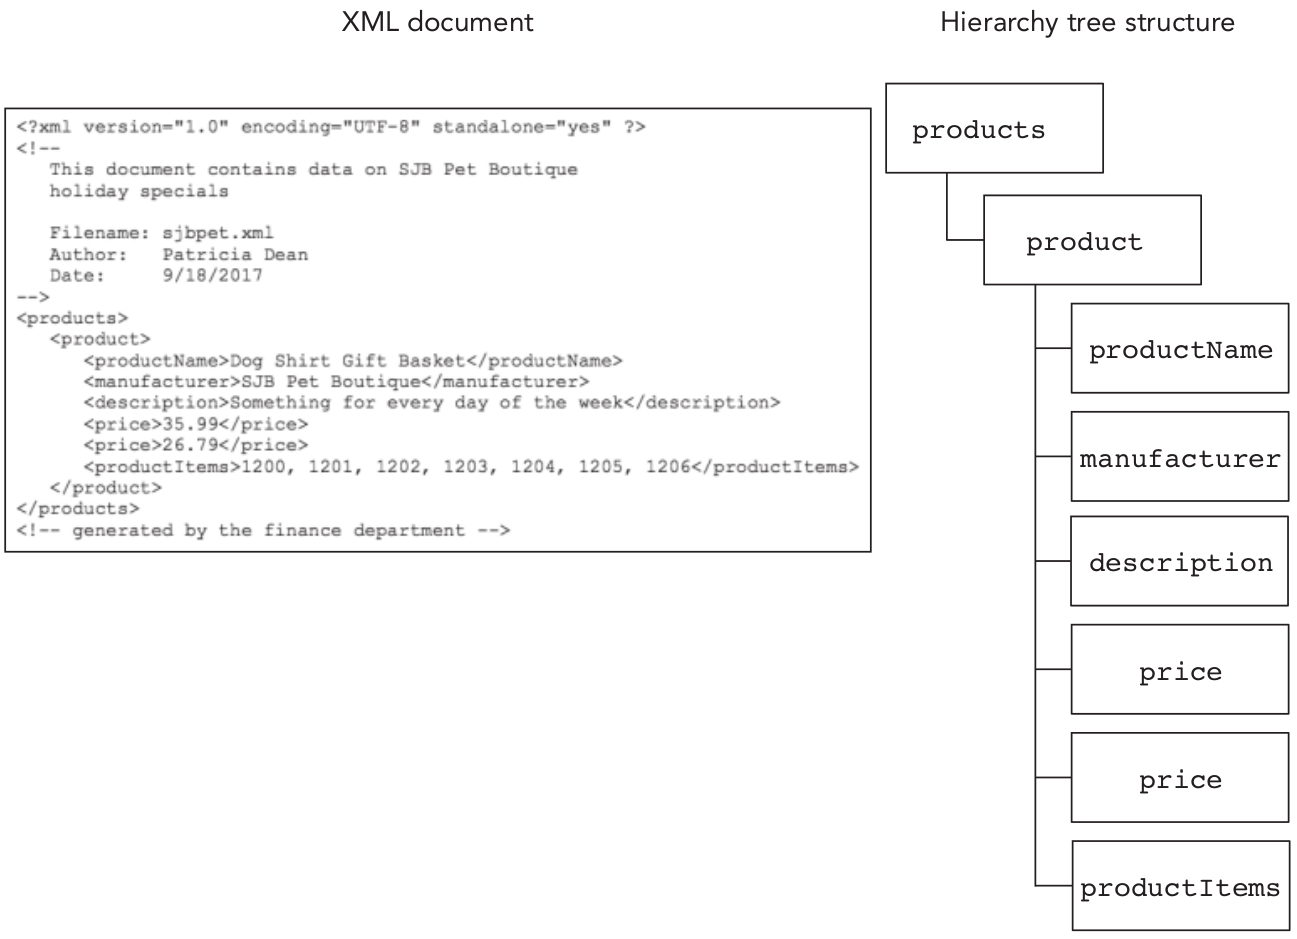
\includegraphics[width=.9\textwidth]{imgs/XML-TreeStructure.png}
	\end{center}

\begin{tiny}\textit{immagine dal libro New Perspectives on XML, 3rd Edition}\end{tiny}

\end{frame}

\begin{frame}
	\frametitle{Fondamenti XML}
	\framesubtitle{eXtensible Markup Language}
	\addtocounter{nframe}{1}

	\begin{block}{TEI-XML vocabulary}
		Al fine di soddisfare i \textbf{requisiti degli studiosi del testo} il \textit{vocabolario TEI-XML} è stato sviluppato nel corso degli ultimi decenni con lo scopo e l'obiettivo di \textit{permettere la codifica di qualsiasi informazione testuale}.
	\end{block}
	
	\textit{Un vocabolario XML è un insieme di tag XML sviluppato per una particolare esigenza di codifica}

\end{frame}


\begin{frame}
	\frametitle{Fondamenti XML}
	\framesubtitle{eXtensible Markup Language: Esempio TEI}
	\addtocounter{nframe}{1}

	\begin{center}
		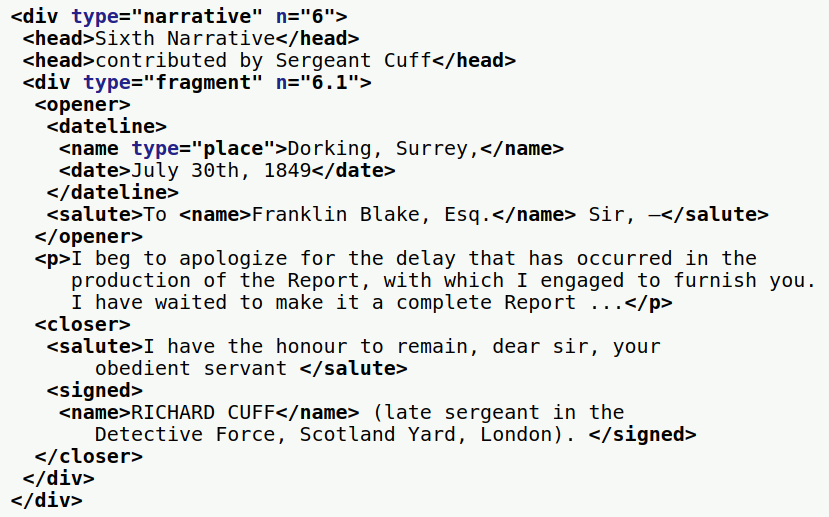
\includegraphics[width=.9\textwidth]{imgs/xml-TEI-Example.png}
	\end{center}

	\begin{tiny}
        \textit{immagine dal sito TEI Guide Lines}
    \end{tiny}

\end{frame}


\begin{frame}
	\frametitle{Fondamenti XML}
	\framesubtitle{eXtensible Markup Language}
	\addtocounter{nframe}{1}

	\begin{block}{Documento ben formato (well-formed)}
		Un documento XML deve essere \textbf{ben formato} (\textit{well-formed},cioè non deve contenere \textbf{errori sintattici} e deve soddisfare le \textbf{regole generali della specifica}.
	\end{block}
	\textit{Un documento non ben formato non può essere letto dalle applicazioni che elaborano codice XML}.

\end{frame}


\begin{frame}
	\frametitle{Fondamenti XML}
	\framesubtitle{eXtensible Markup Language}
	\addtocounter{nframe}{1}

	\begin{block}{Parti principali di un documento XML}
		Un documento XML consiste di tre parti:
		\begin{itemize}
			\item il prologo
			\item il corpo (body)
			\item l'epilogo
		\end{itemize}
	\end{block}

\end{frame}


\begin{frame}
	\frametitle{Fondamenti XML}
	\framesubtitle{eXtensible Markup Language: Esempio TEI}
	\addtocounter{nframe}{1}

	\begin{center}
		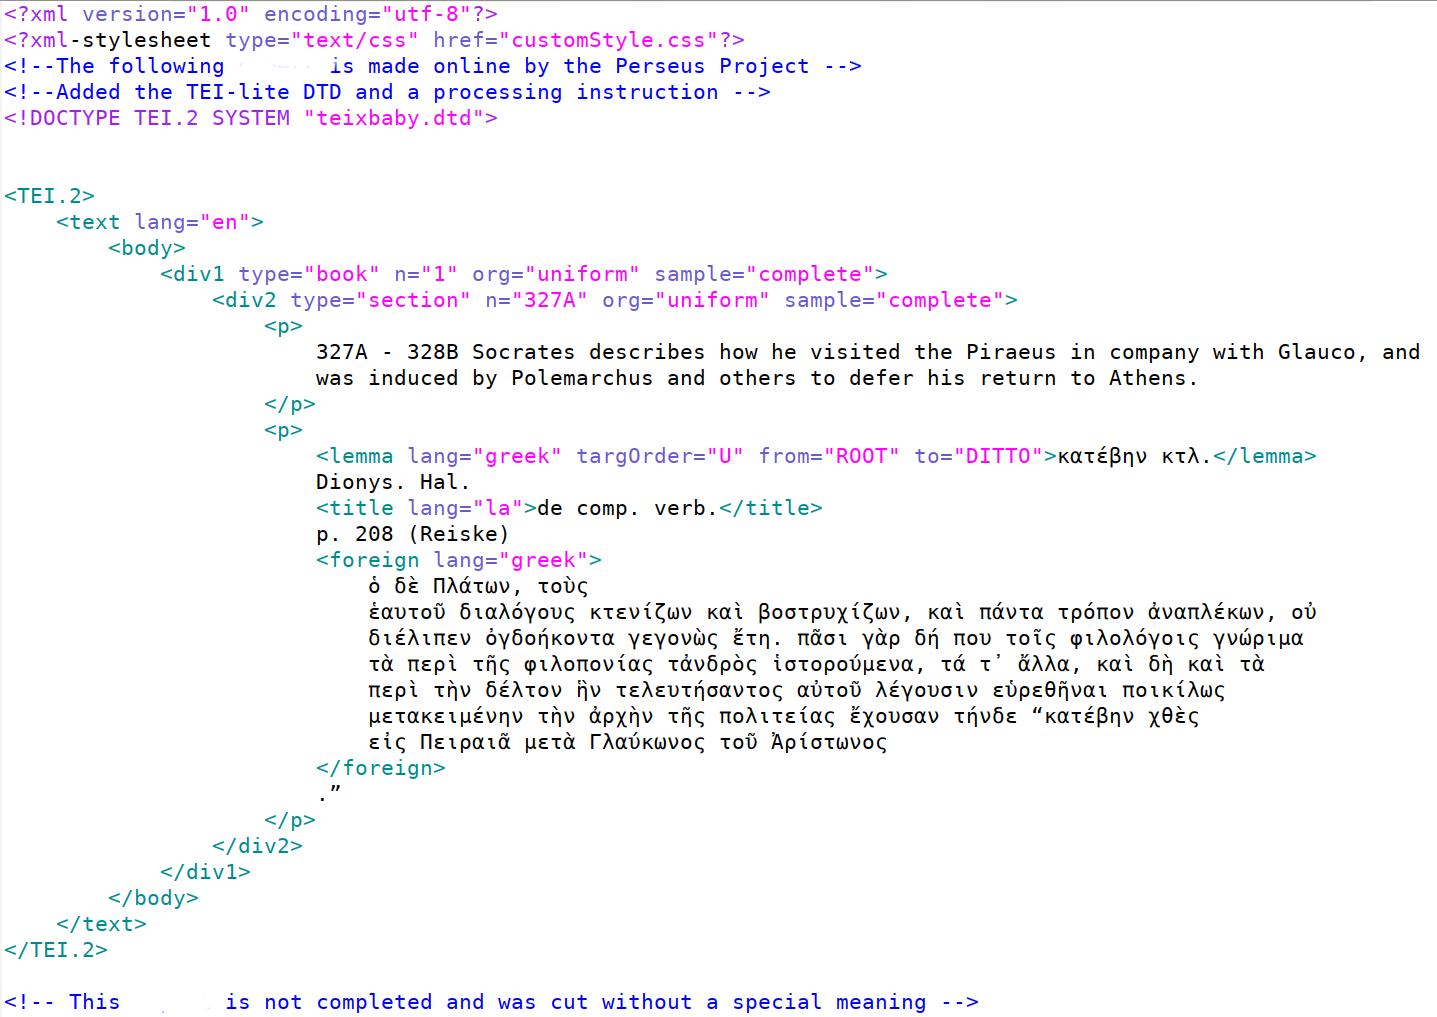
\includegraphics[width=0.95\textwidth]{imgs/xml-TEI-PerseusExample.png}
	\end{center}

\end{frame}


\begin{frame}
	\frametitle{Fondamenti XML}
	\framesubtitle{eXtensible Markup Language}
	\addtocounter{nframe}{1}

	\begin{block}{Documento XML: prologo}
		\begin{itemize}
			\item XML declaration (obbligatorio)
			\item Processing instructions (opzionale)
			\item Commenti (opzionale)
			\item Document type declaration (opzionale)
		\end{itemize}
        
        % XML declaration: indicates that the document is written in the XML language
        % Processing instructions (optional): provide additional instructions to be run by programs that read the XML document
        % Comment lines (optional): provide additional information about the document contents
        % Document type declaration (DTD) (optional): provides information about the rules used in the XML document’s vocabulary
	\end{block}

\end{frame}

\begin{frame}
	\frametitle{Fondamenti XML}
	\framesubtitle{eXtensible Markup Language}
	\addtocounter{nframe}{1}

	\begin{block}{Documento XML: corpo}
		Il corpo del documento XML segue immediatamente il prologo. Questa parte del documento contiene il contenuto vero e proprio in una \textbf{struttura ad albero ordinata}.
	\end{block}

	\begin{block}{Documento XML: epilogo}
		Opzionalmente, al corpo del documento XML segue un epilogo il quale può contenere commenti finali e processing instructions.
	\end{block}
	

\end{frame}

\begin{frame}
	\frametitle{Fondamenti XML}
	\framesubtitle{eXtensible Markup Language: Prologo}
	\addtocounter{nframe}{1}

	\begin{block}{XML declaration}
    \begin{center}\texttt{<?xml version=”version number” encoding=”encoding type” standalone=”yes|no” ?>}\end{center}
	\end{block}

\end{frame}

% Creating an XML Declaration
% • To create an XML declaration, enter the code
% <?xml ?>
% in the first line of an XML document.
% • To specify a version of XML to use, enter the code
% version=”version number”
% after the opening <?xml tag, where version number is either 1.0 or 1.1.
% • To specify a character encoding, enter the code
% encoding=”encoding type”
% after the version attribute-value pair, where encoding type identifies the ­character
% set used in the document.
% • To indicate whether the document is a standalone document, enter the code
% standalone=”yes|no”
% after the encoding attribute-value pair, where the value yes or no ­indicates whether
% access to external files will be needed when processing the document.

% \begin{frame}
% 	\frametitle{Fondamenti XML}
% 	\framesubtitle{eXtensible Markup Language: Prologo}
% 	\addtocounter{nframe}{1}

% 	\begin{block}{XML declaration: ERRORI}
% 	\begin{center}\texttt{<?XML VERSION=”1.0” ENCODING=”ISO-8859-1” STANDALONE=”YES” ?>}\end{center}
% 	\begin{center}\texttt{<?xml version=1.0 encoding=ISO-8859-1 standalone=yes ?>}\end{center}
% 	\begin{center}\texttt{<?xml version=”1.0” standalone=”yes” encoding=”ISO-8859-1” ?>}\end{center}
% 	\end{block}

% \end{frame}

\begin{frame}
	\frametitle{Fondamenti XML}
	\framesubtitle{eXtensible Markup Language: Prologo}
	\addtocounter{nframe}{1}

	\begin{block}{XML comments}
		I commenti XML vengono ignorati dai programmi che elaborano il documento.
		\\I commenti quindi non influenzano i contenuti e la struttura del documento.
	\end{block}

	\begin{block}{XML comments: sintassi}
	\begin{center}\texttt{
		<!-- il parser XML qui non entra -->
	}\end{center}
	\end{block}

	\textit{Un commento può occupare anche più righe}
	
\end{frame}

\begin{frame}
	\frametitle{Fondamenti XML}
	\framesubtitle{eXtensible Markup Language}
	\addtocounter{nframe}{1}

	\begin{center}
		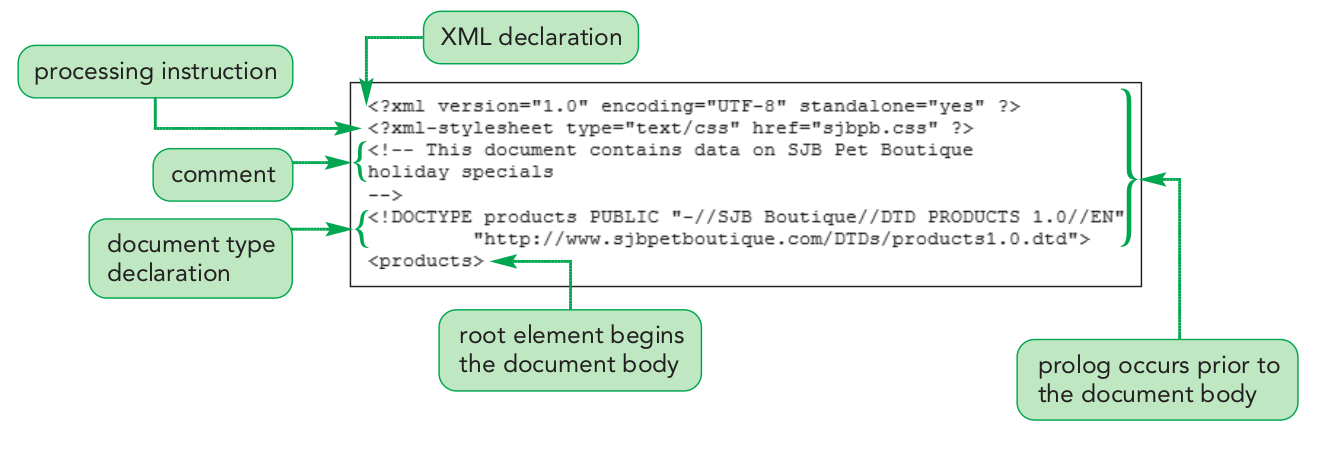
\includegraphics[width=0.95\textwidth]{imgs/XML-Prologo.png}
    \end{center}
\begin{tiny}\textit{immagine dal libro New Perspectives on XML, 3rd Edition}\end{tiny}

\end{frame}

% \begin{frame}
% 	\frametitle{Fondamenti XML}
% 	\framesubtitle{eXtensible Markup Language}
% 	\addtocounter{nframe}{1}

% 	\begin{block}{Esercizio prologo}
% 		Creare un file \textit{.xml} ed inserire un prologo con la dichiarazione XML e un commento con le vostre informazioni.
% 	\end{block}

% 	\begin{block}{Esercizio prologo}
% 		\texttt{
% 		 <!--
% 		 	This document contains data on Codifica di Testi.
% 		 	\\Filename: project.xml
% 		 	\\Author: your name
% 		 	\\Date: today's date
% 		-->
% 		}
% 	\end{block}

% 	\begin{tiny}
% 		\textit{Salvare il file su github nel repository del progetto}
% 	\end{tiny}

% \end{frame}

\begin{frame}
	\frametitle{Fondamenti XML}
	\framesubtitle{eXtensible Markup Language}
	\addtocounter{nframe}{1}

	\begin{block}{XML parser}
		Un programma che legge ed interpreta un documento XML è chiamato XML parser ( o processor).
	\end{block}
	\begin{block}{Cosa fa un XML parser}
		\begin{itemize}
			\item Verifica che il documento rispetti la sintassi XML
			\item Interpreta i dati con tipo PCDATA (\textit{Parsed})
			\item Risolve character or entity references
			\item Gestisce le processing instructions per interpretare i dati
		\end{itemize}
	\end{block}

\end{frame}

% \begin{frame}
% 	\frametitle{Fondamenti XML}
% 	\framesubtitle{eXtensible Markup Language}
% 	\addtocounter{nframe}{1}

% 	\begin{block}{XMLlint}
% 		\begin{center}
% 			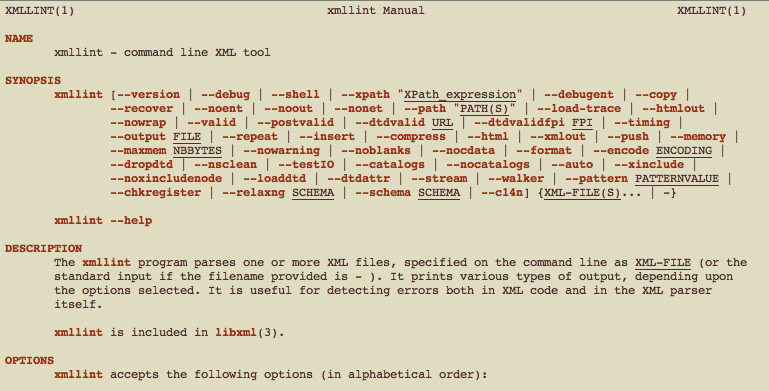
\includegraphics[width=0.95\textwidth]{imgs/xml-XMLlint-man.png}
% 		\end{center}
% 	\end{block}

% \end{frame}


\begin{frame}
    \frametitle{Fondamenti XML}
    \framesubtitle{eXtensible Markup Language}
    \addtocounter{nframe}{1}

	\begin{block}{XML body}
		Un documento XML è composto da elementi e attributi. 
	   \\ Gli elementi sono la base, le unità fondamentali di qualsiasi documento XML.
    \end{block}

    \begin{block}{Elementi: Sintassi}
    \begin{center}\texttt{<element>content</element>}\end{center}
    \begin{center}\texttt{opening tag: <element>;\\ closing tag: </element>}\end{center}
	\end{block}
	\begin{tiny}
		\textit{Un elemento può contenere testo e/o ulteriori elementi}
	\end{tiny}
	
\end{frame}

\begin{frame}
    \frametitle{Fondamenti XML}
    \framesubtitle{eXtensible Markup Language}
    \addtocounter{nframe}{1}

	\begin{block}{XML Element}
		\textit{Gli elementi XML possono avere diversi tipi di contenuto}:
		\begin{itemize}
			\item contenuto strutturale: solo altri elementi, non testo
			\item contenuto misto: testo e anche altri elementi
			\item contenuto testuale: solo testo, non altri elementi
		\end{itemize}
	\end{block}
	
\end{frame}

\begin{frame}
    \frametitle{Fondamenti XML}
    \framesubtitle{eXtensible Markup Language}
    \addtocounter{nframe}{1}

	\begin{block}{XML Element: note importanti sul nome}
		\begin{itemize}
			\item Gli elementi sono case sensitive.
			\item Gli elementi possono iniziare con una lettera o con un ``\_''.
			\item Un elemento non può iniziare con la stringa \textit{xml}. 
			\item Il tag di apertura e di chiusura devono avere lo stesso nome.
			\item Un tag può essere usato più di una volta.
			\item Un insieme di elementi costituiscono un vocabolario
		\end{itemize}
	\end{block}
\end{frame}




% There are a few important points to remember about XML elements:
% • Element names are case sensitive, which means that, for example, itemnumber,
% itemNumber, and ItemNumber are unique elements.
% • Element names must begin with a letter or the underscore character ( \_ ) and may not
% contain blank spaces. Thus, you cannot name an element Item Number , but you can
% name it Item\_Number .
% • Element names cannot begin with the string xml because that group of ­characters is
% reserved for special XML commands.
% • The name in an element’s closing tag must exactly match the name in the ­opening tag.
% • Element names can be used more than once, so the element names can mean
% different things at different points in the hierarchy of an XML document.

% Element names might be established already if an author is using a particular XML
% vocabulary, such as TEI-XML

% Creating XML Elements
% XML 24
% • To create an XML element, use the syntax
% <element>content</element>
% where element is the name given to the element, content represents the text
% content of the element, <element> is the opening tag, and <
% ­ /element> is the
% closing tag.
% • To create an empty XML element with a single tag, use the following syntax:
% <element />
% • To create an empty XML element with a pair of tags, use the syntax
% <element></element>

\begin{frame}
    \frametitle{Fondamenti XML}
    \framesubtitle{eXtensible Markup Language}
    \addtocounter{nframe}{1}

	\begin{block}{XML Element: empty e nested}
		\begin{itemize}
			\item Un elemento vuoto (\textit{empty}) è un elemento senza contenuto.
			\item Un elemento può contenere altri elementi opportunamente annidati (\textit{nested element}).
		\end{itemize}
	\end{block}

	\begin{block}{XML esempi: empty e nested element}
		\begin{itemize}
			\item \texttt{<element />} \texttt{<element></element>}
			\item \texttt{<choice><sic>testo con errore</sic><cor> testo corretto</cor></choice>}
		\end{itemize}
		
	\end{block}
	
\end{frame}


% ESEMPIO
% <product>
% <productName>Dog Shirt Gift Basket</productName>
% <manufacturer>SJB Pet Boutique</manufacturer>
% <description>Something for every day of the week</description>
% <price>35.99</price>
% <price>26.79</price>
% <productItems>1200, 1201, 1202, 1203, 1204, 1205, 1206
% </productItems>
% </product>

\begin{frame}
    \frametitle{Fondamenti XML}
    \framesubtitle{eXtensible Markup Language}
    \addtocounter{nframe}{1}

	\begin{block}{XML Element: hierarchical relationship}
		\begin{itemize}
			\item Un elemento annidato (\textit{nested}) è un elemento \textit{figlio}, cioè contenuto (annidato) in un ulteriore elemento detto padre/genitore (\textit{parent}).
			\item Gli elementi che sono presenti su uno stesso livello gerarchico (\textit{side by side}) sono detti \textit{sibling element}.
		\end{itemize}
	\end{block}

\end{frame}

\begin{frame}
	\frametitle{Fondamenti XML}
	\framesubtitle{eXtensible Markup Language}
	\addtocounter{nframe}{1}

	\begin{center}
		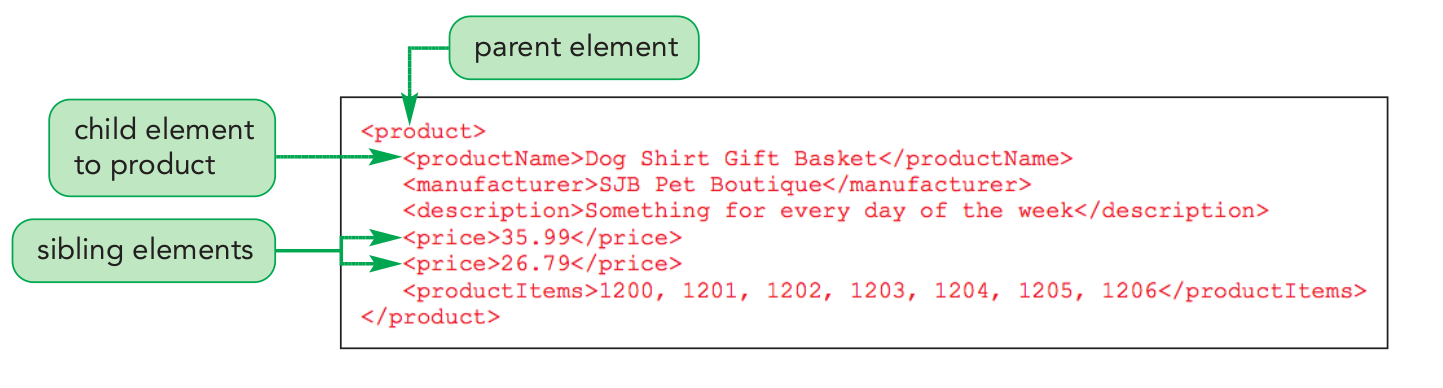
\includegraphics[width=0.95\textwidth]{imgs/XML-Parent-Child-Sibling.png}
    \end{center}
\begin{tiny}\textit{immagine dal libro New Perspectives on XML, 3rd Edition}\end{tiny}

\end{frame}

\begin{frame}
    \frametitle{Fondamenti XML}
    \framesubtitle{eXtensible Markup Language}
    \addtocounter{nframe}{1}

	\begin{block}{XML Element: hierarchical relationship}
		\begin{itemize}
			\item Tutti gli elementi nel body del documento sono figli di uno stesso elemento, chiamato radice (\textit{root}).
			\item Un documento XML deve contenere un elemento root per essere considerato ben formato.
			\item Una gerarchia XML può essere rappresentata tramite un diagramma ad albero.
		\end{itemize}
	\end{block}

\end{frame}

\begin{frame}
    \frametitle{Fondamenti XML}
    \framesubtitle{eXtensible Markup Language}
    \addtocounter{nframe}{1}

	\begin{block}{XML Element: hierarchical relationship cont.}
		\begin{itemize}
			\item Il prologo e i commenti non fanno parte dell'albero del body.
			\item Elementi non annidati correttamente implicano un errore di sintassi nei parser.
			\item Le specifiche XML non consentono di sovrapporre i tag di apertura e di chiusura degli elementi annidati (\textit{no overlap}).
		\end{itemize}
	\end{block}

\end{frame}


% \begin{frame}
%     \frametitle{Fondamenti XML}
%     \framesubtitle{eXtensible Markup Language}
%     \addtocounter{nframe}{1}

% 	\begin{block}{XML Element: hierarchical relationship - Esercizio}
% 		\begin{center}
% 			Scrivere e fare il check di un xml non opportunamente annidato
% 		\end{center}
% 	\end{block}

% \end{frame}

% However, by indenting the code and placing siblings on their own lines, you can visually
% reveal the hierarchy relationships and add a dimension of visual communication to your
% code.

% \begin{frame}
%     \frametitle{Fondamenti XML}
%     \framesubtitle{eXtensible Markup Language}
%     \addtocounter{nframe}{1}

% 	\begin{block}{XML Element: hierarchical relationship as tree structure}
% 		Un modo rapido e comodo per visualizzare la struttura completa di un documento XML è quello di disegnare attraverso un diagramma ad albero ordinato gli elementi del documento XML.
% 	\end{block}

% \end{frame}

% It would be useful to have a general tree diagram that indicates whether a particular
% child element can occur zero times, once, or several times within a parent

% The symbols ?, *, and + are part of the code used in creating DTDs to validate XML
% documents.

% \begin{frame}
% 	\frametitle{Fondamenti XML}
% 	\framesubtitle{eXtensible Markup Language}
% 	\addtocounter{nframe}{1}

% 	\begin{center}
% 		%aggiornare immagine

% 		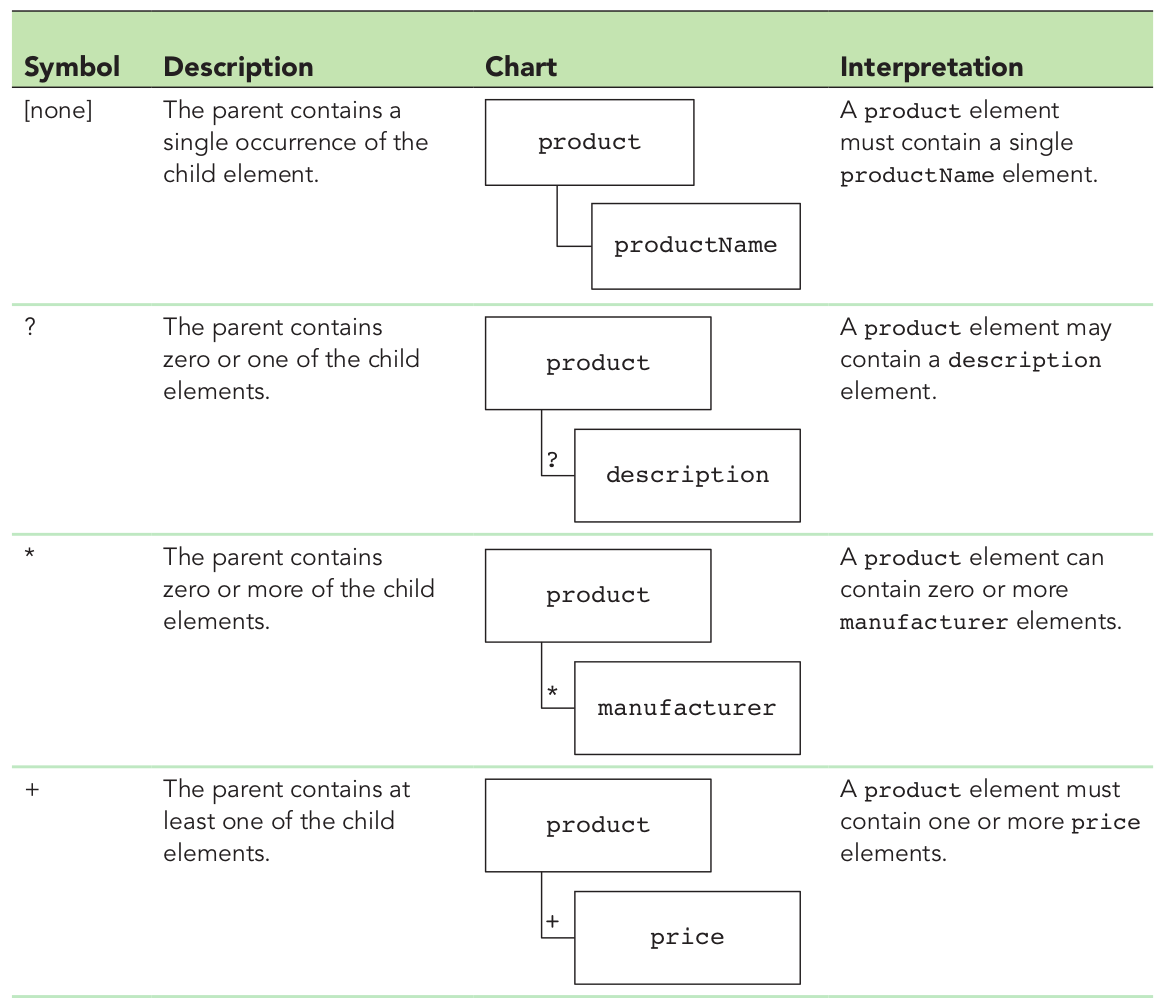
\includegraphics[width=0.8\textwidth]{imgs/xml-parent-child-quantifier.png}
%     \end{center}
    
% \begin{tiny}\textit{immagine dal libro New Perspectives on XML, 3rd Edition}\end{tiny}

% \end{frame}

\begin{frame}
	\frametitle{Fondamenti XML}
	\framesubtitle{eXtensible Markup Language}
	\addtocounter{nframe}{1}

	\begin{center}
		
		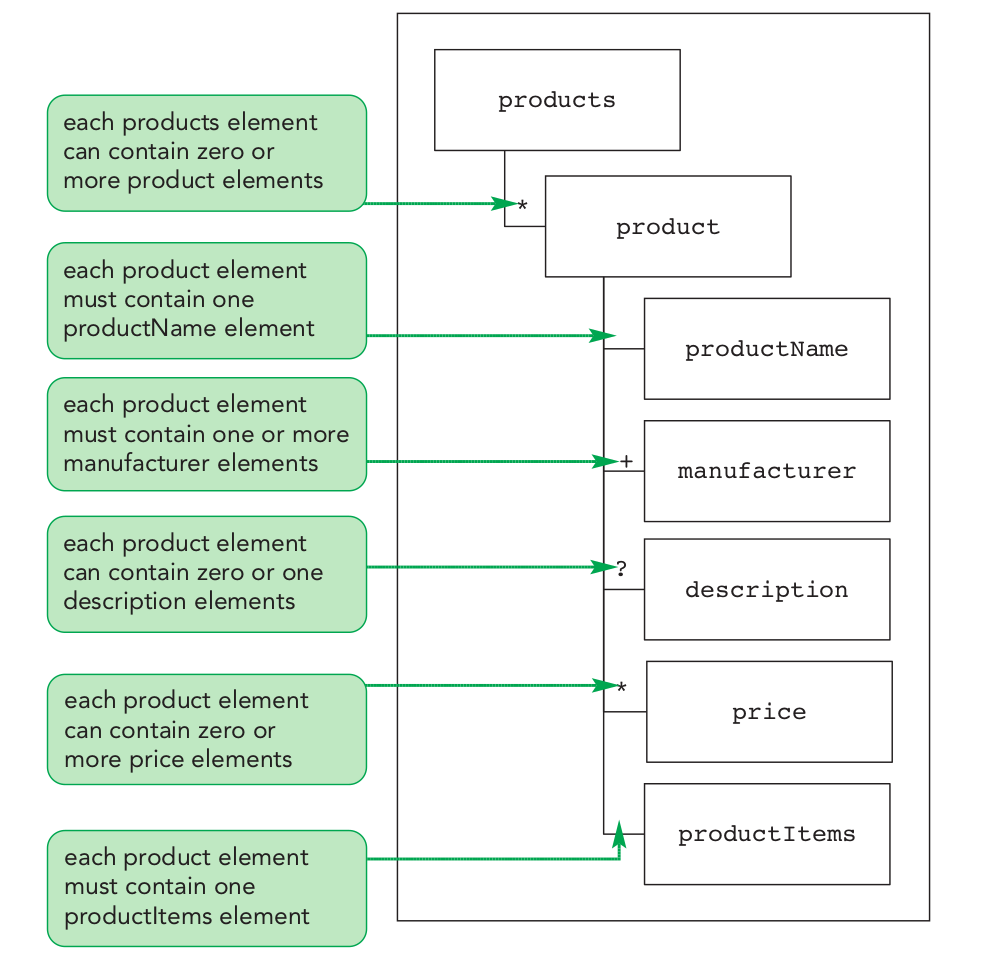
\includegraphics[width=0.7\textwidth]{imgs/xml-parent-child-quantifier2.png}
	\end{center}
\begin{tiny}\textit{immagine dal libro New Perspectives on XML, 3rd Edition}\end{tiny}
\end{frame}


\begin{frame}
    \frametitle{Fondamenti XML}
    \framesubtitle{eXtensible Markup Language}
    \addtocounter{nframe}{1}

	\begin{block}{XML Element: Mixed Content}
		Un elemento può contenere contemporaneamente sia testo sia altri elementi. 
		\\Questo modello di contenuto si chiama Mixed Content ed è ideale per descrivere informazioni text-based (\textbf{dati semi-strutturati)}.
	\end{block}

	\begin{block}{XML Element: Mixed Content}
		\texttt{
			<p><salutation>Salve</salutation> il mio nome è <persName>Angelo</persName></p>
			} 
	\end{block}


\end{frame}

% \begin{frame}
%     \frametitle{Fondamenti XML}
%     \framesubtitle{eXtensible Markup Language}
%     \addtocounter{nframe}{1}

% 	\begin{block}{XML Element: Esercizio}
% 		Aprire il file XML non ben formato presente nel repository github:
% 		\begin{itemize}
% 			\item validarlo con XMLlint
% 			\item correggerlo (commentando gli errori e le modifiche)
% 			\item aggiungere un figlio (child) ad un elemento
% 			\item aggiungere un fratello (sibling) ad un elemento
% 		\end{itemize}
% 	\end{block}

% \end{frame}


\begin{frame}
    \frametitle{Fondamenti XML}
    \framesubtitle{eXtensible Markup Language}
    \addtocounter{nframe}{1}

	\begin{block}{XML Attributi}
		Gli elementi in un documento XML possono avere uno o più attributi.
		\\ Un attributo descrive una caratteristica dell'elemento in cui appare.
	\end{block}

	\begin{block}{XML Attributi}
		Un attributo ha senso solo all'interno del proprio elemento e non è possibile separarlo da esso in alcun modo.
	\end{block}

\end{frame}


\begin{frame}
    \frametitle{Fondamenti XML}
    \framesubtitle{eXtensible Markup Language}
    \addtocounter{nframe}{1}

	\begin{block}{XML Attributi: valore}
		Un attributo ha due componenti: nome - valore.
		Il valore di un attributo è una stringa e deve essere sempre racchiusa tra apici (singoli o doppi).
	\end{block}

	\begin{block}{XML Attributi: valore}
		\begin{center}
			\texttt{<element attribute=``value''> ... </element>}
			\\\texttt{<element attribute=``value'' />}
			\\\texttt{<element attribute=``value'', attribute2=``value2'' />}
		\end{center}
	\end{block}

\end{frame}

\begin{frame}
    \frametitle{Fondamenti XML}
    \framesubtitle{eXtensible Markup Language}
    \addtocounter{nframe}{1}

	\begin{block}{XML Attributi: restrizioni ai nomi}
		\begin{itemize}
			\item Il nome di un attributo può iniziare con una lettera oppure underscore.
			\item Gli spazi non sono consentiti in un nome di un attibuto.
			\item Il nome di un attributo non pò iniziare con la stringa \textit{xml}.
		\end{itemize}
	\end{block}

	\begin{block}{XML Attributi}
		\begin{itemize}
			\item Il nome degli attributi è \textit{case sensitive}.
			\item L'ordine degli attributi non è significativo.
		\end{itemize}
	\end{block}

\end{frame}


% Esercizio con gli attributi:
% (preso dalla TEI)


% Adding an Attribute to an Element
% • To add an attribute to an element, use the syntax
% <element attribute=”value”> ... </element>
% where element is the name given to the element, attribute is the ­attribute’s
% name, and value is the attribute’s value.
% • To add an attribute to a single-sided tag, use the syntax
% <element attribute=”value” />
% • To specify multiple attributes for a single element, use the syntax
% <element attribute1=”value1” attribute2=”value2” ...> ... </element>
% where attribute1 is the first attribute’s name, value1 is the first attribute’s value,
% attribute2 is the second attribute’s name, value2 is the second ­attribute’s
% value, and so on. Each attribute is separated by a space.



% It’s not always clear when to use an attribute value rather than inserting a new element.
% A general rule of thumb is that if all of the XML tags and their attributes were
% removed from a document, the remaining text should comprise the document’s content
% or information.
% Another rule of thumb is that attributes should be used to describe data, but should
% not contain data themselves.
% Different developers have different preferences, and
% there’s no right answer.

% \begin{frame}
%     \frametitle{Fondamenti XML}
%     \framesubtitle{eXtensible Markup Language}
%     \addtocounter{nframe}{1}

% 	\begin{block}{XML Character and Entity References}
% 		\begin{itemize}
% 			\item numeric character reference: \&\#nnn;
% 			\item character entity reference: \&entity;
% 		\end{itemize}
% 	\end{block}

% 	\begin{block}{XML References}
% 		\begin{itemize}
% 			\item \texttt{\&\#65;} (\textit{carattere A})
% 			\item \texttt{\&amp;} (\textit{carattere \&})
% 		\end{itemize}
% 	\end{block}

% \end{frame}

% Inserting Character and Entity References
% • To insert a character reference into an XML document, use
% \&\#nnn;
% where nnn is a character reference number from the ISO/IEC character set.
% • To insert an entity reference, use
% \&entity;
% where entity is a recognized entity name.

% Immagine
% \begin{frame}
% 	\frametitle{Fondamenti XML}
% 	\framesubtitle{eXtensible Markup Language}
% 	\addtocounter{nframe}{1}

% 	\begin{center}
% 			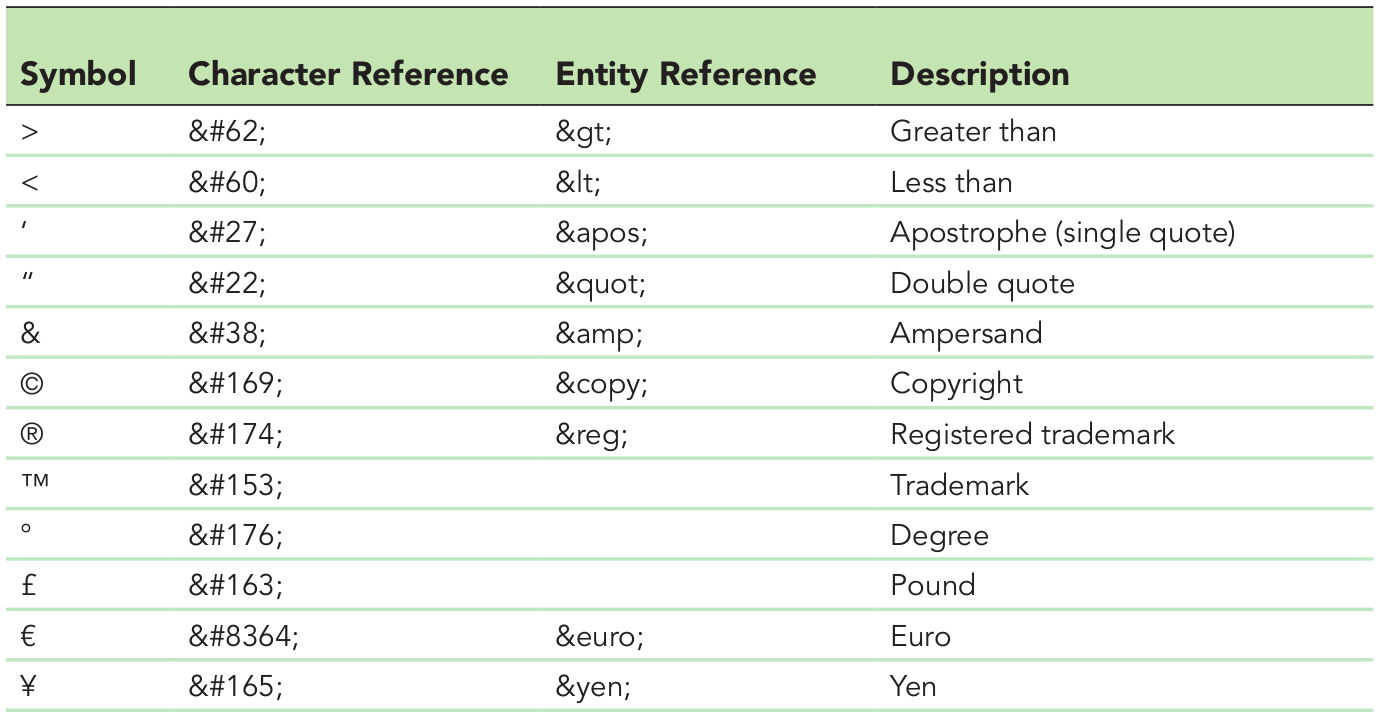
\includegraphics[width=0.95\textwidth]{imgs/xml-Character-Entity.png}
% 	\end{center}
% \begin{tiny}\textit{immagine dal libro New Perspectives on XML, 3rd Edition}\end{tiny}
% \end{frame}


% \begin{frame}
%     \frametitle{Fondamenti XML}
%     \framesubtitle{eXtensible Markup Language}
%     \addtocounter{nframe}{1}

% 	\begin{block}{Text Character Parsing}
% 		Il contenuto testuale di un elemento XML può essere diviso in tre categorie:
% 		parsed character data, character data, and white space.
% 	\end{block}

% 	\begin{block}{Text Character Parsing}
% 		\begin{itemize}
% 			\item \texttt{PCDATA}
% 			\item \texttt{CDATA}
% 			\item \texttt{White Space}
% 		\end{itemize}
% 	\end{block}

% \end{frame}


% \begin{frame}
%     \frametitle{Fondamenti XML}
%     \framesubtitle{eXtensible Markup Language}
%     \addtocounter{nframe}{1}

% 	\begin{block}{Parsed Character Data}
% 		Parsed character data (PCDATA) si riferisce a tutti quei caratteri che XML tratta come parte del codice e quindi vengono interpretati dai parser.
% 	\end{block}

% 	\begin{block}{PCDATA}
% 		\begin{itemize}
% 			\item XML declaration
% 			\item Opening tag e  closing tag
% 			\item Character or entity references
% 			\item Commenti
% 		\end{itemize}
% 	\end{block}

% \end{frame}

% The presence of PCDATA can cause unexpected errors to occur within a document
% This means that symbols such as \&, <, or >, which are all used in ­creating
% markup tags or entity references, are extracted and the appropriate content is used in your program.

% \begin{frame}
%     \frametitle{Fondamenti XML}
%     \framesubtitle{eXtensible Markup Language}
%     \addtocounter{nframe}{1}

% 	\begin{block}{Parsed Character Data}
% 		La presenza di contenuti di tipo PCDATA può causare errori inaspettati.
% 	\end{block}

% 	\begin{block}{XML PCDATA}
% 		Caratteri speciali che sono utilizzati dalla specifica XML come \texttt{\&, <, >} non possono essere utilizzati come contenuto testuale.
% 	\end{block}

% \end{frame}


% Character Data

% \begin{frame}
%     \frametitle{Fondamenti XML}
%     \framesubtitle{eXtensible Markup Language}
%     \addtocounter{nframe}{1}

% 	\begin{block}{Character Data}
% 		I dati di tipo ``Character Data'' non vengono interpretati dal parser XML.
% 		\\ La sequenza di caratteri viene trattata come puro contenuto.
% 		\\In definitiva una sezione \textit{CDATA} è un blocco di testo.
% 	\end{block}

% 	\begin{block}{XML CDATA: sintassi}
% 		\begin{center}
% 			\texttt{
% 				 <![CDATA [
% 					 \\character data
% 					 \\]]>
% 			}
% 		\end{center}
% 	\end{block}

% \end{frame}


%A CDATA section

% \begin{frame}
%     \frametitle{Fondamenti XML}
%     \framesubtitle{eXtensible Markup Language}
%     \addtocounter{nframe}{1}

% 	\begin{block}{Character Data}
% 		Le sezioni di testo CDATA possono essere inserite in qualsiasi parte del documento XML.
% 		\\ Utile per inserire una sezione di testo com molti caratteri speciali.
% 	\end{block}

% \end{frame}

% \begin{frame}
%     \frametitle{Fondamenti XML}
%     \framesubtitle{eXtensible Markup Language}
%     \addtocounter{nframe}{1}

% 	\begin{block}{CDATA: qualche vincolo}
% 		\begin{itemize}
% 			\item Non è possibile inserire commenti in una sezione CDATA.
% 			\item Non è possibile annidare sezioni CDATA. 
% 			\item Non possono essere vuote.
% 			\item i simboli ``]]'' non sono ammessi.
% 		\end{itemize}
% 	\end{block}

% \end{frame}


% \begin{frame}
%     \frametitle{Fondamenti XML}
%     \framesubtitle{eXtensible Markup Language}
%     \addtocounter{nframe}{1}

% 	\begin{block}{Esempio ed esercizio}
% 		Inserire all'interno di un tag un frammento di codice HTML
% 	\end{block}

% 	\begin{block}{CDATA: esempio}
% 		\begin{center}
% 			\texttt{
% 			<htmlCode>
% 			 <![CDATA[
% 			 		<h1>Capitolo Primo</h1>
% 			 		<h2>Sezione Seconda</h2>
% 			 	]]>
% 			 </htmlCode>
% 			 }
% 		\end{center}
% 	\end{block}

% \end{frame}


% White Space

% \begin{frame}
%     \frametitle{Fondamenti XML}
%     \framesubtitle{eXtensible Markup Language}
%     \addtocounter{nframe}{1}

% 	\begin{block}{White Space: esempio}
% 		\begin{itemize}
% 			\item Gli spazi bianchi sono ignorati quando sono tra i tag.
% 			%White space is ignored when it is the only character data between element tags
% 			\item Gli spazi bianchi sono ignorati all'interno del prologo e dell'epilogo e all'interno dei tag. 
% 			%White% space is ignored within a document prolog and epilog, and within any element tags
% 			\item Gli spazi bianchi inseriti nel valore di un attributo sono trattati come parte del contenuto.
% 			%White space within an attribute value is treated as part of the attribute value
% 			\item Non vengono strippati gli spazi all'interno del contentuto testuale degli elementi.
% 			%no white space ­stripping occurs for element content, which means that the content of the XML element
% 		\end{itemize}
% 	\end{block}

% 	\begin{tiny}
% 		I white space sono caratteri non stampabili
% 	\end{tiny}


% \end{frame}

% Inserting a Processing Instruction

% \begin{frame}
%     \frametitle{Fondamenti XML}
%     \framesubtitle{eXtensible Markup Language}
%     \addtocounter{nframe}{1}

% 	\begin{block}{Processing Instruction}
% 		Una \textit{processing instruction} è un comando, una direttiva, che indica al parser XML in che modo elaborare e trattare tutto o parte del documento XML.
% 	\end{block}

% 	\begin{block}{Processing Instruction: sintassi}
% 		\begin{center}
% 			\texttt{<?target instruction ?>}
% 			\\\texttt{<?xml-stylesheet type=”text/css” href=”main.css” media=”all” ?>}
% 		\end{center}
% 	\end{block}
% \begin{tiny}
%     \textit{Molteplici processing instruction possono co-esistere all'interno di un unico documento XML.}
% \end{tiny}
    
% 	% Multiple processing instructions can exist within the same XML document for different
% % media types

% \end{frame}



% \begin{frame}
%     \frametitle{Fondamenti XML}
%     \framesubtitle{eXtensible Markup Language}
%     \addtocounter{nframe}{1}

% 	\begin{block}{Processing Instruction: sintassi}
% 		\begin{center}
% 			\texttt{<?target instruction ?>}
% 			\\\texttt{<?xml-stylesheet type=”text/css” href=”main.css” media=”all” ?>}
% 		\end{center}
% 	\end{block}


% 	\begin{block}{Processing Instruction}
% 		 \textbf{Target}: identifica il tool al quale la processing instruction è diretta.
% 		 \\\textbf{Instruction}: identifica le informazioni che il documento passa al parser per essere elaborate. Le istuzioni hanno la forma degli attributi (nome-valore).
% 	\end{block}

% \end{frame}

% Working with Namespaces

% involves two steps:
% 1. Declare the namespace.
% 2. Identify the elements and attributes within the document that belong to that
% namespace.


% \begin{frame}
%     \frametitle{Fondamenti XML}
%     \framesubtitle{eXtensible Markup Language}
%     \addtocounter{nframe}{1}

% 	\begin{block}{Namespaces}
% 		Un namespace può essere visto come una collezione di elementi e attributi e un insieme di regole che ne determinano la struttura e il contenuto.
% 	\end{block}

% 	\begin{block}{Namespaces}
% 		\begin{center}
% 			\texttt{<element xmlns:prefix=”uri”> ... </element>}
% 			\\\texttt{<element xmlns=”uri”> ... </element>}
% 			\\\texttt{<tei:TEI xmlns:tei=``http://www.tei-c.org/ns/1.0''>}
% 			\\\texttt{<TEI xmlns=``http://www.tei-c.org/ns/1.0''>}
% 		\end{center}
% 	\end{block}

% \end{frame}

% (URI)—a text string that uniquely identifies a resource.
% The purpose of a URI is simply to provide a
% unique string of characters that identify a resource.
% One version of a URI is the Uniform Resource Locator (URL)
% URLs serve as a built-in mechanism on the web for generating unique addresses
% Note that although a URI
% doesn’t actually need to point to a real site on the web, it’s often helpful to place
% documentation at the site identified by a URI so users can go there to learn more
% about the XML vocabulary being referenced.


% The number of namespace attributes that can be declared within an element is
% unlimited.

% root element so that each namespace is available to all
% elements within the document

% You can declare a default namespace by omitting the prefix in the namespace ­declaration.
% Any descendant element or attribute is then considered part of this namespace unless a
% different namespace is declared within one of the child elements.


% \begin{frame}
%     \frametitle{Fondamenti XML}
%     \framesubtitle{eXtensible Markup Language}
%     \addtocounter{nframe}{1}

% 	\begin{block}{Namespaces}
% 		Un namespace viene ereditato da tutti gli elementi discendenti dell'elemento in cui esso è stato dichiarato.
% 	\end{block}

% 	\begin{block}{Namespaces}
% 		Generalmente si dichiarano tutti i namespace nell'elemento root così da avere a disposizione tutti gli elementi dei vari namespace in tutto il documento XML
% 	\end{block}

% \end{frame}

% esempio di dichiarazione di vari namespace in un documento XML

% Declaring a Namespace
% • To declare a namespace for an element within an XML document, add the
% xmlns:prefix attribute to the opening tag of the element using the syntax
% <element xmlns:prefix=”uri”> ... </element>
% where element is the element in which the namespace is declared, prefix is the
% namespace prefix, and uri is the URI of the namespace.
% • To declare a default namespace, add the xmlns attribute without specifying a prefix,
% as follows:
% <element xmlns=”uri”> ... </element>

% immagini di riepilogo












% Attributes can only store a value, while elements can also store child elements and attributes.
% An element can appear more than once within a parent node, but an attribute can appear only once. The order of attributes is not significant and there is no way to control the order of attributes in XSD. If the attribute is present the default value is not assigned, even if the value of the attribute is an empty string.
% the default value of elements is assigned only when the element is present and is empty
% Elements are mandatory by default while attributes are optional by default.


%Both HTML and XML use tags in similar ways, often creating distinctly hierarchical structures to present data to users.

% Like HTML documents, XML documents can be created and viewed with a basic text editor such as Notepad or TextEdit. More sophisticated XML editors are available, and using them can make it easier to design and test documents.




% tanti vocabolari XML
% Bioinformatic Sequence Markup
% Language (BSML) Coding of bioinformatic data
% Extensible Hypertext Markup Language
% (XHTML) HTML written as an XML application
% Mathematical Markup Language
% (MathML) Presentation and evaluation of mathematical equations
% and operations
% Music Markup Language (MML) Display and organization of music notation and lyrics
% Weather Observation Definition
% Format (OMF) Distribution of weather observation reports, forecasts, and
% advisories
% Really Simple Syndication (RSS) Distribution of news headlines and syndicated columns
% Synchronized Multimedia Integration
% Language (SMIL) Editing of interactive audiovisual presentations ­involving
% streaming audio, video, text, and any other media type
% Voice Extensible Markup Language
% (VoiceXML) Creation of audio dialogues that feature synthesized
% speech, digitized audio, and speech recognition
% Wireless Markup Language (WML) Coding of information for smaller-screened devices, such
% as PDAs and cell phones

\begin{frame}
    \frametitle{Elementi XML}
    \framesubtitle{Conclusioni}
    \addtocounter{nframe}{1}

    \begin{block}{XML per rappresentare il testo}
    %\begin{center}\texttt{<!DOCTYPE root PUBLIC “id” “uri”>}\end{center}
    %\begin{center}\texttt{standard//owner//description//language}\end{center}
    %\begin{center}\texttt{-//W3C//DTD XHTML 1.0 Strict//EN}\end{center}
        \begin{itemize}
            \item I markup language per supportare la rappresentazione, memorizzazione, pubblicazione di un testo.
            \item XML è un markup language flessibile e potente.
        \end{itemize}

        \begin{itemize}
            \item le istruznioni dei markup language sono per lo più dichiarazioni indicando particolari funzioni del dato.
            \item le istruznioni sono etichette visibili.
        \end{itemize}
        
    \end{block}

\end{frame}

\begin{frame}
    \frametitle{Elementi XML}
    \framesubtitle{Conclusioni}
    \addtocounter{nframe}{1}

    \begin{block}{XML per rappresentare il testo}
    %\begin{center}\texttt{<!DOCTYPE root PUBLIC “id” “uri”>}\end{center}
    %\begin{center}\texttt{standard//owner//description//language}\end{center}
    %\begin{center}\texttt{-//W3C//DTD XHTML 1.0 Strict//EN}\end{center}
        \begin{itemize}
            \item Una sintassi e una grammatica regolano l'applicabilità del linguaggio di marcatura
            \item Sintassi: documento well formed (ben formato)
            \item Grammatica: documento valido
        \end{itemize}

    \end{block}

\end{frame}


\begin{frame}
    \frametitle{Elementi XML}
    \framesubtitle{Conclusioni}
    \addtocounter{nframe}{1}

    \begin{block}{XML per rappresentare il testo}
    %\begin{center}\texttt{<!DOCTYPE root PUBLIC “id” “uri”>}\end{center}
    %\begin{center}\texttt{standard//owner//description//language}\end{center}
    %\begin{center}\texttt{-//W3C//DTD XHTML 1.0 Strict//EN}\end{center}
        \begin{itemize}
            \item XML deriva dal linguaggio SGML.
            \item XML è una specifica del consorzio W3C.
            \item XML è un meta-linguaggio.
            \item XML è plain text.
            \item XML è portabile.
        \end{itemize}

    \end{block}

\end{frame}

\begin{frame}
    \frametitle{Elementi XML}
    \framesubtitle{Conclusioni}
    \addtocounter{nframe}{1}

    \begin{block}{XML per rappresentare il testo}
    %\begin{center}\texttt{<!DOCTYPE root PUBLIC “id” “uri”>}\end{center}
    %\begin{center}\texttt{standard//owner//description//language}\end{center}
    %\begin{center}\texttt{-//W3C//DTD XHTML 1.0 Strict//EN}\end{center}
        \begin{itemize}
            \item XML definisce markup dichiarativi e descrittivi.
            \item XML ha un modello dati ad albero ordinato.
            \item XML può avere associato un tipo di documento (DTD) o uno schema (XSD).
        \end{itemize}

    \end{block}

\end{frame}


\begin{frame}
	\frametitle{Intro Text Encoding Initiative}
	\framesubtitle{Schemi di codifica TEI – Moduli base}
	\addtocounter{nframe}{1}

	\begin{block}{Caratteristiche degli elementi illustrati}
        \begin{itemize}
            \item gli elementi TEI rientrano nelle categorie generali di
            elementi XML che abbiamo visto
            \item elementi che possono contenere solo altri elementi (=
            elementi strutturali)
            \item elementi che possono contenere altri elementi e testo
            \item elementi che possono contenere solo testo
            \item  elementi vuoti (es. \texttt{<pb/>})
            \item  gli elementi vuoti marcano una gerarchia differente
        \end{itemize}
    \end{block}
\end{frame}


% \begin{frame}
% 	\frametitle{Intro Text Encoding Initiative}
% 	\framesubtitle{Gerarchie multiple}
% 	\addtocounter{nframe}{1}

% 	\begin{center}
% 		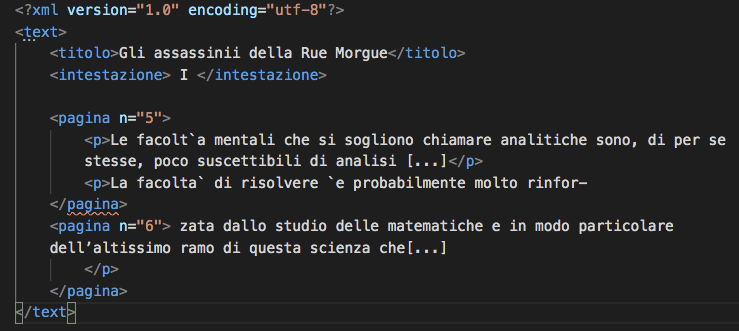
\includegraphics[width=.95\textwidth]{imgs/overlap.png}
% 	\end{center}	
	
%         % \texttt{<?xml version="1.0" encoding="utf-8"?>
%         % <text>
%         % <titolo>Gli assassinii della Rue Morgue</titolo>
%         % <intestazione> I </intestazione>
%         % \emph{<pagina n=``5''>}
%         % <p>Le facoltà mentali che si sogliono chiamare analitiche sono, di
%         % per se stesse, poco suscettibili di analisi [...]</p>
%         % \emph{<p>}La facoltà di risolvere è probabilmente molto rinfor-
%         % \emph{</pagina>}
%         % <pagina n=``6''>
%         % zata dallo studio delle matematiche e in modo particolare
%         % dell’altissimo ramo di questa scienza che[...] \emph{</p>}
%         % </pagina>
% 		% </text>}

% \end{frame}



% \begin{frame}
% 	\frametitle{Intro Text Encoding Initiative}
% 	\framesubtitle{Schemi di codifica TEI – Gerarchie multiple}
% 	\addtocounter{nframe}{1}

% 	\begin{center}
% 		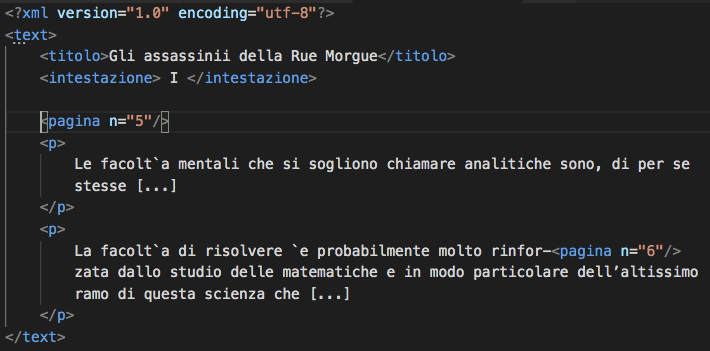
\includegraphics[width=.95\textwidth]{imgs/overlap-b.png}

%         % \texttt{<?xml version="1.0" encoding="utf-8"?>
%         % <text>
%         % <titolo>Gli assassinii della Rue Morgue</titolo>
%         % <intestazione> I </intestazione>
%         % <pagina n="5"/>
%         % <p>Le facoltà mentali che si sogliono chiamare analitiche sono, di
%         % per se stesse [...]</p>
%         % <p>La facoltà di risolvere è probabilmente molto rinfor-
%         % <pagina n="6"/>
%         % zata dallo studio delle matematiche e in modo particolare
%         % dell’altissimo ramo di questa scienza che [...] </p> </text>}
       
%     \end{center}
    
   

% \end{frame}

\begin{frame}
	\frametitle{Intro Text Encoding Initiative}
	\framesubtitle{Schemi di codifica TEI – Moduli base}
	\addtocounter{nframe}{1}

	\begin{block}{Struttura di un documento TEI}
        \begin{itemize}
            \item \textit{struttura fondamentale all’interno della radice (\texttt{<TEI>})}
            \item una intestazione TEI (\texttt{<teiHeader>})
            \item un testo: \texttt{<text>} (o più testi, cfr. infra)
        \end{itemize}
    \end{block}
    
\end{frame}


\begin{frame}
	\frametitle{Intro Text Encoding Initiative}
	\framesubtitle{Schemi di codifica TEI – Moduli base}
	\addtocounter{nframe}{1}

    \begin{block}{Contenuto del TEI header}
        \begin{itemize}
            \item metadati relativi al documento (utili per collezioni di testi
            codificati)
            \item descrizione del file usando \texttt{<fileDesc>} (obbligatoria)
            \item descrizioni relative al tipo di codifica, al contenuto del
            documento, alle sue revisioni (facoltative)
        \end{itemize}
    \end{block}
\textit{E' possibile includere testi introduttivi e spiegazioni relative alla
codifica effettuata (preziosi per l’interscambio!)}

\end{frame}


% \begin{frame}
% 	\frametitle{Intro Text Encoding Initiative}
% 	\framesubtitle{Schemi di codifica TEI:  Moduli base}
% 	\addtocounter{nframe}{1}

% 	\begin{center}

% 		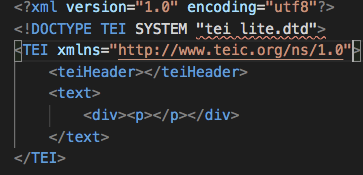
\includegraphics[width=.95\textwidth]{imgs/esempio1.png}
%     %    \texttt{<?xml version="1.0" encoding="utf\-8"?>
%     %      <!DOCTYPE TEI SYSTEM ``tei\_lite.dtd''>
%     %      <TEI xmlns=``http://www.tei\-c.org/ns/1.0''>
%     %      <teiHeader> </teiHeader>
%     %      <text>
%     %          <div>
%     %          <p></p>
%     %          </div>
%     %     </text>
% 	% 	</TEI>}
%     \end{center}
% \end{frame}


\begin{frame}
	\frametitle{Intro Text Encoding Initiative}
	\framesubtitle{Schemi di codifica TEI – Moduli base}
	\addtocounter{nframe}{1}

	\begin{center}
		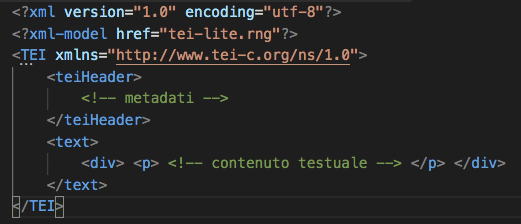
\includegraphics[width=.95\textwidth]{imgs/esempio2.png}
        % \texttt{<?xml version="1.0" encoding="utf-8"?>
        % <?xml-model href="tei-lite.rng"?>
        % <TEI xmlns=``http://www.tei-c.org/ns/1.0''>
        % <teiHeader>...</teiHeader>
        % <text>
        % <div>
        % <p></p>
        % </div>
        % </text>
        % </TEI>}
    \end{center}
    
   

\end{frame}

\begin{frame}
	\frametitle{Intro Text Encoding Initiative}
	\framesubtitle{Schemi di codifica TEI – Moduli base}
	\addtocounter{nframe}{1}

	\begin{block}{documento TEI - schema di intestazione TEI minima}
        Metadati essenziali riguardo il titolo, la modalità di diffusione e
        la fonte originaria di un testo codificato.
        \\Permettono classificazione, archiviazione ed elaborazione
        bibliografica
    \end{block}
    
\end{frame}

% \begin{frame}
% 	\frametitle{Intro Text Encoding Initiative}
% 	\framesubtitle{Schemi di codifica TEI – Intestazione TEI minima}
% 	\addtocounter{nframe}{1}

% 	\begin{center}
% 		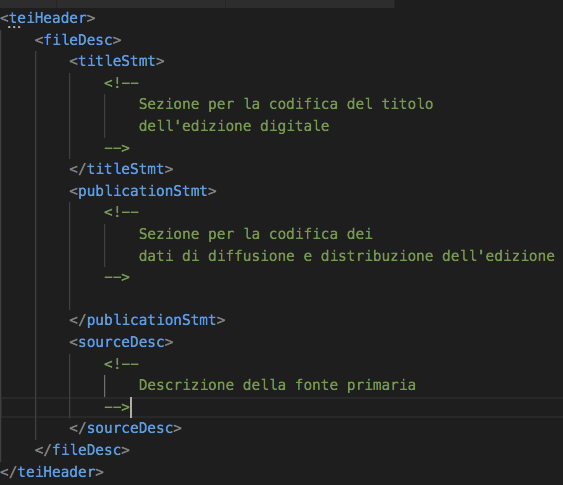
\includegraphics[width=.8\textwidth]{imgs/tei-header.png}
%         % \texttt{<teiHeader>
%         % <fileDesc>
%         % <titleStmt>...</titleStmt>
%         % <publicationStmt>...</publicationStmt>
%         % <sourceDesc>...</sourceDesc>
%         % </fileDesc>
%         % </teiHeader>}
%     \end{center}

% \end{frame}




\begin{frame}
	\frametitle{Intro Text Encoding Initiative}
	\framesubtitle{Schemi di codifica TEI – Moduli base}
	\addtocounter{nframe}{1}

	\begin{center}
		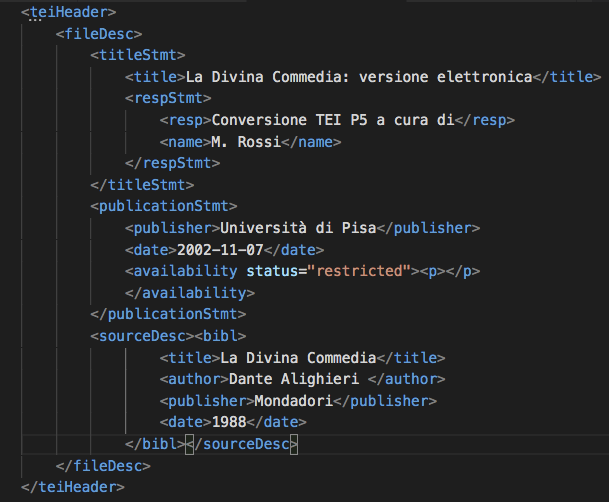
\includegraphics[width=.8\textwidth]{imgs/header2.png}
	\end{center}
	
        % \texttt{<teiHeader>
        % <fileDesc>
        % <titleStmt>
        % <title>La Divina Commedia: versione elettronica</title>
        % <respStmt>
        % <resp>Conversione TEI P5 a cura di</resp><name>M. Rossi</name>
        % </respStmt>
        % </titleStmt>
        % <publicationStmt>
        % <publisher>Università di Pisa</publisher>
        % <date>2002-11-07</date>
        % <availability status=``restricted''><p></p></availability>
        % </publicationStmt>
        % <sourceDesc>
        % <bibl><title>La Divina Commedia</title><author>Dante Alighieri
        % </author><publisher>Mondadori</publisher>
        % <date>1988</date></bibl>
        % </sourceDesc>
        % </fileDesc>
        % </teiHeader>}

\end{frame}



% \begin{frame}
% 	\frametitle{Intro Text Encoding Initiative}
% 	\framesubtitle{Schemi di codifica TEI – Moduli base}
% 	\addtocounter{nframe}{1}

%     \begin{block}{Le altre componenti dell’intestazione TEI}
%         \begin{itemize}
%             \item \texttt{<encodingDesc>} informazioni riguardo lo schema (e il
%             modello di codifica) utilizzato
%             \item  \texttt{<profileDesc>} descrizione del testo: quando è stato
%             creato, da chi, usando quali lingue etc.
%             \item \texttt{<revisionDesc>} informazioni sulle versioni del file
%         \end{itemize}
%     \end{block}
%     \textit{I metadati sono una componente essenziale di qualsiasi
%         progetto di digitalizzazione}
% \end{frame}


% \begin{frame}
% 	\frametitle{Intro Text Encoding Initiative}
% 	\framesubtitle{Schemi di codifica TEI – Moduli base}
% 	\addtocounter{nframe}{1}

% 	\begin{block}{Elementi strutturali}
        
%        \begin{itemize}
%            \item \texttt{<text>} un singolo testo di qualsiasi tipo (punto di partenza della gerarchia).
%            \item \texttt{<facsimile>} riproduzione della fonte primaria, può affiancare o sostituire \texttt{<text>}
%            \item \texttt{<front>} figlio di \texttt{<text>} materiale che precede il testo
%            \item \texttt{<body>} figlio di \texttt{<text>} rappresenta il testo stesso
%            \item \texttt{<back>} figlio di \texttt{<text>} materiale che segue il testo
%            \item \texttt{<group>} figlio di \texttt{<text>} alternativo a \texttt{<body>}, raggruppa testi diversi
%        \end{itemize}
        
%     \end{block}
    
% \end{frame}



\begin{frame}
	\frametitle{Intro Text Encoding Initiative}
	\framesubtitle{Schemi di codifica TEI – Moduli base}
	\addtocounter{nframe}{1}


	\begin{center}
		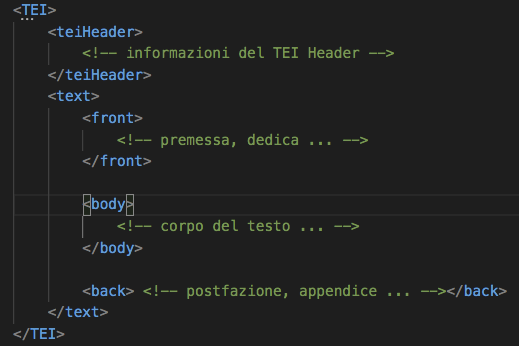
\includegraphics[width=.95\textwidth]{imgs/esempio3.png}
	\end{center}

	% \begin{block}{Esempio schematico di documento TEI}
    %     \texttt{<TEI>
    %     <teiHeader> [informazioni del TEI Header]
    %     </teiHeader>
    %     <text>
    %     <front> [premessa, dedica ...] </front>
    %     <body> [corpo del testo ...] </body>
    %     <back> [postfazione, appendice ...]</back>
    %     </text>
    %     </TEI>}
    % \end{block}
    
   

\end{frame}



% \begin{frame}
% 	\frametitle{Intro Text Encoding Initiative}
% 	\framesubtitle{Schemi di codifica TEI – Moduli base}
% 	\addtocounter{nframe}{1}
%     \begin{block}{Costruire documenti compositi}
%         \begin{itemize}
%             \item rimpiazzando il \texttt{<body>} con un gruppo (\texttt{<group>}) di testi si ottiene un documento composito
%             \item ciascuno di questi testi è rappresentato secondo una struttura
%             standard
%             \item un’altra possibilità è creare un corpus con \texttt{<teiCorpus>}
%             \item intestazioni (\texttt{<teiHeader>}) separate per il corpus e per
%             ciascun gruppo di testi
%             \item struttura più complessa, su più livelli
%         \end{itemize}
%     \end{block}
% \end{frame}


\begin{frame}
	\frametitle{Intro Text Encoding Initiative}
	\framesubtitle{Schemi di codifica TEI – Moduli base}
	\addtocounter{nframe}{1}

	\begin{center}
		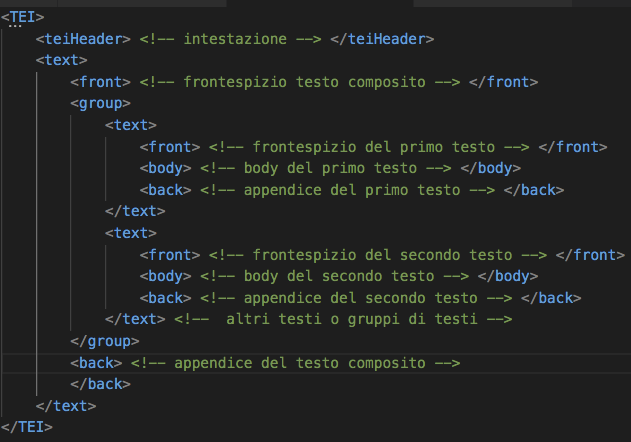
\includegraphics[width=.95\textwidth]{imgs/composito1.png}
	\end{center}

        % \texttt{<TEI>
        % <teiHeader> [ intestazione del testo composito ] </teiHeader>
        % <text>
        % <front> [ front matter del composito ] </front>
        % <group>
        % <text>
        % <front> [ front matter del primo testo ] </front>
        % <body> [ body del primo testo ]
        % </body>
        % <back> [ back matter del primo testo ] </back>
        % </text>
        % <text>
        % <front> [ front matter del secondo testo] </front>
        % <body> [ body del secondo testo ]
        % </body>
        % <back> [ back matter del secondo testo ] </back>
        % </text>
        % ...
        % [ altri testi o gruppi di testi ]
        % ...
        % </group>
        % <back>
        % [ back matter del composito ]
        % </back>
        % </text>
        % </TEI>}

\end{frame}

\begin{frame}
	\frametitle{Intro Text Encoding Initiative}
	\framesubtitle{Schemi di codifica TEI – Moduli base}
	\addtocounter{nframe}{1}
	\begin{center}
		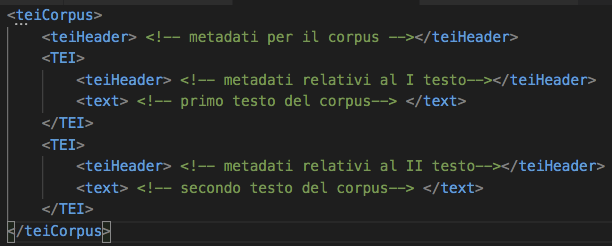
\includegraphics[width=.95\textwidth]{imgs/composito2.png}
	\end{center}

%     \begin{block}{Costruzione di corpora TEI}
%         \texttt{<teiCorpus>
% <teiHeader> [metadati per il corpus] </teiHeader>
% <TEI>
% <teiHeader> [metadati relativi al I testo]</teiHeader>
% <text> [primo testo del corpus] </text>
% </TEI>
% <TEI>
% <teiHeader>[metadati relativi al II testo]</teiHeader>
% <text> [secondo testo del corpus] </text>
% </TEI>
% </teiCorpus>}
%     \end{block}
\end{frame}


% \begin{frame}
% 	\frametitle{Intro Text Encoding Initiative}
% 	\framesubtitle{TEI}
% 	\addtocounter{nframe}{1}

% 	\begin{block}{TEI}
% 	 Schemi di codifica TEI – Moduli base
%   IMMAGINE
%     \end{block}
% \end{frame}


\begin{frame}
	\frametitle{Intro Text Encoding Initiative}
	\framesubtitle{Schemi di codifica TEI – Moduli base}
	\addtocounter{nframe}{1}

	\begin{block}{Altri elementi strutturali fondamentali}
        \begin{itemize}
            \item suddivisioni del testo, non numerati: \texttt{<div> }(nessun limite di nidificazione)
            \item suddivisioni del testo, numerati: \texttt{<div1> ... <div7> }(massimo 7 livelli)
            \item paragrafi: \texttt{<p>}
            \item testo riferito: \texttt{<q>} (discorso diretto, citazioni, etc.)
        \end{itemize}
        
    \end{block}
\end{frame}


\begin{frame}
	\frametitle{Intro Text Encoding Initiative}
	\framesubtitle{Schemi di codifica TEI – Moduli base}
	\addtocounter{nframe}{1}

	\begin{block}{Altri elementi strutturali fondamentali}
        \begin{itemize}
            \item versi: strofe \texttt{<lg>} e singoli versi \texttt{<l>}
            \item testi teatrali: discorsi \texttt{<sp>} che possono contenere paragrafi
            \texttt{<p>} o versi \texttt{<l>}, oltre a direzioni di scena \texttt{<stage>}
            \item milestone tags: \texttt{<pb/>, <lb/>, <cb/>, <milestone/>}
            \item notare che un \texttt{<div>} può contenere un \texttt{<floatingText>} (possibilità di introdurre gerarchie complesse).
        \end{itemize}
        
    \end{block}

\end{frame}

% \begin{frame}
% 	\frametitle{Intro Text Encoding Initiative}
% 	\framesubtitle{Schemi di codifica TEI – Moduli base}
% 	\addtocounter{nframe}{1}

% 	\begin{block}{Apertura e chiusura di un \texttt{<div>}}
%         \begin{itemize}
%             \item \texttt{<head>}: qualunque tipo di intestazione: il titolo di un opera, l’intestazione di un paragrafo, di una sezione, ecc.
%             \item l'attributo \textit{type} permette di classificare in base a una tipologia
%             \item \texttt{<epigraph>} citazione all’inizio del testo, o nella pagina del titolo, eventualmente con riferimento bibliografico
%             \item \texttt{<opener>} raggruppa un serie di elementi (data, luogo, saluti, ecc.) all’inizio del \texttt{<div>}, specie di una lettera
%         \end{itemize}
%     \end{block}

% \end{frame}

% \begin{frame}
% 	\frametitle{Intro Text Encoding Initiative}
% 	\framesubtitle{Schemi di codifica TEI – Moduli base}
% 	\addtocounter{nframe}{1}

% 	\begin{block}{Apertura e chiusura di un \texttt{<div>}}
%         \begin{itemize}
%             \item \texttt{<argument>}: lista degli argomenti trattati nel \texttt{<div>}
%             \item \texttt{<trailer>} frase che compare alla fine del \texttt{<div>} (ad esempio ``Fine del capitolo 1'')
%             \item \texttt{<closer>} raggruppa un serie di elementi (data, luogo, saluti, etc.) alla fine del \texttt{<div>}, specie di una lettera
%         \end{itemize}
%     \end{block}

% \end{frame}


\begin{frame}
	\frametitle{Intro Text Encoding Initiative}
	\framesubtitle{Schemi di codifica TEI – Moduli base}
	\addtocounter{nframe}{1}        
	   
	\begin{center}
		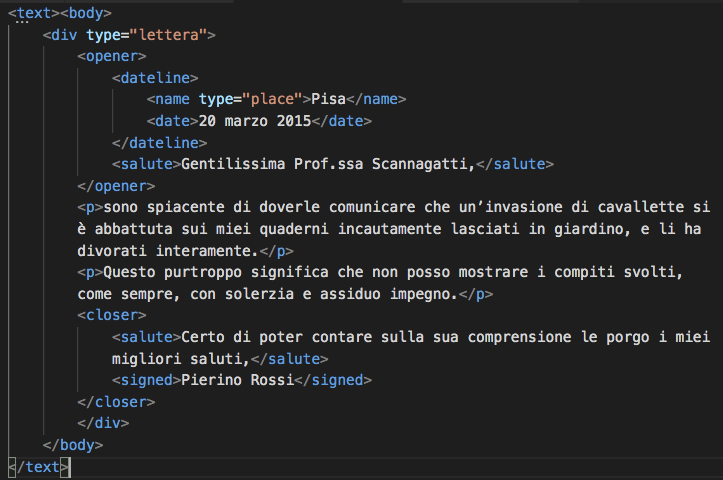
\includegraphics[width=.9\textwidth]{imgs/esLettera.png}
	\end{center}

	% \texttt{<div type="lettera”>
    %     <opener>
    %     <dateline>
    %     <name type=``place''>Pisa</name>
    %     <date>20 marzo 2015</date>
    %     </dateline>
    %     <salute>Gentilissima Prof.ssa Scannagatti,</salute>
    %     </opener>
    %     <p>sono spiacente di doverle comunicare che un’invasione di cavallette si
    %     è abbattuta sui miei quaderni incautamente lasciati in giardino, e li ha
    %     divorati interamente.</p>
    %     <p>Questo purtroppo significa che non posso mostrare i compiti svolti,
    %     come sempre, con solerzia e assiduo impegno.</p>
    %     <closer>
    %     <salute>Certo di poter contare sulla sua comprensione le porgo i miei
    %     migliori saluti,</salute>
    %     <signed>Pierino Rossi</signed>
    %     </closer>
    %     </div>}

\end{frame}





% \begin{frame}
% 	\frametitle{Intro Text Encoding Initiative}
% 	\framesubtitle{Schemi di codifica TEI – Moduli base}
% 	\addtocounter{nframe}{1}

% 	\begin{block}{Errori frequenti}
%         \textit{Si fraintende il significato dell’elemento \texttt{<fileDesc>}}
%         \begin{itemize}
%             \item serve in primo luogo a dare informazioni sul file stesso, non sul testo originale
%             \item il riferimento alla fonte dalla quale è tratto il testo codificato
%             deve essere inserito nel \texttt{<sourceDesc>}
%         \end{itemize}
%     \end{block}

% \end{frame}


% \begin{frame}
% 	\frametitle{Intro Text Encoding Initiative}
% 	\framesubtitle{Schemi di codifica TEI – Moduli base}
% 	\addtocounter{nframe}{1}

% 	\begin{block}{Errori frequenti}
%         I titoli sono codificati con \texttt{<title>} soltanto nel caso di riferimenti bibliografici i titoli del testo, dei capitoli etc. si marcano con \texttt{<head>}
%     \end{block}
    
   

% \end{frame}


% \begin{frame}
% 	\frametitle{Intro Text Encoding Initiative}
% 	\framesubtitle{Schemi di codifica TEI – Moduli base}
% 	\addtocounter{nframe}{1}

% 	\begin{block}{Nota sugli errori possibili}
%         \textbf{Tre categorie:}
%         \begin{itemize}
%             \item \textbf{errori sintattici}: un elemento inserito in un punto sbagliato
%             della gerarchia, o che non può contenere testo etc.
%             \item \textbf{errori di marcatura semantica}: usare un elemento inadatto
%             allo scopo, ad esempio marcare un titolo con <emph>
%             \item \textbf{errori di interpretazione} del testo (che portano al II tipo o
%             all’assenza del markup che andrebbe inserito)
%         \end{itemize}
       
%     \end{block}
%     \textit{Gli errori del primo tipo sono i più facili da individuare e
%         correggere, quelli del terzo i più difficili}

% \end{frame}


% \begin{frame}
% 	\frametitle{Intro Text Encoding Initiative}
% 	\framesubtitle{Schemi di codifica TEI – Moduli base}
% 	\addtocounter{nframe}{1}

% 	\begin{block}{ A proposito di <div>}
%         domanda che ricorre periodicamente: perché non usare nomi
%         più significativi invece di un contenitore generico come <div>
%         (= ‘suddivisione, parte di un testo’)?
%         perché non usare <book>, <chapter>, <section>, etc. come
%         fa, ad esempio, lo schema DOCBOOK?
%         troppa variabilità nell’uso comune, meglio usare un termine
%         generico che possa poi essere specificato usando l’attributo
%         type (es. <div type=”chapter”>)
%         i <div>, numerati o meno, possono essere ‘nidificati’, nessun
%         problema nel riproporre la struttura editoriale visibile
%     \end{block}

% \end{frame}


\begin{frame}
	\frametitle{Intro Text Encoding Initiative}
	\framesubtitle{Schemi di codifica TEI – Moduli base}
	\addtocounter{nframe}{1}

    \textbf{Alcuni attributi possono essere usati con qualsiasi elemento (v. la classe att.global)}

    \begin{block}{ Attributi globali}
        \begin{itemize}
            \item \textbf{n} un numero o un nome non univoco, possibilmente breve, per identificare un elemento
            \item \textbf{rend} informazioni relative all’aspetto (\textit{originale}!) del testo
            \item \textbf{rendition} simile a \textit{@rend}, ma fa riferimento a elementi
            \texttt{<rendition>} inseriti nell’\texttt{<encodingDesc>} (dentro \texttt{<tagsDecl>})
        \end{itemize}
    \end{block}
\end{frame}

\begin{frame}
	\frametitle{Intro Text Encoding Initiative}
	\framesubtitle{Schemi di codifica TEI – Moduli base}
	\addtocounter{nframe}{1}

    \begin{block}{ Attributi globali}
        \begin{itemize}
            \item \textbf{xml:lang} la lingua del testo contenuto da un elemento
            \item \textbf{xml:id} un identificatore univoco per l’elemento
        \end{itemize}
       \textit{NOTA: in base ai moduli usati nello schema sono disponibili ulteriori attributi globali}
    \end{block}
\end{frame}

\begin{frame}
	\frametitle{Intro Text Encoding Initiative}
	\framesubtitle{Schemi di codifica TEI – Moduli base}
	\addtocounter{nframe}{1}

	\begin{center}
		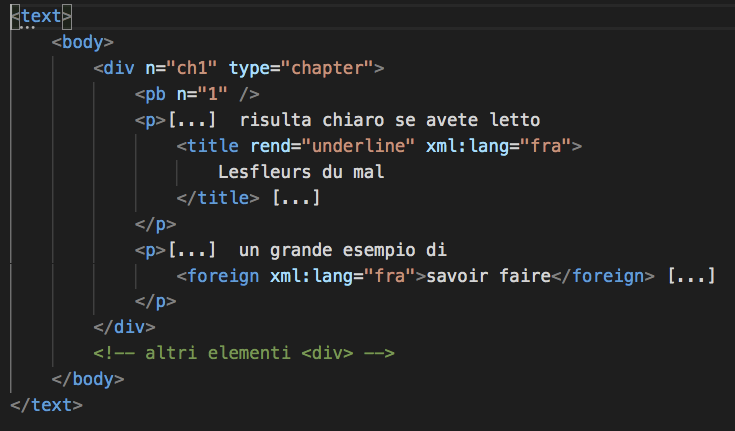
\includegraphics[width=.9\textwidth]{imgs/esempio-attr.png}
	\end{center}
	% \begin{block}{Esempio}
    %     \texttt{<text>
    %     <body>
    %     \emph{<div n="ch1" type=``chapter''>}
    %     <pb n="1"/>[...]
    %     <p>[...] risulta chiaro se avete letto \emph{<title
    %     rend="underline" xml:lang=``fra''>}Les fleurs du
    %     mal</title> [...]</p>
    %     <p>[...] un grande esempio di <foreign
    %     xml:lang=``fra''>savoir faire</foreign> [...]</p>
    %     [...]
    %     </div>
    %     [ altri div ... ]
    %     </body>
    %     </text>}
    % \end{block}

\end{frame}


\begin{frame}
	\frametitle{Intro Text Encoding Initiative}
	\framesubtitle{Schemi di codifica TEI: Moduli base}
	\addtocounter{nframe}{1}

	\begin{center}
		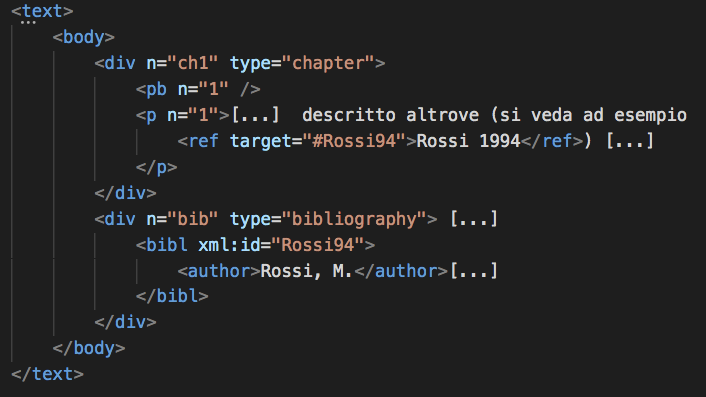
\includegraphics[width=.9\textwidth]{imgs/esempio-attr2.png}
	\end{center}
	% \begin{block}{Esempio}
    %    \texttt{
    %        <text>
    %     <body>
    %     <div n="ch1" type=``chapter''> <pb n="1"/> [...]
    %     <p n=``1''>[...] descritto altrove (si veda ad
    %     esempio \emph{<ref target=``\#Rossi94''>Rossi 1994</ref>})
    %     [...] </p> [...]
    %     </div>
    %     [ altri div ... ]
    %     <div n="bib" type=``bibliography''>
    %     [...]
    %     \emph{<bibl xml:id=``Rossi94''>
    %     <author>Rossi, M.</author>[...]</bibl>}
    %     [...]
    %     </div>
    %     </body>
    %     </text>}
    % \end{block}
\end{frame}

% \begin{frame}
% 	\frametitle{Intro Text Encoding Initiative}
% 	\framesubtitle{Schemi di codifica TEI – Moduli base}
% 	\addtocounter{nframe}{1}

%     \begin{block}{Errori frequenti}
%         \texttt{<div>} non può essere usato allo stesso livello gerarchico
%         di \texttt{<p>}, in altre parole non si può alternare \texttt{<div>} con
%         \texttt{<p>}
%     \end{block}
    
%     \begin{block}{Errore!}
%         \texttt{<div> [...] </div>
%         <p> [...] </p>
%         <div> [...] </div>}
%     \end{block}
% \end{frame}


% \begin{frame}
% 	\frametitle{Intro Text Encoding Initiative}
% 	\framesubtitle{Schemi di codifica TEI – Moduli base}
% 	\addtocounter{nframe}{1}

%     \begin{block}{Errori frequenti}
%         \texttt{<div>} e tutti gli altri elementi strutturali \textit{puri} non
%         possono contenere testo.
       
%     \end{block}
    
%     \begin{block}{Errore!}
%         \texttt{<div>Pippo</div>
%         <person>Pippo</person>}
%     \end{block}
    

% \end{frame}



% \begin{frame}
% 	\frametitle{Intro Text Encoding Initiative}
% 	\framesubtitle{Schemi di codifica TEI – Moduli base}
% 	\addtocounter{nframe}{1}

% 	\begin{block}{Enfasi e termini particolari}
       
%         \begin{itemize}
%             \item \texttt{<emph>} parole o frasi enfatizzate nel testo. (\texttt{Questo è il <emph>mio</emph> computer!})
%             \item \texttt{<foreign>} parola o frase in una lingua diversa. (\texttt{In quel punto entrò il bidello a dare il <foreign xml:lang=``lat''>finis</foreign>}).
%         \end{itemize}
%     \end{block}

% \end{frame}

% \begin{frame}
% 	\frametitle{Intro Text Encoding Initiative}
% 	\framesubtitle{Schemi di codifica TEI – Moduli base}
% 	\addtocounter{nframe}{1}

% 	\begin{block}{Enfasi e termini particolari}
       
%         \begin{itemize}
%             \item \texttt{<distinct>} “diverso” dal testo perché arcaico, gergale, ecc. (\texttt{Saltò in groppa al <distinct>fido destriero</distinct>})
%             \item \texttt{<hi>} elemento generico. (\texttt{<hi rend=``double''>N</hi>el mezzo del cammin di nostra vita.
%             Il suo nome è <hi rend=``italic''>Mario Rossi</hi>})
%         \end{itemize}
%     \end{block}

% \end{frame}

% \begin{frame}
% 	\frametitle{Intro Text Encoding Initiative}
% 	\framesubtitle{Schemi di codifica TEI: Moduli base}
% 	\addtocounter{nframe}{1}

%     \begin{block}{Enfasi e termini particolari}
%         \begin{itemize}
%             \item  \texttt{<mentioned>} parola o frase menzionata ma non usata.
%             (\texttt{Il termine corretto è <mentioned>epigrafe</mentioned>})
%             \item \texttt{<soCalled>} parola o espressione da cui ci si distanzia
%             (\texttt{il cosiddetto <soCalled>darwinismo sociale</soCalled>})
%         \end{itemize}
%     \end{block}
    
% \end{frame}

% \begin{frame}
% 	\frametitle{Intro Text Encoding Initiative}
% 	\framesubtitle{Schemi di codifica TEI: Moduli base}
% 	\addtocounter{nframe}{1}

%     \begin{block}{Enfasi e termini particolari}
%         \begin{itemize}
%             \item \texttt{<term>} una o più parole considerate termine tecnico.
%             (\texttt{Possiamo definire il <term xml\:id="NPL" rend=``italic''>neopositivismo logico</term>})
%             \item \texttt{<gloss>} una spiegazione o glossa riguardo il testo.
%             (\texttt{<gloss target=``\#NPL''>una corrente filosofica basata
%             sul principio che la filosofia debba aspirare al rigore
%             proprio della scienza </gloss>})
%         \end{itemize}
%     \end{block}
    
% \end{frame}

% \begin{frame}
% 	\frametitle{Intro Text Encoding Initiative}
% 	\framesubtitle{Schemi di codifica TEI – Moduli base}
% 	\addtocounter{nframe}{1}

% 	\begin{block}{Esercizio}
%        \textbf{ Marcare un testo plain text di circa 3000 caratteri a piacere.}
%         \begin{itemize}
%             \item inserire prologo XML
%             \item marcare la struttura usando gli elementi fin qui descritti
%             in particolare marcare tutti i paragrafi usando \texttt{<p>} e la struttura editoriale usando \texttt{<div>}
%             \item verificare che sia ben formato con xmllint
%             \item salvare il file XML su github
%         \end{itemize}
%     \end{block}
% \end{frame}

%% sezione relativa alla infrestruttura TEI

% TEI XML focuses on the meaning of text, rather than its appearance.

% TEI XML can be used for a simple reading-oriented transcription of a primary source, whether that be an authorial manuscript, a printed literary work, an audio broadcast, or a dictionary. It can be used for enriched encodings in which many aspects of such texts are made explicit, so that software of all kinds can operate upon them, from visualisation tools and digital publishing systems to specialised statistical analysis packages. It can be used to provide additional annotations and metadata of all kinds.


% deciding on the proper content for that new element does require some knowledge of the way the TEI system is designed




\section{TEI: Codifica Apparato Critico}
% * Evidenziazione, page 1
% Chaucer's Wife of Bath's Prologue

% * Evidenziazione, page 1
% four different manuscripts

% * Evidenziazione, page 1
% El

% * Evidenziazione, page 1
% Hg

% * Evidenziazione, page 1
% La

% * Evidenziazione, page 1
% Ra2

\begin{frame}
    \frametitle{TEI Modulo 12 - Codifica Edizioni Critiche}
    \framesubtitle{Getting started}
    \addtocounter{nframe}{1}
    
    \begin{block}{Main Discipline}
    \end{block}

    \begin{block}{Main Goal}
    \end{block}

\end{frame}

\begin{frame}
    \frametitle{TEI Modulo 12 - Codifica Edizioni Critiche}
    \framesubtitle{Getting started}
    \addtocounter{nframe}{1}

    % * Evidenziazione, page 1
    % Scholarly editions of texts

    % * Evidenziazione, page 1
    % record some or all of the known variations among different witnesses to the text

    % * Evidenziazione, page 1
% variant readings of a text may be accumulated in highly structured form in a critical apparatus of variants.


    \begin{block}{Edizioni critiche di testi}
        Registrare alcune o tutte le varianti presenti nei vari testimoni di un testo
    \end{block}

    \begin{block}{Apparato Critico}
       Nelle edizioni a stampa, i luoghi del testo che presentano letture divergenti sono rappresentate in forma estremamente compressa in specifiche note (\textit{apparati critici}) che accompagnano il testo principale (piè di pagina).
    \end{block}

\end{frame}

\begin{frame}
    \frametitle{TEI Modulo 12 - Codifica Edizioni Critiche}
    \addtocounter{nframe}{1}
    
    \begin{center}
        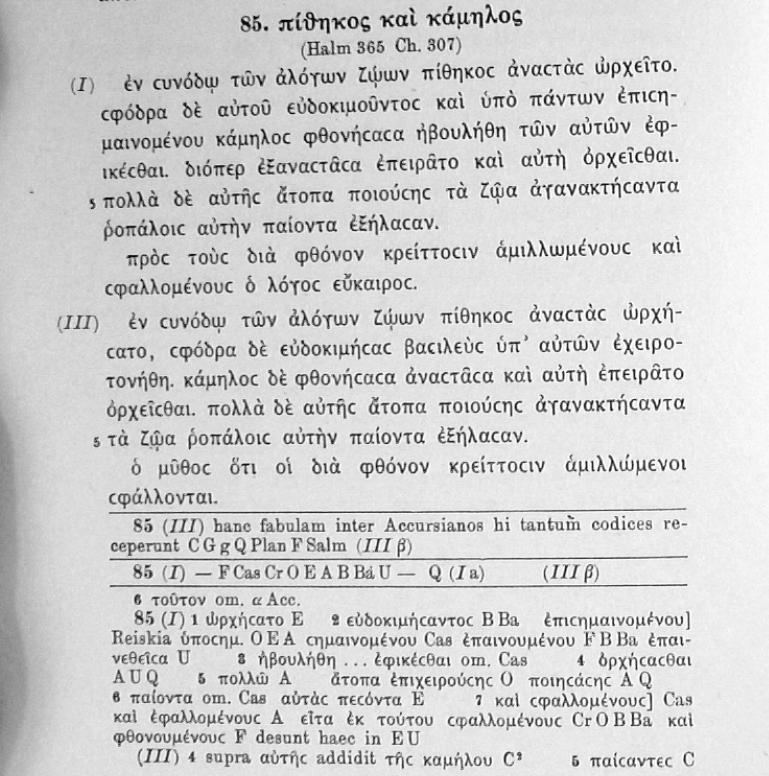
\includegraphics[width=.7\textwidth]{imgs/Edizione-Critica-apparato.png}
    \end{center}

\end{frame}



\begin{frame}
    \frametitle{TEI Modulo 12 - Codifica Edizioni Critiche}
    \framesubtitle{Getting started}
    \addtocounter{nframe}{1}

    
    % * Evidenziazione, page 1
    % Witnesses to a text may include authorial or other manuscripts, printed editions of the work, early translations, or quotations of a work in other texts


    \begin{block}{Edizioni critiche di testi}
        I documenti testimoni di un testo (\textit{tradizione}) possono essere di varia natura:
        \begin{itemize}
            \item manoscritti d'autore
            \item manoscritti copia
            \item edizioni a stampa
            \item traduzioni
            \item citazioni in testimonianze indirette
            \item ...
        \end{itemize}
    \end{block}

\end{frame}

\begin{frame}
    \frametitle{TEI Modulo 12 - Codifica Edizioni Critiche}
    \addtocounter{nframe}{1}
    
    \begin{center}
        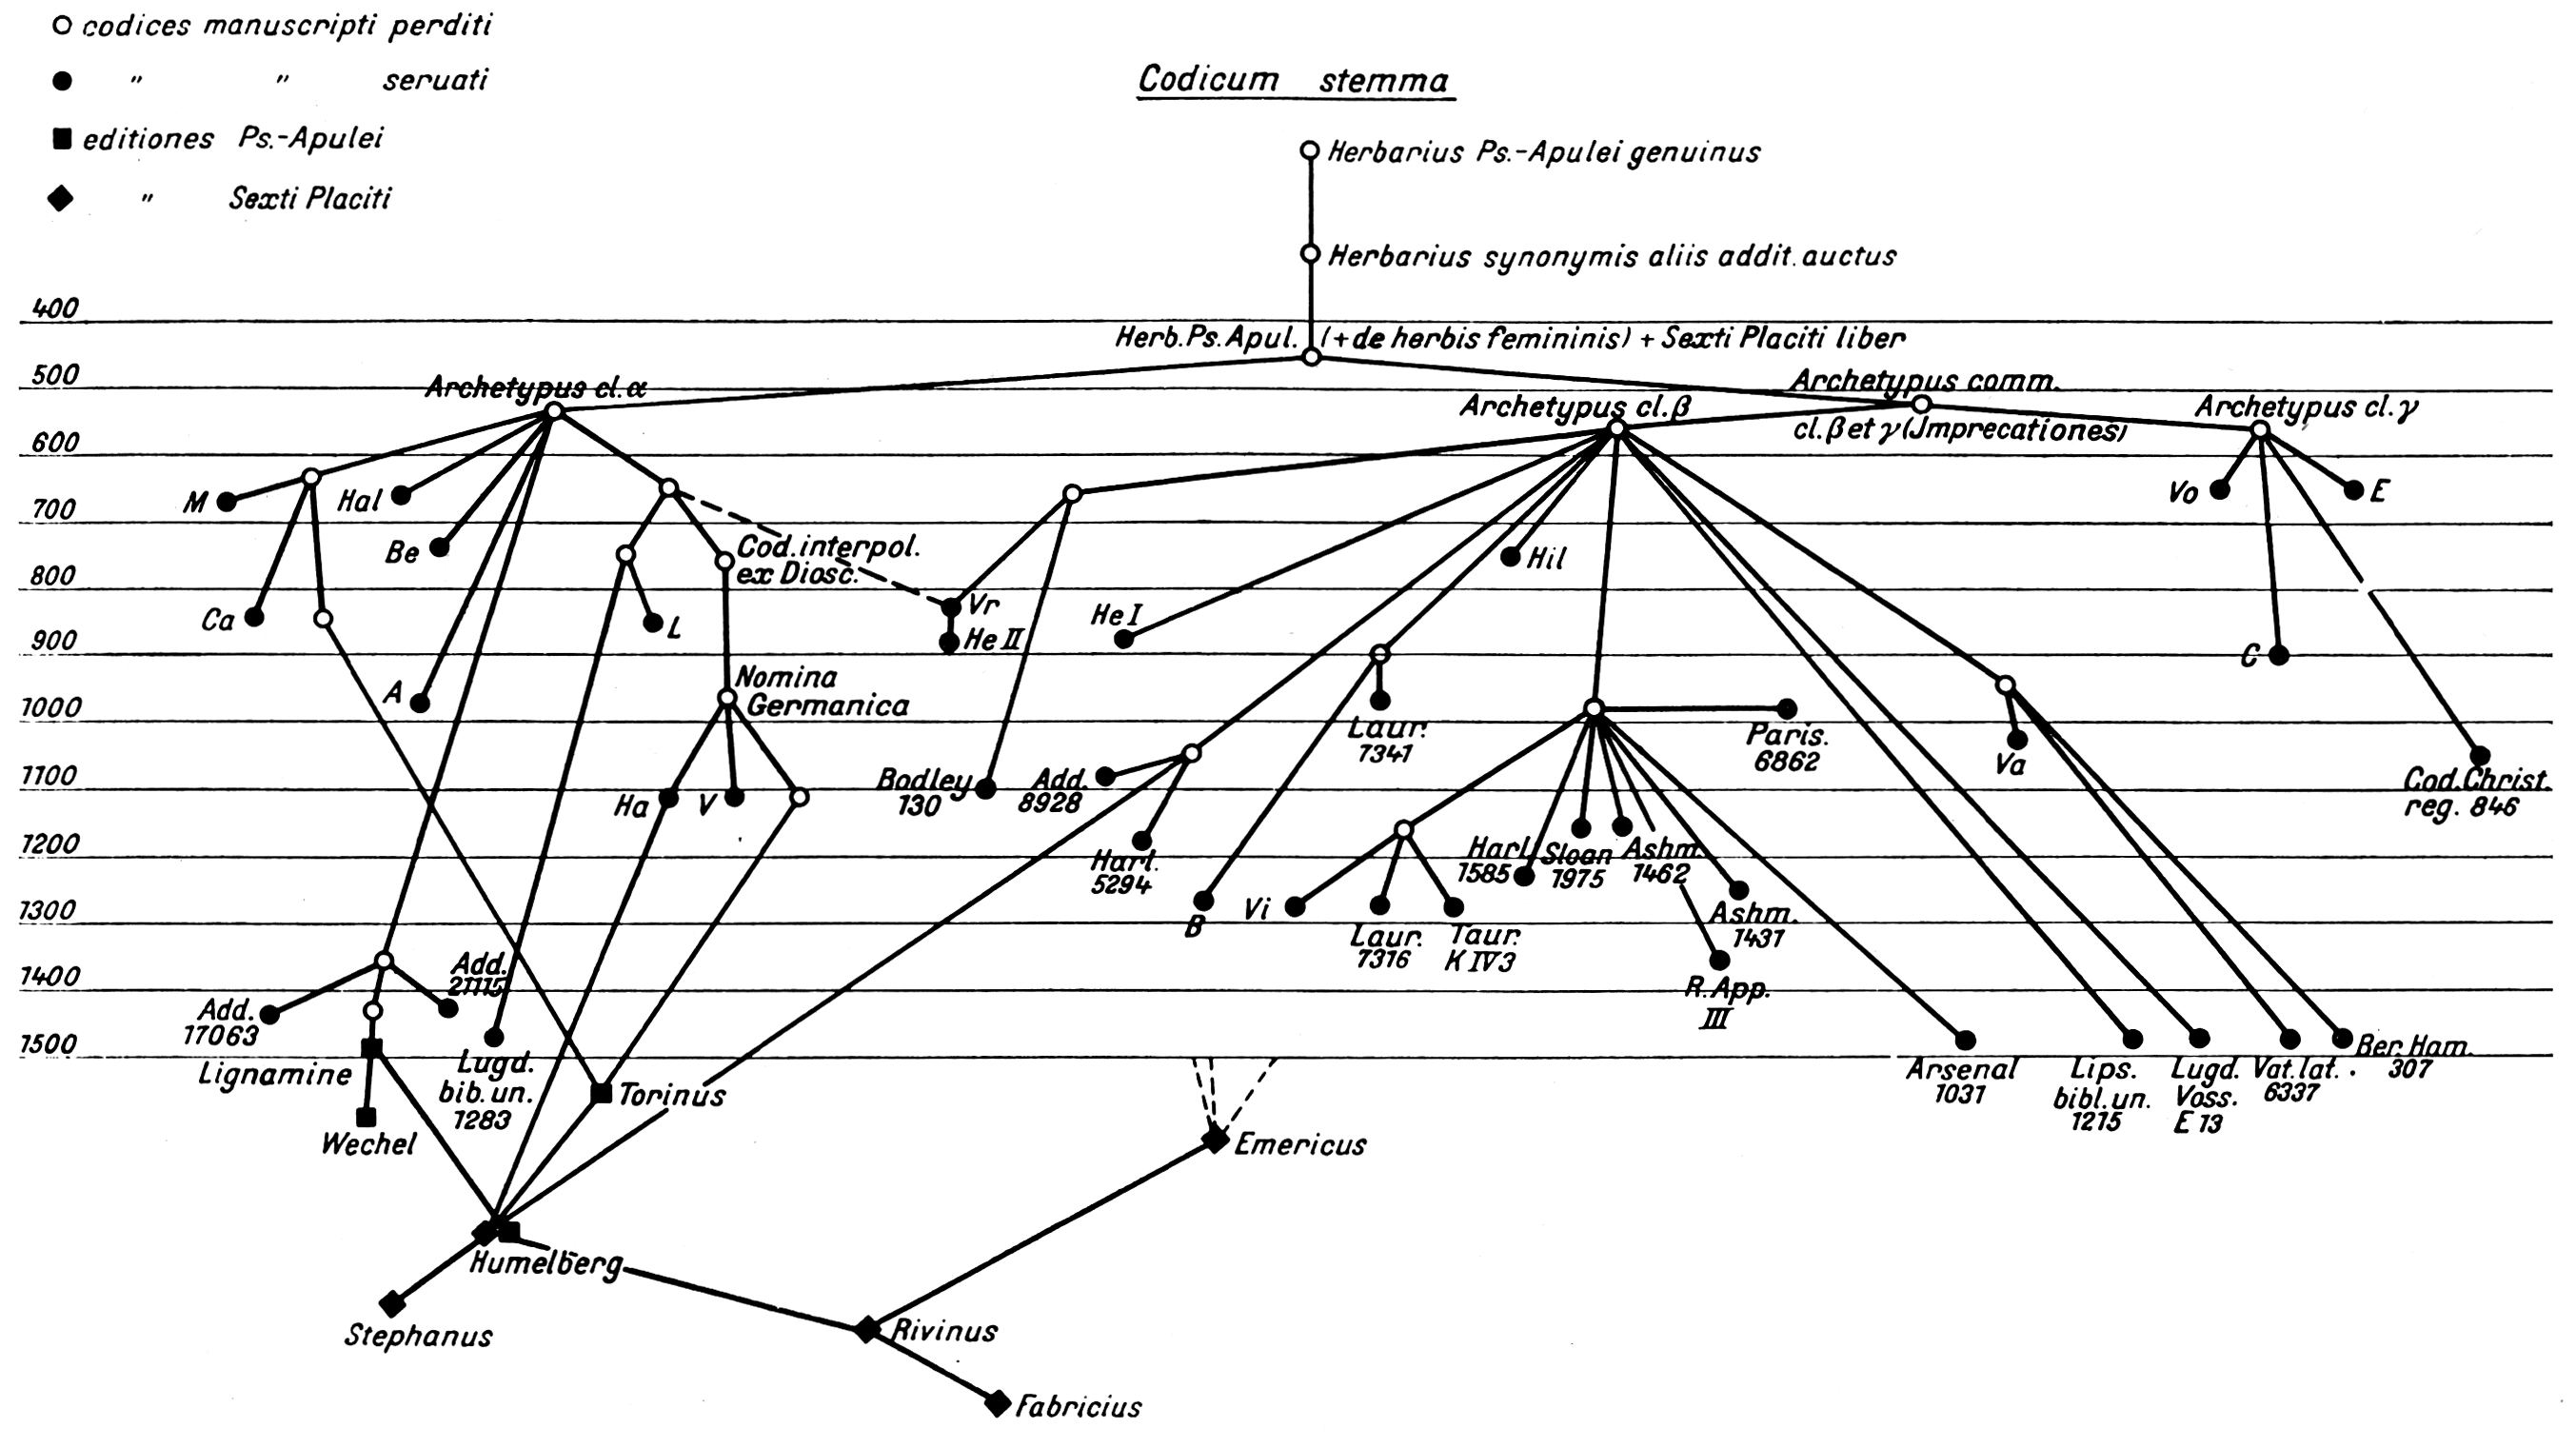
\includegraphics[width=.95\textwidth]{imgs/image.png}
    \end{center}

\end{frame}

\begin{frame}
    \frametitle{TEI Modulo 12 - Codifica Edizioni Critiche}
    \framesubtitle{Getting started}
    \addtocounter{nframe}{1}


    \begin{block}{Cosa rappresenta un apparato critico}
        \begin{itemize}
            \item Rappresentare diverse versioni di uno stesso passo di testo lette da diverse fonti
            \item Accompagnare la scelta dell'editore nel lavoro di ricostruzione del testo
            \item Rappresentare una diramazione del testo nella tradizione e un conseguente ricongiungimento
        \end{itemize}
    \end{block}
       
\end{frame}

\begin{frame}
    \frametitle{TEI Modulo 12 - Codifica Edizioni Critiche}
    \addtocounter{nframe}{1}
    
    \textbf{semplice esempio del grafo delle varianti}

    \begin{center}
        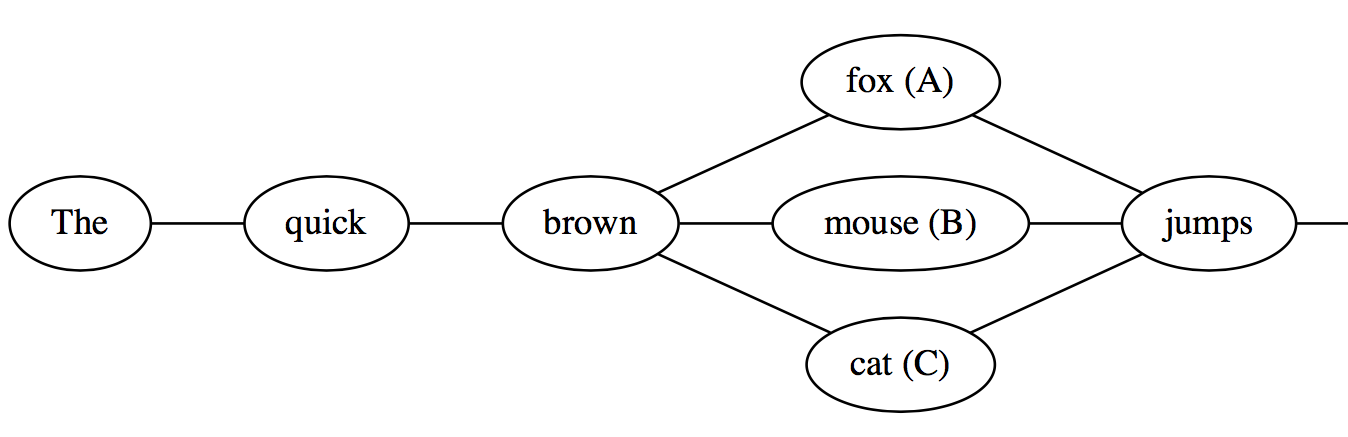
\includegraphics[width=.95\textwidth]{imgs/testo-divergente.png}
    \end{center}

    \textit{image from \url{http://doi.org/10.5281/zenodo.3446155}}

\end{frame}

\begin{frame}
    \frametitle{TEI Modulo 12 - Codifica Edizioni Critiche}
    \framesubtitle{Getting started}
    \addtocounter{nframe}{1}

    % * Evidenziazione, page 1
    % encoding such an apparatus of variants

    % * Evidenziazione, page 1
    % provides extra attributes for some elements of the core tag set when this module is selected
    
    \begin{block}{Obiettivo del modulo 12 (Critical Apparatus)}
        Codificare in forma strutturata l'apparato critico e l'insieme dei testimoni
    \end{block}

    \begin{block}{Modulo 12 delle linee guida TEI}
        Definisce elementi, attributi e prassi per la rappresentazione digitale di edizioni critiche
    \end{block}

\end{frame}

\begin{frame}
    \frametitle{TEI Modulo 12 - Codifica Edizioni Critiche}
    \framesubtitle{Getting started}
    \addtocounter{nframe}{1}

    % * Evidenziazione, page 1
% variant readings

% * Evidenziazione, page 1
% may be recorded in a series of apparatus entries

% * Evidenziazione, page 1
% documentation of the witnesses whose readings are included in the apparatus

    \begin{block}{Modulo 12 delle linee guida TEI}
       Grazie alle specifiche del modulo è possibile registrare la lezione a testo e le lezioni non accolte dei vari testimoni della tradizione
    \end{block}

    \begin{block}{Modulo 12 delle linee guida TEI}
       Documentare i dettagli dei testimoni i quali sono rappresentati con sigle distintive
     \end{block}

\end{frame}

\begin{frame}
    \frametitle{TEI Modulo 12 - Codifica Edizioni Critiche}
    \framesubtitle{Getting started}
    \addtocounter{nframe}{1}


    \begin{block}{Modulo 12 delle linee guida TEI}
        \begin{itemize}
            \item registrare contenuto di testimoni frammentari
            \item registrare le entrate di apparato intercalandole al testo principale (embedded/inline)
            \item registrare le entrate di apparato separate dal testo principale (apparato esterno)
        \end{itemize}
    \end{block}


\end{frame}

\begin{frame}
    \frametitle{TEI Modulo 12 - Codifica Edizioni Critiche}
    \framesubtitle{Apparatus, Readings, Witnesses}
    \addtocounter{nframe}{1}

    % * Evidenziazione, page 1
    % Apparatus

    % * Evidenziazione, page 1
    % Readings

    % * Evidenziazione, page 1
    % Witnesses

    % * Evidenziazione, page 1
    % fundamental markup methods used to encode textual variations

    % * Evidenziazione, page 2
    % the app element for entries in the critical apparatus

    % * Evidenziazione, page 2
    % identifying individual readings

    % * Evidenziazione, page 2
    % ways of grouping readings together

    % * Evidenziazione, page 2
    % identifying which witnesses support a particular reading

    % * Evidenziazione, page 2
    % describing the witnesses included in the apparatus

    % * Evidenziazione, page 2
    % which portions of a text are covered by fragmentary witnesses

    \begin{block}{Elementi fondamentali per la codifica di un testo critico}
        \begin{itemize}
            \item Le singole entrate di apparato sono rappresentate dall'elemento \texttt{<app>}
            \item Le differenti letture sono registrate con l'elemento \texttt{<rdg>}
            \item La lettura accolta a testo è registrata con l'elemento \texttt{<lemma>}
            \item I testimoni sono registrati con l'elemento \texttt{<witness>}
        \end{itemize}
       
    \end{block}


\end{frame}


\begin{frame}
    \frametitle{TEI Modulo 12 - Codifica Edizioni Critiche}
    \framesubtitle{Apparatus, Readings, Witnesses}
    \addtocounter{nframe}{1}

    % * Evidenziazione, page 1
    % Apparatus

    % * Evidenziazione, page 1
    % Readings

    % * Evidenziazione, page 1
    % Witnesses

    % * Evidenziazione, page 1
    % fundamental markup methods used to encode textual variations

    % * Evidenziazione, page 2
    % the app element for entries in the critical apparatus

    % * Evidenziazione, page 2
    % identifying individual readings

    % * Evidenziazione, page 2
    % ways of grouping readings together

    % * Evidenziazione, page 2
    % identifying which witnesses support a particular reading

    % * Evidenziazione, page 2
    % describing the witnesses included in the apparatus

    % * Evidenziazione, page 2
    % which portions of a text are covered by fragmentary witnesses

    \begin{block}{Elementi fondamentali per la codifica di un testo critico}
        \begin{itemize}
            \item Le varianti possono essere raggruppate con l'elemento \texttt{<rgdGrp>}
            \item La tradizione dei testimoni considerati sono raggruppati nell'elemento \texttt{<listWit>}
            \item I testimoni possono essere indicati anche accanto alla variante con l'elemento \texttt{<wit>}
        \end{itemize}
       
    \end{block}

\end{frame}

\begin{frame}
    \frametitle{TEI Modulo 12 - Codifica Edizioni Critiche}
    \framesubtitle{Apparatus, Readings, Witnesses}
    \addtocounter{nframe}{1}

    % * Evidenziazione, page 2
% The app element

% * Evidenziazione, page 2
% The individual apparatus entry is encoded with the app element

% * Evidenziazione, page 2
% a way of marking points where the encoding of a passage in a single source may be carried out in more than one way


% * Evidenziazione, page 2
% Individual textual variations are encoded using the app element

% * Evidenziazione, page 2
% which groups together all the readings constituting the variation

% * Evidenziazione, page 2
% is not a purely mechanical process

% * Evidenziazione, page 2
% Each app element usually comprises one or more readings


    \begin{block}{L'elemento \texttt{<app>}}

        TODO

    \end{block}


\end{frame}


\begin{frame}
    \frametitle{TEI Modulo 12 - Codifica Edizioni Critiche}
    \framesubtitle{Apparatus, Readings, Witnesses}
    \addtocounter{nframe}{1}

    % * Evidenziazione, page 2
% several methods may be used for such linkage

    \begin{block}{Metodi per codificare l'apparato critico}
        \begin{itemize}
            \item location-referenced method
            \item double-end-point-attached method
            \item the parallel segmentation method
        \end{itemize}

       
    \end{block}


\end{frame}


\begin{frame}
    \frametitle{TEI Modulo 12 - Codifica Edizioni Critiche}
    \framesubtitle{Apparatus, Readings, Witnesses}
    \addtocounter{nframe}{1}

    % * Evidenziazione, page 2
    % <app> (apparatus entry) contains one entry in a critical apparatus, with an optional lemma and usually one or more readings or notes on the relevant passage.

    % * Evidenziazione, page 2
    % @type

    % * Evidenziazione, page 2
    % classifies the variation contained in this element according to some convenient typology

    % * Evidenziazione, page 2
    % @from

    % * Evidenziazione, page 2
    % identifies the beginning of the lemma in the base text.

    % * Evidenziazione, page 2
    % @to

    % * Evidenziazione, page 2
    % identifies the endpoint of the lemma in the base text.

    % * Evidenziazione, page 2
    % @loc

    % * Evidenziazione, page 2
    % location

    % * Evidenziazione, page 2
    % indicates the location of the variation

    % * Evidenziazione, page 2
    % The attributes @loc, @from, and @to, are used to link the apparatus entry to the base text

    \begin{block}{L'elemento \texttt{<app>}}
        \texttt{<app>} (\textit{apparatus entry}) contains one entry in a critical apparatus, with an optional lemma and usually one or more readings or notes on the relevant passage.
    \end{block}

\end{frame}

\begin{frame}
    \frametitle{TEI Modulo 12 - Codifica Edizioni Critiche}
    \framesubtitle{Apparatus, Readings, Witnesses}
    \addtocounter{nframe}{1}

    % * Evidenziazione, page 2
    % <app> (apparatus entry) contains one entry in a critical apparatus, with an optional lemma and usually one or more readings or notes on the relevant passage.

    % * Evidenziazione, page 2
    % @type

    % * Evidenziazione, page 2
    % classifies the variation contained in this element according to some convenient typology

    % * Evidenziazione, page 2
    % @from

    % * Evidenziazione, page 2
    % identifies the beginning of the lemma in the base text.

    % * Evidenziazione, page 2
    % @to

    % * Evidenziazione, page 2
    % identifies the endpoint of the lemma in the base text.

    % * Evidenziazione, page 2
    % @loc

    % * Evidenziazione, page 2
    % location

    % * Evidenziazione, page 2
    % indicates the location of the variation

    % * Evidenziazione, page 2
    % The attributes @loc, @from, and @to, are used to link the apparatus entry to the base text

    \begin{block}{Attributi significativi dell'elemento <app>}
        \begin{itemize}
            \item \texttt{@type}: \textit{classifies the variation contained in this element according to some convenient typology}
            \item \texttt{@from}: \textit{identifies the beginning of the lemma in the base text.}
            \item \texttt{@to}: \textit{identifies the endpoint of the lemma in the base text}
            \item \texttt{@loc}: \textit{indicates the location of the variation}
        \end{itemize}
    \end{block}

    \textit{Gli attributi @loc, @from, and @to, sono impiegati per collegare l'entrata di apparato al testo principale (esistono vari metodi)}


\end{frame}

\begin{frame}
    \frametitle{TEI Modulo 12 - Codifica Edizioni Critiche}
    \addtocounter{nframe}{1}
    
    % * Evidenziazione, page 2
    % A very simple partial apparatus

    % * Evidenziazione, page 3
    % in practice the apparatus will be somewhat more complex

    \begin{center}
        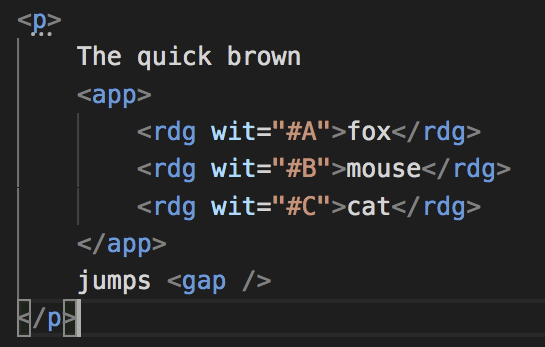
\includegraphics[width=.95\textwidth]{imgs/fox-jumps.png}
    \end{center}

\end{frame}
% * Evidenziazione, page 3
% readings

% * Evidenziazione, page 3
% subvariation

% * Evidenziazione, page 3
% witness information



\begin{frame}
    \frametitle{TEI Modulo 12 - Codifica Edizioni Critiche}
    \framesubtitle{Apparatus, Readings, Witnesses}
    \addtocounter{nframe}{1}

    % * Evidenziazione, page 3
    % Individual readings are the crucial elements in any critical apparatus of variants

    % * Evidenziazione, page 3
    % tag individual readings within an apparatus entry:


    \begin{block}{Registrazione delle diverse lezioni}
        Registrare le singole letture conservate nei singoli testimoni del testo tramandato è l'attività principale per realizzare un apparato delle varianti scientificamente curato 
    \end{block}

    \begin{block}{Registrazione delle diverse lezioni}
        Il vocabolario XML-TEI definisce due elementi per registrare le singole letture 
    \end{block}


\end{frame}


\begin{frame}
    \frametitle{TEI Modulo 12 - Codifica Edizioni Critiche}
    \framesubtitle{Apparatus, Readings, Witnesses}
    \addtocounter{nframe}{1}

% * Evidenziazione, page 3
    % <lem>

    % * Evidenziazione, page 3
    % lemma

    % * Evidenziazione, page 3
    % contains the lemma, or base text, of a textual variation

    % * Evidenziazione, page 3
    % <rdg>

    % * Evidenziazione, page 3
    % reading

    % * Evidenziazione, page 3
    % contains a single reading within a textual variation.

    % * Evidenziazione, page 3
    % the term lemma is used here in the text-critical sense of ‘the reading accepted as that of the original or of the base text’

    \begin{block}{Elementi per la registrazione delle lezioni}
        
        \begin{itemize}
            \item \texttt{<lem>}: \textit{lemma} - contains the lemma, or base text, of a textual variation
            \item \texttt{<rdg>}: \textit{reading} - contains a single reading within a textual variation.
        \end{itemize}

    \end{block}

    \textit{Il termine \textbf{lemma} è inteso nell'accezione di \textbf{lezione accettata dall'editore come lezione a testo, oppure in alternativa come lettura presente nel testo base}}

\end{frame}


\begin{frame}
    \frametitle{TEI Modulo 12 - Codifica Edizioni Critiche}
    \framesubtitle{Apparatus, Readings, Witnesses}
    \addtocounter{nframe}{1}


    % * Evidenziazione, page 3
    % The lem element may also be used to record the base text of the source edition

    % * Evidenziazione, page 3
    % mark the readings of a base witness, to indicate the preference of an editor or encoder for a particular reading, or (e.g. in the case of an external apparatus) to indicate precisely to which portion of the main text the variation applies.

    % * Evidenziazione, page 3
    % may prefer not to use it at all

    \begin{block}{L'elemento texttt{<lem>}}
        
        \begin{itemize}
            \item Usato per registrare il testo di base riportato nella edizione di riferimento
            \item Usato per registrare le lezioni del testimone base di collazione
            \item Usato per registrare la lezione accolta a testo dall'editore dell'edizione critica digitale
            \item Usato per per indicare in modo puntuale a quale porzione del testo principale le letture divergenti si riferiscono
            \item Potrebbe non essere utilizzato affatto
        \end{itemize}

    \end{block}

\end{frame}

\begin{frame}
    \frametitle{TEI Modulo 12 - Codifica Edizioni Critiche}
    \addtocounter{nframe}{1}
    

    \begin{center}
        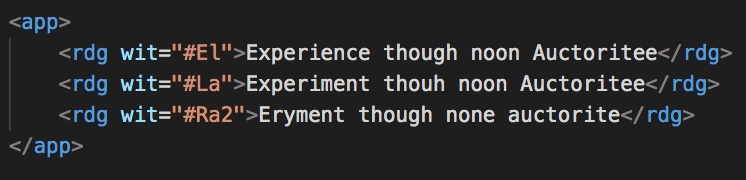
\includegraphics[width=.95\textwidth]{imgs/app-rdg.png}
    \end{center}

\end{frame}


% * Evidenziazione, page 3
% In recording readings within an apparatus entry, the rdg element should always be used; each app usually contains at least one rdg, though it may contain only notes.

% * Evidenziazione, page 3
% How it is used depends in part on the method chosen for linking the apparatus to the text

% * Evidenziazione, page 3
% Readings may be encoded individually, or grouped for perspicuity using the rdgGrp element


\begin{frame}
    \frametitle{TEI Modulo 12 - Codifica Edizioni Critiche}
    \framesubtitle{Apparatus, Readings, Witnesses}
    \addtocounter{nframe}{1}

    \begin{block}{Attributi significativi dell'elemento \texttt{<rdg>} e \texttt{lem}}
        \begin{itemize}
            \item \texttt{@wit}: \textit{(witness or witnesses)} - contains a space-delimited list of one or more pointers indicating the witnesses which attest to a given reading
            \item \texttt{@type}: \textit{} - classifies the reading according to some useful typology. Sample values include: 1] \textit{substantive}; 2] \textit{orthographic}
            \item \texttt{@cause}: \textit{} - classifies the cause for the variant reading, according to any appropriate typology of possible origins. Sample values include: 1] \textit{homeoteleuton}; 2] \textit{homeoarchy}; 3] \textit{paleographicConfusion}; 4] \textit{haplography}; 5] \textit{dittography}; 6] \textit{falseEmendation}
            \item \texttt{@varSeq}: \textit{(variant sequence)} - provides a number indicating the position of this reading in a sequence, when there is reason to presume a sequence to the variants.
        \end{itemize}
    \end{block}

    \textit{le classi di attributi particolarmente utili sono att.witnessed, att.textCritical, att.global.responsibilit, att.global.source, att.written}


\end{frame}

\begin{frame}
    \frametitle{TEI Modulo 12 - Codifica Edizioni Critiche}
    \framesubtitle{Apparatus, Readings, Witnesses}
    \addtocounter{nframe}{1}

      
	
    \begin{block}{Attributi significativi dell'elemento \texttt{<rdg>} e \texttt{lem}}
        \begin{itemize}
            \item \texttt{@hand}: \textit{} - points to a handNote element describing the hand considered responsible for the content of the element concerned
            \item \texttt{@resp}: \textit{(responsible party)} - indicates the agency responsible for the intervention or interpretation, for example an editor or transcriber
            \item \texttt{@cert}: \textit{(certainty)} - signifies the degree of certainty associated with the intervention or interpretation
            \item \texttt{@source}: \textit{} - specifies the source from which some aspect of this element is drawn
            \item \texttt{@exclude}	\textit{} - points to elements that are in exclusive alternation with the current element.
        \end{itemize}
    \end{block}

    \textit{le classi di attributi particolarmente utili sono att.witnessed, att.textCritical, att.global.responsibilit, att.global.source, att.written}


\end{frame}


\begin{frame}
    \frametitle{TEI Modulo 12 - Codifica Edizioni Critiche}
    \framesubtitle{@hand, @source, @resp, @wit}
    \addtocounter{nframe}{1}

    % * Evidenziazione, page 6
    % Encoders should be aware of the distinct fields of use of the attribute values @wit, @hand, and @source

    % * Evidenziazione, page 6
    % @wit identifies the physical entity in which the reading is found (manuscript, clay tablet, papyrus, printed edition);

    % * Evidenziazione, page 6
    % @hand refers to the agent responsible for inscribing that reading in that physical entity (scribe, author, inscriber, hand 1, hand 2)

    % * Evidenziazione, page 6
    % @source indicates the scholar responsible for asserting the existence of that reading in that physical entity

    \begin{block}{Attributi elementi lezioni}
        \texttt{@wit} identifies the physical entity in which the reading is found (manuscript, clay tablet, papyrus, printed edition)
    \end{block}

    \begin{block}{Attributi elementi lezioni}
        \texttt{@hand} refers to the agent responsible for inscribing that reading in that physical entity (scribe, author, inscriber, hand 1, hand 2) 
    \end{block}


\end{frame}


\begin{frame}
    \frametitle{TEI Modulo 12 - Codifica Edizioni Critiche}
    \framesubtitle{@hand, @source, @resp, @wit}
    \addtocounter{nframe}{1}

    % * Evidenziazione, page 6
    % Encoders should be aware of the distinct fields of use of the attribute values @wit, @hand, and @source

    % * Evidenziazione, page 6
    % @wit identifies the physical entity in which the reading is found (manuscript, clay tablet, papyrus, printed edition);

    % * Evidenziazione, page 6
    % @hand refers to the agent responsible for inscribing that reading in that physical entity (scribe, author, inscriber, hand 1, hand 2)

    % * Evidenziazione, page 6
    % @source indicates the scholar responsible for asserting the existence of that reading in that physical entity

    \begin{block}{Attributi elementi lezioni}
        \texttt{@source} indicates the scholars responsible for asserting the existence of that reading in that physical entity
    \end{block}

    \begin{block}{Attributi elementi lezioni}
         \texttt{@resp} indicates the scholars responsible for supplying the intellectual content of the reading reported in the transcription
    \end{block}

\end{frame}

%%%% ESEMPI IMMAGINI %%%%
%%                     %%
\begin{frame}
    \frametitle{TEI Modulo 12 - Codifica Edizioni Critiche}
    \addtocounter{nframe}{1}
    

    \textbf{ESEMPI IMMAGINI!}
    
    \begin{center}
        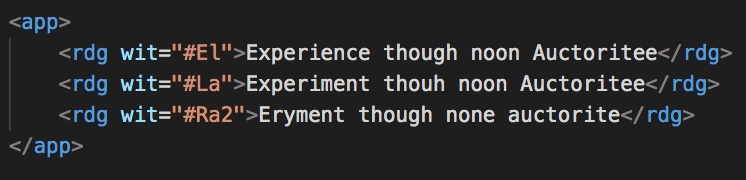
\includegraphics[width=.95\textwidth]{imgs/app-rdg.png}
    \end{center}


\end{frame}

% * Evidenziazione, page 6
% Where there is a greater weight of editorial discussion and interpretation

% * Evidenziazione, page 6
% this information can be attached to the apparatus in a note.

% * Evidenziazione, page 6
% The note element may also be used to record the specific wording of notes in the apparatus of the source edition

% * Evidenziazione, page 6
% <note source="#Kl">

% * Evidenziazione, page 6
% Notes providing details of the reading of one particular witness should be encoded using the specialized witDetail element



% * Evidenziazione, page 6
% the categories may blur: a scholar may produce an edition introducing readings for which he or she is responsible; that edition may itself become a witness in a later critical apparatus.





\begin{frame}
    \frametitle{TEI Modulo 12 - Codifica Edizioni Critiche}
    \framesubtitle{raggruppamento di lezioni e subvariation}
    \addtocounter{nframe}{1}

    % * Evidenziazione, page 6
% Subvariation

% * Evidenziazione, page 6
% The rdgGrp element may be used to group readings

% * Evidenziazione, page 6
% they have identical values on one or more attributes, or because they are seen as forming a self-contained variant sequence, or for some other reason

    \begin{block}{raggrupare diverse lezioni}
        E' possibile raggrupare diverse lezioni con l'elemento \texttt{<rdgGrp>}
    \end{block}

    \begin{itemize}
        \item se più lezioni hanno identici valori per uno o più attributi
        \item se più lezioni son in relazione d'ordine tra lavoro
        \item se più lezioni hanno un qualche tipo di relazione
    \end{itemize}

\end{frame}




\begin{frame}
    \frametitle{TEI Modulo 12 - Codifica Edizioni Critiche}
    \framesubtitle{raggruppamento di lezioni e subvariation}
    \addtocounter{nframe}{1}

    % * Evidenziazione, page 7
    % <rdgGrp>

    % * Evidenziazione, page 7
    % reading group

    % * Evidenziazione, page 7
    % groups two or more readings perceived to have a genetic relationship or other affinity

    % * Evidenziazione, page 7
    % The rdgGrp element is a member of class att.textCritical and therefore can carry the @wit, @type, @cause, @varSeq, @hand, and @resp attributes described in the preceding section.

   

    \begin{block}{raggrupare diverse lezioni}
        \item \texttt{<rdgGrp>} \textit{(reading group)} - within a textual variation, groups two or more readings perceived to have a genetic relationship or other affinity.
    \end{block}

    \begin{center}
       L'elemento \texttt{rdgGrp} può essere caratterizzato dagli stessi attributi dell'elemento \texttt{lem} e dell'elemento \texttt{rdg} \textit{@wit, @type, @cause, @varSeq, @hand, @source, @resp, @exclude}
    \end{center}

\end{frame}


\begin{frame}
    \frametitle{TEI Modulo 12 - Codifica Edizioni Critiche}
    \framesubtitle{raggruppamento di lezioni e subvariation}
    \addtocounter{nframe}{1}

    % * Evidenziazione, page 7
    % When values for any of these attributes are given on a rdgGrp element, the values given are inherited by the rdg or lem elements nested within the reading group
   

    \begin{block}{raggrupare diverse lezioni}
        I valori degli attributi se associati all'elemento \texttt{rdgGrp} vengono ereditati dagli elementi annidati nel gruppo \texttt{rdg} e \texttt{lem}.
    \end{block}


\end{frame}

 

\begin{frame}
    \frametitle{TEI Modulo 12 - Codifica Edizioni Critiche}
    \framesubtitle{raggruppamento di lezioni e subvariation}
    \addtocounter{nframe}{1}
    
    % * Evidenziazione, page 7
    % To indicate that both Hg and La vary only orthographically from the lemma, one might tag both readings <rdg type='orthographic'>

    % * Evidenziazione, page 7
    % This fact can be expressed more perspicuously, however, by grouping their readings into a rdgGrp

    % * Evidenziazione, page 7
    % <app> <lem wit="#El #Ra2">though</lem> <rdgGrp type="orthographic"> <rdg wit="#La">thogh</rdg> <rdg wit="#Hg">thouh</rdg> </rdgGrp> </app>

    \begin{center}
        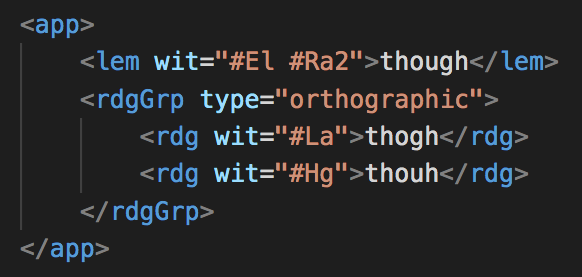
\includegraphics[width=.95\textwidth]{imgs/rdgGrp.png}
    \end{center}


\end{frame}



\begin{frame}
    \frametitle{TEI Modulo 12 - Codifica Edizioni Critiche}
    \framesubtitle{raggruppamento di lezioni e subvariation}
    \addtocounter{nframe}{1}

   % * Evidenziazione, page 7
    % Similarly, rdgGrp may be used to organize the substantive variants of an apparatus entry.

    % * Evidenziazione, page 7
    % Editors may need to indicate that each of a group of witnesses may be taken as all supporting a particular reading

    % * Evidenziazione, page 7
    % manuscripts display many different spellings of these words

    % * Evidenziazione, page 7
    % all these variant spellings and that these variant spellings actually support only the three regularized spelling forms

    % * Evidenziazione, page 7
    % One may term these variant spellings as ‘subvariants’ of the regularized spelling forms.

    % * Evidenziazione, page 7
    % This subvariation can be expressed within an app element by gathering the readings into three groups according to the normalized form of their reading.

    % * Evidenziazione, page 7
    % All the readings within each group may be accounted subvariants of the main reading for the group

    % * Evidenziazione, page 7
    % tagging it as a lem element or as <rdg type='groupBase'>


    \begin{block}{raggrupare diverse lezioni}
        \item \texttt{rgdGrp} può essere utilizzato per raggruppare varianti sostanziali e sottovarianti formali
        \item indicare diverse varianti formali che supportano la stessa variante sostanziale
        \item codificare ciascuna variante sostanziale con l'elemento \texttt{lem} e le varianti formali con l'elemento \texttt{rdg}, tutto all'interno di un elemento \texttt{rdgGrp}
    \end{block}


\end{frame}


\begin{frame}
    \frametitle{TEI Modulo 12 - Codifica Edizioni Critiche}
    \framesubtitle{raggruppamento di lezioni e subvariation}
    \addtocounter{nframe}{1}
    
    % * Evidenziazione, page 7
    % In this example, the different subvariants on Experience, Experiment, and Eriment are held within three rdgGrp elements nested within the enclosing app element:



    % * Evidenziazione, page 8
    % From this, one may deduce that the regularized reading Experience is supported by all three manuscripts El Hg Ha4, although the spelling differs in Ha4, and that the regularized reading Eriment is supported by Ra2, even though the form differs in that manuscript.

    % * Evidenziazione, page 8
    % Thus, Ha4 here supports the reading Experience found in El and Hg, even though it is spelt slightly differently in Ha4.

    % * Evidenziazione, page 8
    % Reading groups may nest recursively, so that variants can be classified to any desired depth.
    

    \begin{center}
        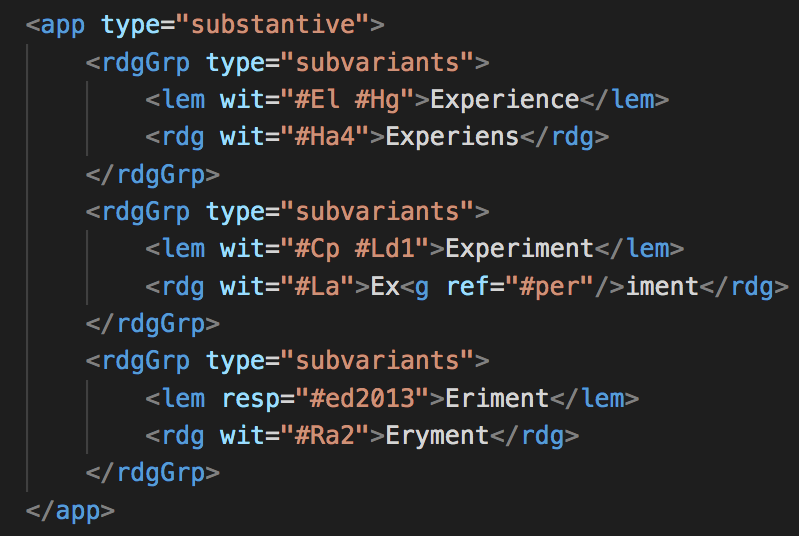
\includegraphics[width=.95\textwidth]{imgs/variant-subvariant.png}
    \end{center}


\end{frame}



\begin{frame}
    \frametitle{TEI Modulo 12 - Codifica Edizioni Critiche}
    \framesubtitle{raggruppamento di lezioni e subvariation}
    \addtocounter{nframe}{1}

  
    % * Evidenziazione, page 8
    % Because apparatus entries may also nest, the app element might also be used to group readings in the same way.

    \begin{block}{raggrupare diverse lezioni}
       Le entrate di apparato, definite con l'elemento \texttt{<app>}  possono essere annidate l'una nell'altra.
    \end{block}
    \begin{block}{raggrupare diverse lezioni}
        Anche l'elemento \texttt{<app>} può essere usato per raggruppare diverse letture seguendo qualche tipo di classificazione.
     \end{block}


\end{frame}



\begin{frame}
    \frametitle{TEI Modulo 12 - Codifica Edizioni Critiche}
    \framesubtitle{raggruppamento di lezioni e subvariation}
    \addtocounter{nframe}{1}
    
    % * Evidenziazione, page 8
    % this variation has three normalized readings, and that the first of these is supported by manuscripts El, Hg, and Ha4; the second by Cp, Ld1, and La; and the third by Ra2

    \begin{center}
        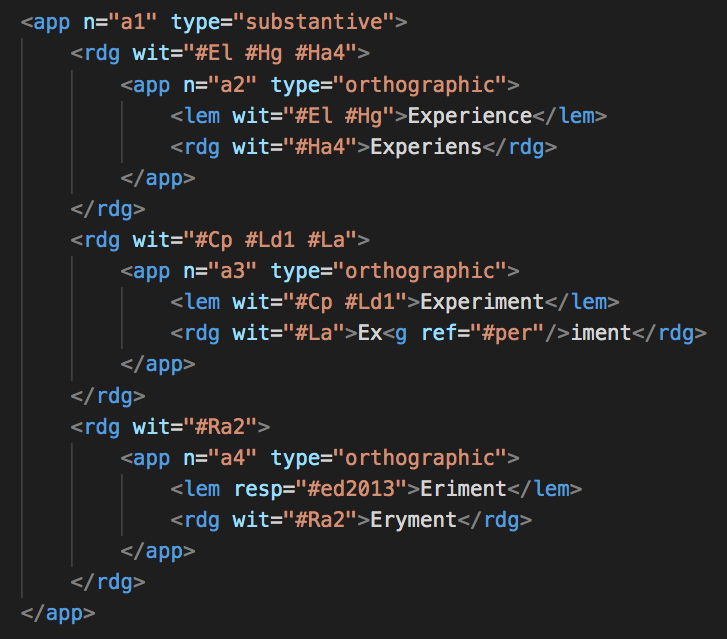
\includegraphics[width=.95\textwidth]{imgs/nest-app.png}
    \end{center}


\end{frame}

\begin{frame}
    \frametitle{TEI Modulo 12 - Codifica Edizioni Critiche}
    \framesubtitle{raggruppamento di lezioni e subvariation}
    \addtocounter{nframe}{1}
    
    % * Evidenziazione, page 8
    % Reading groups may also be used to bring together variants which form an apparent developmental sequence

    \begin{center}
        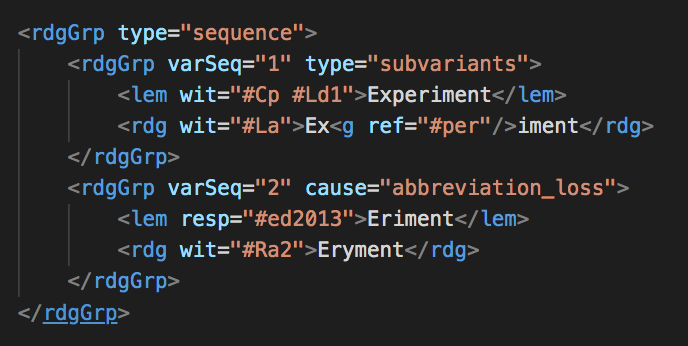
\includegraphics[width=.95\textwidth]{imgs/rdgGrp-seq.png}
    \end{center}


\end{frame}



\begin{frame}
    \frametitle{TEI Modulo 12 - Codifica Edizioni Critiche}
    \framesubtitle{descrizione dei testimoni}
    \addtocounter{nframe}{1}

    \begin{block}{raggrupare diverse lezioni}
      Le informazioni su singoli testimoni può riguardare:
      \begin{itemize}
          \item Associare specifiche informazioni relative ad un testimone tra quelli che concordano sulla stessa lezione
          \item Trascrivere letteralmente le informazioni presenti su un testimone da un edizione di riferimento
          \item Definire l'insieme (più o meno strutturato) dei testimoni recensiti
      \end{itemize}
    \end{block}

\end{frame}



\begin{frame}
    \frametitle{TEI Modulo 12 - Codifica Edizioni Critiche}
    \framesubtitle{descrizione dei testimoni}
    \addtocounter{nframe}{1}

    % * Evidenziazione, page 9
    % A given reading is associated with the set of witnesses attesting it by listing the witnesses in the @wit attribute on the rdg or lem element

    % * Evidenziazione, page 9
    % associate annotation on a reading with one specific witness among several

    % * Evidenziazione, page 9
    % can be linked to both a reading and to one or more of the witnesses for that reading


    \begin{block}{elemento \texttt{<witDetail>}}
     \texttt{<witDetail>} \textit{(witness detail)} - gives further information about a particular witness, or witnesses, to a particular reading
    \end{block}

    \begin{block}{attributi dell'elemento \texttt{<witDetail>}}
        \begin{itemize}
            \item \texttt{@target} \textit{} - specifies the destination of the reference by supplying one or more URI References
            \item \texttt{@wit} \textit{(witnesses)} - indicates the sigil or sigla identifying the witness or witnesses to which the detail refers
        \end{itemize}

    \end{block}

\end{frame}




\begin{frame}
    \frametitle{TEI Modulo 12 - Codifica Edizioni Critiche}
    \framesubtitle{Informazioni sui testimoni}
    \addtocounter{nframe}{1}
    
    % * Evidenziazione, page 8
    % Reading groups may also be used to bring together variants which form an apparent developmental sequence
    % * Evidenziazione, page 9


    % * Evidenziazione, page 9
    % made explicit by the @target attribute

    % * Evidenziazione, page 9
    % the link to the witness, by the @wit attribute

    % * Evidenziazione, page 9
    % @target specifies the destination of the reference

    % * Evidenziazione, page 9
    % @wit (witnesses) indicates the sigil or sigla identifying the witness or witnesses to which the detail refers

    % * Evidenziazione, page 9
    % he witDetail refers to multiple readings, @target must be used to point to the reading(s) being annotated
    
    \begin{center}
        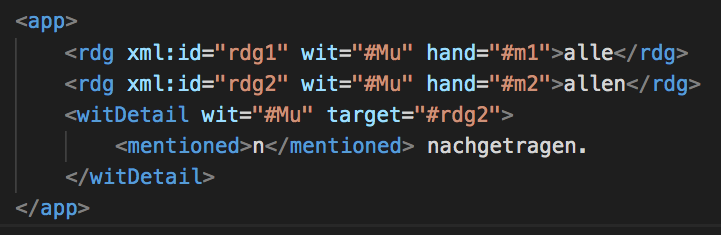
\includegraphics[width=.95\textwidth]{imgs/witDetails.png}
    \end{center}

    % * Evidenziazione, page 10
    % may be used to record the specific wording of information in the source text

    % * Evidenziazione, page 10
    % to record the wording of the note explaining that the variant reading adds n to the original in a second hand

\end{frame}





\begin{frame}
    \frametitle{TEI Modulo 12 - Codifica Edizioni Critiche}
    \framesubtitle{descrizione dei testimoni}
    \addtocounter{nframe}{1}


    \begin{block}{Registrale informazioni sui testimoni}
        \texttt{<wit>} \textit{} - contains a list of one or more sigla of witnesses attesting a given reading, in a textual variation.
    \end{block}

    \begin{center}
        \textit{Usare l'attributo \texttt{@wit} (assieme all'elemento \texttt{<witDetail>} quando necessario) è quasi sempre la scelta più conveniente}
    \end{center}
    
    % * Evidenziazione, page 11
    % @wit is more succinct,

    % * Evidenziazione, page 11
    % using @wit (with witDetail when needed) is almost always to be preferred
\end{frame}

\begin{frame}
    \frametitle{TEI Modulo 12 - Codifica Edizioni Critiche}
    \framesubtitle{Informazioni sui testimoni}
    \addtocounter{nframe}{1}
    
    % * Nota ancorata, page 10
    % nota sigla 

    %The Latin word siglum (sign), pl. sigla denotes the abbreviation used in a critical apparatus to indicate a particular witness

    % * Evidenziazione, page 10
    % lists of sigla

    % * Evidenziazione, page 10
    % may be complex enough

    % * Evidenziazione, page 10
    % in the transcription of printed critical editions, it may be desirable to retain for future reference the exact form in which the source edition records the witnesses to a particular reading;

    % * Evidenziazione, page 10
    % The wit element may be used to transcribe such lists of witnesses to a particular reading.

    % * Evidenziazione, page 10
    % <wit> contains a list of one or more sigla of witnesses attesting a given reading, in a textual variation.

    % * Evidenziazione, page 10
    % The wit list may appear following a rdg, rdgGrp, or lem element in any apparatus entry

    % * Evidenziazione, page 10
    % wit may be used in a way functionally equivalent to @wit if the sigla therein are wrapped in refs with @target attributes pointing to a predefined witness

    
    \begin{center}
        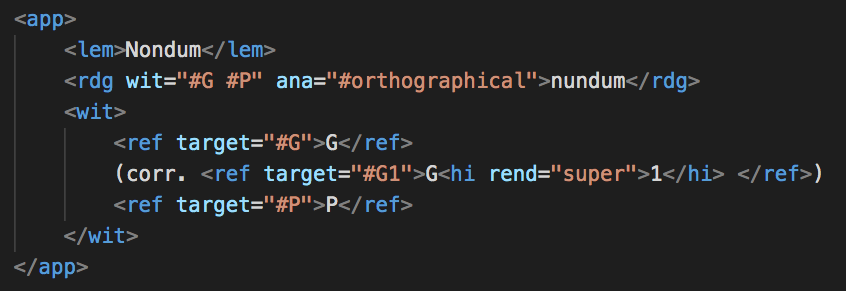
\includegraphics[width=.95\textwidth]{imgs/app-wit.png}
    \end{center}

\end{frame}



\begin{frame}
    \frametitle{TEI Modulo 12 - Codifica Edizioni Critiche}
    \framesubtitle{descrizione dei testimoni}
    \addtocounter{nframe}{1}

    % * Evidenziazione, page 11
    % A list of all identified witnesses should normally be supplied in the front matter of the edition, or in the sourceDesc element of its header

    % * Evidenziazione, page 11
    % may be given either as a simple bibliographic list

    % * Evidenziazione, page 11
    % or as a listWit element,

    % * Evidenziazione, page 11
    % which contains a series of witness elements

    % * Evidenziazione, page 11
    % Each witness element may contain a brief characterization of the witness, given as one or more prose paragraphs
    
    \begin{block}{Insieme dei testimoni recensiti}
        La lista dei testimoni recensita può essere registrata con l'elemento \texttt{<listWit>}
    \end{block}

    \begin{center}{...}
        l'elemento \texttt{<listWit>} contiene a sua volta elementi \texttt{<witness>}. Ciascun elemento \texttt{witness} contiene una breve descrizione del testimone in una forma semi-strutturata. 
    \end{center}
    
   
\end{frame}


\begin{frame}
    \frametitle{TEI Modulo 12 - Codifica Edizioni Critiche}
    \framesubtitle{descrizione dei testimoni}
    \addtocounter{nframe}{1}

    
    \begin{block}{elemento \texttt{<listWit>}}
        \texttt{<listWit>} \textit{(witness list)} - lists definitions for all the witnesses referred to by a critical apparatus, optionally grouped hierarchically.
    \end{block}

    \begin{center}{elemento \texttt{<witness>}}
        \texttt{<witness>} contains either a description of a single witness referred to within the critical apparatus, or a list of witnesses which is to be referred to by a single sigil.
    \end{center}
    
    \textit{La lista dei testimoni è quindi l'insieme delle sigle di tutti i testimoni recensiti e riferiti in apparato}
   
\end{frame}


\begin{frame}
    \frametitle{TEI Modulo 12 - Codifica Edizioni Critiche}
    \framesubtitle{Informazioni sui testimoni}
    \addtocounter{nframe}{1}
    
    
    \begin{center}
        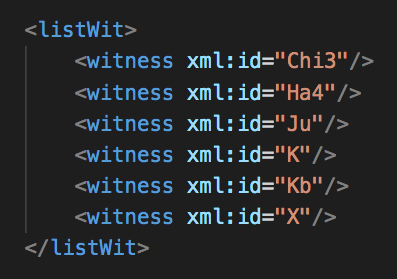
\includegraphics[width=.95\textwidth]{imgs/listWit-base.png}
    \end{center}

\end{frame}


\begin{frame}
    \frametitle{TEI Modulo 12 - Codifica Edizioni Critiche}
    \framesubtitle{Informazioni sui testimoni}
    \addtocounter{nframe}{1}
    
    % * Evidenziazione, page 12
    % each witness element should contain at least a brief prose description of the witness

    % * Evidenziazione, page 12
    % including a bibliographic citation


    % * Evidenziazione, page 12
    % the witness description here may be complemented by a reference to a full description of the manuscript supplied elsewhere, typically as the content of a msDesc or bibl element

    \begin{center}
        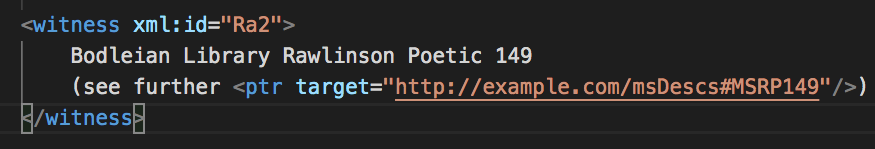
\includegraphics[width=.95\textwidth]{imgs/witness-ref.png}
    \end{center}

    \begin{center}
        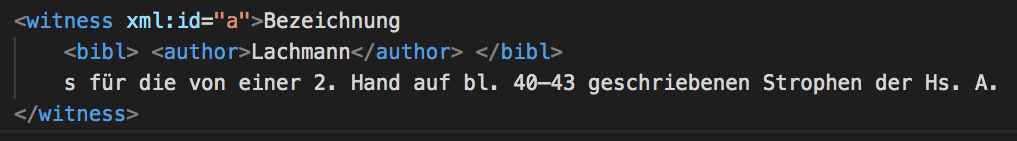
\includegraphics[width=.95\textwidth]{imgs/witness-bibl.png}
    \end{center}

    % * Evidenziazione, page 12
    % a whole paragraph of commentary for each witnes

    % * Evidenziazione, page 13
    % It would however generally be preferable to represent such detailed information using an appropriately structured msDesc element

    % * Evidenziazione, page 13
    % if the witnesses being recorded are not manuscripts but printed works, it may be preferable to document them using the standard bibl or biblStruct elements

\end{frame}




\begin{frame}
    \frametitle{TEI Modulo 12 - Codifica Edizioni Critiche}
    \framesubtitle{descrizione dei testimoni}
    \addtocounter{nframe}{1}

    % * Evidenziazione, page 13
    % In text-critical work it is customary to refer to frequently occurring groups of witnesses by means of a single common siglum

    % * Evidenziazione, page 13
    % including a nested witness list within the witness list

    % * Evidenziazione, page 13
    % uses the siglum for the group as its identifier

    % * Evidenziazione, page 13
    % supplies a fuller name for the group in its optional child head element
    
    \begin{block}{famiglie di testimoni}
        Spesso è utile raggruppare i testimoni in famiglie o in altri tipi di gruppi che riuniscano testimoni con attributi comuni.
    \end{block}
    \begin{block}{famiglie di testimoni}
        Ciò è possibile realizzarlo annidando elementi \texttt{listWit} in altri elementi \texttt{listWit}
    \end{block}
   
\end{frame}


\begin{frame}
    \frametitle{TEI Modulo 12 - Codifica Edizioni Critiche}
    \framesubtitle{Informazioni sui testimoni}
    \addtocounter{nframe}{1}
    
    \begin{center}
        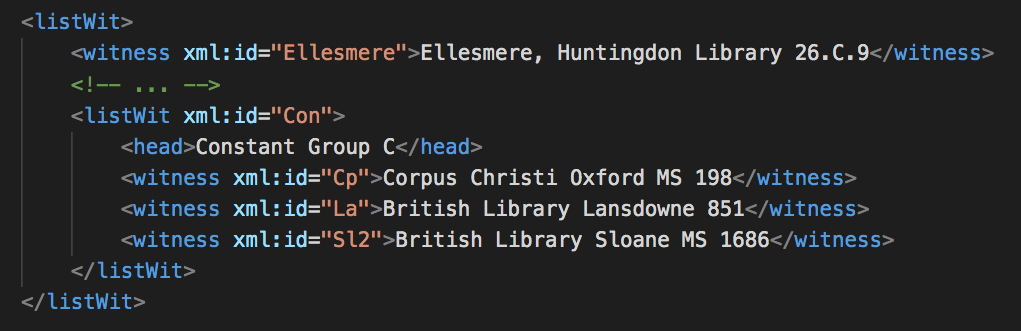
\includegraphics[width=.95\textwidth]{imgs/listWit-nest.png}
    \end{center}


\end{frame}

% * Evidenziazione, page 13
% The more elaborate example below shows both multiple levels of nesting and a strategy for mapping the the @xml:id of the witness to the siglum which will be displayed to the reader of a derived visualisation

% * Evidenziazione, page 13
% <witness xml:id="Σ">Servius (<abbr type="siglum">Σ</abbr>) = ΔΓ

% * Evidenziazione, page 13
% <witness xml:id="Δ">

% * Evidenziazione, page 14
% <abbr type="siglum">Δ</abbr>

% * Evidenziazione, page 14
% <witness xml:id="Γ">

% * Evidenziazione, page 14
% <abbr type="siglum">Γ</abbr>

% * Evidenziazione, page 15
% Here we have a summary of the witnesses, with their sigla, used in an edition, as is generally found in the conspectus siglorum in the front matter of a critical edition.

% * Evidenziazione, page 15
% Families are indicated with Greek letters and manuscript witnesses with Latin letters

% * Evidenziazione, page 15
% The siglum for display is always contained in the abbr with @type ‘siglum’



% * Evidenziazione, page 15
% Situations commonly arise where there are many more or less fragmentary witnesses

% * Evidenziazione, page 15
% there may be quite distinct groups of witnesses for different parts of a text or collection of texts

% * Evidenziazione, page 15
% If a witness list is provided, it may be unnecessary to give, in each apparatus entry, an exhaustive list of the witnesses which agree with the base text

% * Evidenziazione, page 15
% hence calculate all the manuscripts agreeing with the base text

% * Evidenziazione, page 15
% encoders may find it less error-prone to list all witnesses explicitly in each apparatus entry



\begin{frame}
    \frametitle{TEI Modulo 12 - Codifica Edizioni Critiche}
    \framesubtitle{Informazioni sui testimoni}
    \addtocounter{nframe}{1}
    
    \begin{block}{Testimoni frammentari}
       % 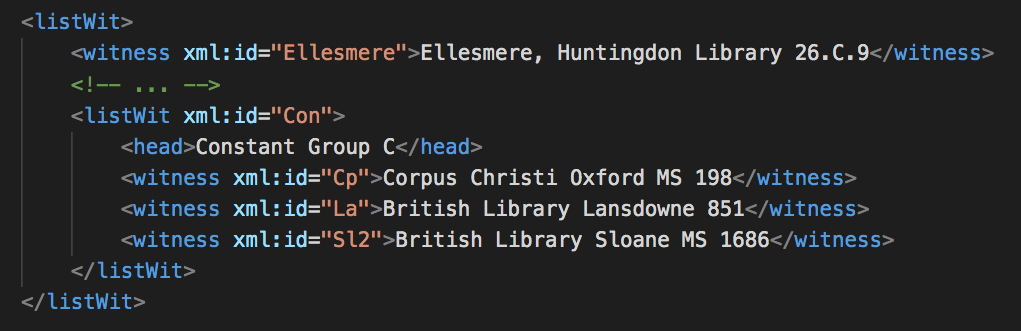
\includegraphics[width=.95\textwidth]{imgs/listWit-nest.png}
       Le linee guida della TEI definiscono alcuni elementi per registrare in apparato testimoni frammentari
    \end{block}

    \begin{block}{Testimoni frammentari}
        all'interno di elementi \texttt{lem} oppure elementi \texttt{rdg} si può registrare l'inizio o la fine di un testimone frammentario ovvero l'inizio o la fine di una lacuna
     \end{block}


\end{frame}

\begin{frame}
    \frametitle{TEI Modulo 12 - Codifica Edizioni Critiche}
    \framesubtitle{Informazioni sui testimoni}
    \addtocounter{nframe}{1}

    
    \begin{block}{Testimoni frammentari}
       % 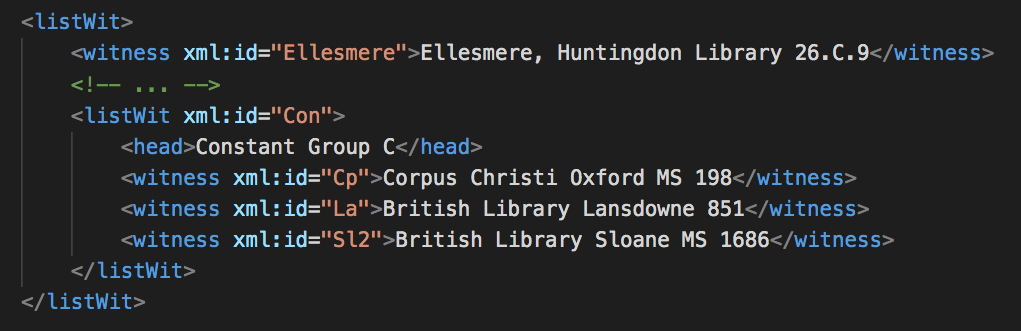
\includegraphics[width=.95\textwidth]{imgs/listWit-nest.png}

       \begin{itemize}
           \item \texttt{<witStart>} \textit{(fragmented witness start)} - indicates the beginning, or resumption, of the text of a fragmentary witness.
           \item \texttt{<witEnd>} \textit{(fragmented witness end)} -  indicates the end, or suspension, of the text of a fragmentary witness.
           \item \texttt{<lacunaStart>} indicates the beginning of a lacuna in the text of a mostly complete textual witness.
           \item \texttt{<lacunaEnd>} indicates the end of a lacuna in a mostly complete textual witness.
       \end{itemize}
      
    \end{block}


\end{frame}



\begin{frame}
    \frametitle{TEI Modulo 12 - Codifica Edizioni Critiche}
    \framesubtitle{Informazioni sui testimoni}
    \addtocounter{nframe}{1}
    
    % * Evidenziazione, page 16
    % In an apparatus this might appear thus, distinguished from the reading of other manuscripts by the presence of the lacunaEnd element:

    % * Evidenziazione, page 16
    % <app> <lem wit="#El #Hg">Auctoritee</lem> <rdg wit="#La #Ra2">auctorite</rdg> <rdg wit="#X"> <lacunaEnd/>auctorite</rdg> </app>

    % * Evidenziazione, page 16
    % <app> <lem wit="#El #Hg">Auctoritee</lem> <rdg wit="#La #Ra2 #X"> <lacunaEnd wit="#X"/>auctorite</rdg> </app>

    % * Evidenziazione, page 16
    % In some cases, the apparatus in the source may commence recording the readings for a particular witness without its being clear whether the previous absence of readings for this witness is due to a lacuna

    % * Evidenziazione, page 16
    % The witStart element may be used in this circumstance:

    % * Evidenziazione, page 16
    % <app> <lem wit="#El #Hg">Auctoritee</lem> <rdg wit="#La #Ra2">auctorite</rdg> <rdg wit="#X"> <witStart/>auctorite</rdg> </app>

    \begin{block}{Testimoni frammentari}
       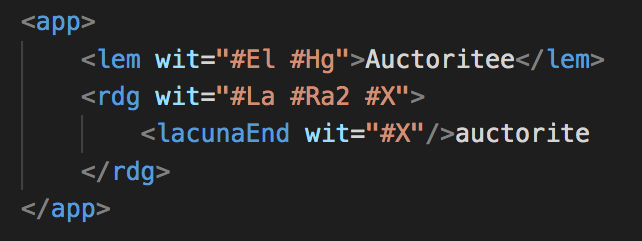
\includegraphics[width=.95\textwidth]{imgs/rdg-lacunaEnd.png}
    \end{block}

    \begin{block}{Testimoni frammentari}
        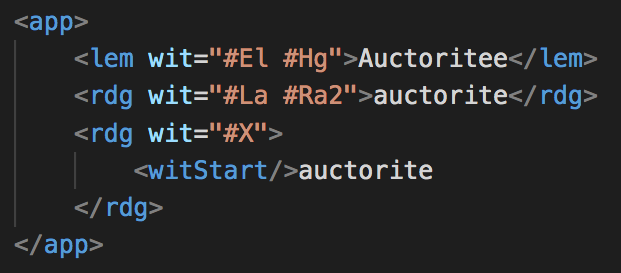
\includegraphics[width=.95\textwidth]{imgs/rdg-witStart.png}
     \end{block}


\end{frame}


\begin{frame}
    \frametitle{TEI Modulo 12 - Codifica Edizioni Critiche}
    \framesubtitle{link a critical apparatus to the text:}
    \addtocounter{nframe}{1}
    
    % * Evidenziazione, page 16
    % the location-referenced method,

    % * Evidenziazione, page 16
    % the double-end-point-attached method

    % * Evidenziazione, page 16
    % the parallel segmentation method

    
    \begin{block}{Three different methods}
       \begin{itemize}
           \item the location-referenced method
           \item the double-end-point-attached method
           \item the parallel segmentation method
       \end{itemize}
     \end{block}


\end{frame}


\begin{frame}
    \frametitle{TEI Modulo 12 - Codifica Edizioni Critiche}
    \framesubtitle{link a critical apparatus to the text}
    \addtocounter{nframe}{1}
    
    \begin{block}{Three different methods}
       \begin{itemize}
           \item in-line or external apparatus
           \begin{itemize}
             \item All'interno oppure esternamente al documento che registra il testo di base
             \item location-referenced & double-end-point-attached
           \end{itemize}
           \item  parallel segmentation method
            \begin{itemize}
                \item non ha il concetto di "testo base"
                \item codifica solo in-line
            \end{itemize}
       \end{itemize}
     \end{block}

\end{frame}

\begin{frame}
    \frametitle{TEI Modulo 12 - Codifica Edizioni Critiche}
    \framesubtitle{link a critical apparatus to the text}
    \addtocounter{nframe}{1}

    % * Evidenziazione, page 16
    % the location-referenced and the double end-point methods may be used with either in-line or external apparatus

    % * Evidenziazione, page 16
    % former dispersed within the base text

    % * Evidenziazione, page 16
    % latter held in some separate

    % * Nota ancorata, page 16
    % Ci si riferisce al metodo inline

    % Ci si riferisce al metodo inline

    % * Evidenziazione, page 17
    % location

    % * Evidenziazione, page 17
    % within or outside the document with the base text

    % * Evidenziazione, page 17
    % The parallel segmentation method does not use the concept of a base text and may only be used for in-line apparatus
    
    \begin{block}{Three different methods}
       \begin{itemize}
           \item in-line or external apparatus
           \begin{itemize}
             \item All'interno oppure esternamente al documento che registra il testo di base
             \item location-referenced & double-end-point-attached
           \end{itemize}
           \item  parallel segmentation method
            \begin{itemize}
                \item non ha il concetto di "testo base"
                \item codifica solo in-line
            \end{itemize}
       \end{itemize}
     \end{block}

\end{frame}



\begin{frame}
    \frametitle{TEI Modulo 12 - Codifica Edizioni Critiche}
    \framesubtitle{link a critical apparatus to the text}
    \addtocounter{nframe}{1}
  
    \begin{block}{Three different methods}
       \begin{itemize}
           \item external apparatus
           \begin{itemize}
             \item \texttt{<listApp>} \textit{(list of apparatus entries)} - contains a list of apparatus entries. att.typed provides attributes which can be used to classify or subclassify elements in any way.
             \item \texttt{@type} - characterizes the element in some sense, using any convenient classification scheme or typology
             \item \texttt{@subtype} - provides a sub-categorization of the element, if needed
           \end{itemize}
       \end{itemize}
     \end{block}

\end{frame}


\begin{frame}
    \frametitle{TEI Modulo 12 - Codifica Edizioni Critiche}
    \framesubtitle{link a critical apparatus to the text}
    \addtocounter{nframe}{1}
  
    % * Evidenziazione, page 17
    % Any document containing app elements requires a variantEncoding declaration in the encodingDesc element of its TEI heade

    % * Evidenziazione, page 17
    % <variantEncoding> declares the method used to encode text-critical variants.

    % * Evidenziazione, page 17
    % @method

    % * Evidenziazione, page 17
    % @location

    % * Evidenziazione, page 17
    % appears within the running text or external

    \begin{block}{Three different methods}
       \begin{itemize}
           \item Ciascun documento che presenta un elemento app richiede di dichiarare nell'intestazione del documento il metodo utilizzato per la codifica dell'apparato critico
           \begin{itemize}
             \item <variantEncoding> declares the method used to encode text-critical variants.
             \item @method indicates which method is used to encode the apparatus of variants.
             \item @location indicates whether the apparatus appears within the running text or external to it.
           \end{itemize}
       \end{itemize}
     \end{block}

\end{frame}

%% ESEMPIO

\begin{frame}
    \frametitle{TEI Modulo 12 - Codifica Edizioni Critiche}
    \framesubtitle{link a critical apparatus to the text}
    \addtocounter{nframe}{1}
    

    \begin{center}
       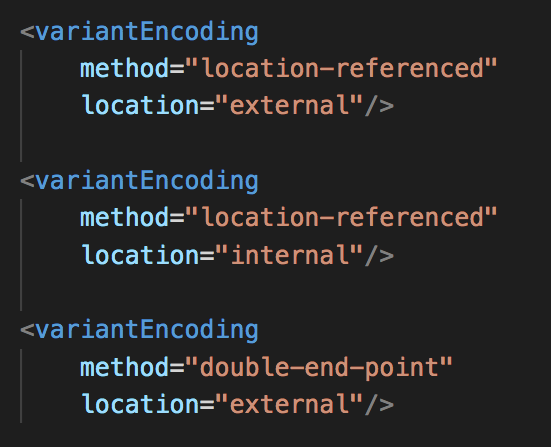
\includegraphics[width=.95\textwidth]{imgs/variantEncoding.png}
    \end{center}

\end{frame}



\begin{frame}
    \frametitle{TEI Modulo 12 - Codifica Edizioni Critiche}
    \framesubtitle{location-referenced method}
    \addtocounter{nframe}{1}
    

    \begin{center}
       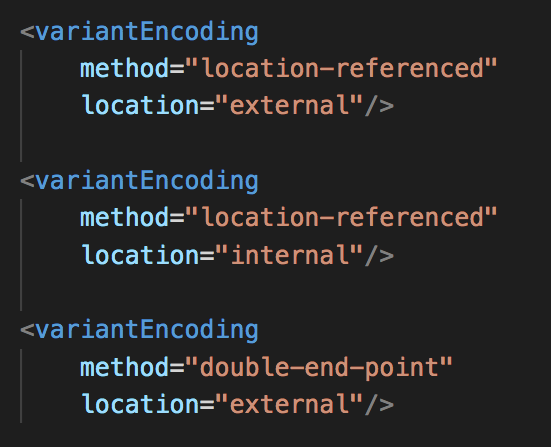
\includegraphics[width=.95\textwidth]{imgs/variantEncoding.png}
    \end{center}

\end{frame}




% * Evidenziazione, page 17
% The location-referenced method of encoding apparatus provides a convenient method for encoding printed apparatus

% * Evidenziazione, page 17
% the apparatus is linked to the base text by indicating explicitly only the block of text on which there is a variant

% * Evidenziazione, page 17
% usually by a canonical reference scheme, or by line number in the edition

% * Evidenziazione, page 17
% If the location-referenced method is used for an apparatus stored externally to the base text, the TEI header must have the declaration

% * Evidenziazione, page 17
% <variantEncoding method="location-referenced" location="external"/>

% * Evidenziazione, page 17
% In the body of the document, the base text (here El) will appear

% * Evidenziazione, page 18
% Elsewhere in the document, or in a separate file, the apparatus will appear

% * Evidenziazione, page 18
% On each app element, the @loc attribute should be specified to indicate where the variant occurs in the base text.

% * Evidenziazione, page 18
% <app loc="WBP 1"> <rdg wit="#La">Experiment</rdg> <rdg wit="#Ra2">Eryment</rdg> </app>

% * Evidenziazione, page 18
% encoded using in-line storage

% * Evidenziazione, page 18
% apparatus is dispersed through the base text block to which it refers

% * Evidenziazione, page 18
% In this case, the location of the variant can be read from the line in which it occurs

% * Evidenziazione, page 18
% <variantEncoding method="location-referenced" location="internal"/>

% * Nota ancorata, page 18
% in-line location referenced method

% Quando si registrano le varianti inline, il testo base va riportato fuori dall'apparato

% * Evidenziazione, page 18
% Since the location is not required to be exact, the apparatus for a line might also appear at the end of the line:

% * Evidenziazione, page 18
% <l n="1">Experience though noon Auctoritee <app> <rdg wit="#La"> Experiment</rdg> <rdg wit="#Ra2"> Eryment</rdg> </app> </l>

% * Evidenziazione, page 18
% it is not possible to find automatically the precise portion of text varied by the readings

% * Evidenziazione, page 18
% In order to show explicitly what portion of the base text is replaced by the variant readings, the lem element may be used:

% * Evidenziazione, page 19
% no recommendations are made for conventions of abbreviating the lemma

% * Evidenziazione, page 19
% simple location-reference methods are unlikely to be as successful as the other two methods, which allow the unambiguous reconstruction of the lemma from the encoding.



\begin{frame}
    \frametitle{TEI Modulo 12 - Codifica Edizioni Critiche}
    \framesubtitle{double end-point attachment method}
    \addtocounter{nframe}{1}
    

    \begin{center}
       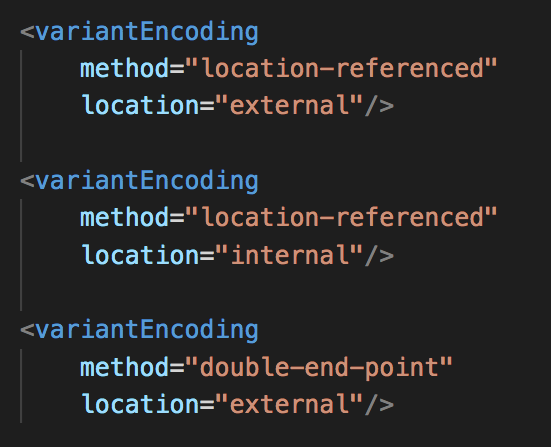
\includegraphics[width=.95\textwidth]{imgs/variantEncoding.png}
    \end{center}

\end{frame}




% * Evidenziazione, page 19
% In the double end-point attachment method, the beginning and end of the lemma in the base text are both explicitly indicated

% * Evidenziazione, page 19
% Double end-point attachment permits unambiguous matching of each variant reading against its lemma

% * Evidenziazione, page 19
% where the apparatus is intended to enable full reconstruction of the text

% * Evidenziazione, page 19
% the @from and @to attributes of the app element are used to indicate the beginning and ending points of the reading in the base text:

% * Evidenziazione, page 19
% identifiers which occur at the locations in question

% * Evidenziazione, page 19
% If no other markup is present there, the beginning and ending points should be marked using the anchor element

% * Evidenziazione, page 19
% he beginning and end of the lemma may be indicated by using the ‘indirect pointing’ mechanisms

% * Evidenziazione, page 19
% The double end-point attachment method may be used with in-line or external apparatus

% * Evidenziazione, page 19
% the base text (here El) will appear with anchor elements inserted at every place where a variant begins or ends

% * Evidenziazione, page 19
% unless some element with an identifier already begins or ends at that point

% * Evidenziazione, page 19
% <variantEncoding method="double-end-point" location="external"/> <!-- ... --> <div n="WBP" type="prologue"> <head>The Prologe ... </head> <l n="1" xml:id="WBP.1">Experience<anchor xml:id="WBP-A2"/> though noon Auctoritee</l> <l>Were in this world ...</l> </div>

% * Evidenziazione, page 19
% separately encoded

% * Evidenziazione, page 19
% <app from="#WBP.1" to="#WBP-A2"> <rdg wit="#La">Experiment</rdg>

% * Evidenziazione, page 20
% <rdg wit="#Ra2">Eryment</rdg> </app>

% * Evidenziazione, page 20
% No anchor element is needed at the beginning of the line, since the @from attribute can use the identifier for the line as a whole

% * Evidenziazione, page 20
% the lemma is assumed to run from the beginning of the element indicated by the @from attribute, to the end of that indicated by the @to attribute

% * Evidenziazione, page 20
% If no value is given for @to, the lemma runs from the beginning to the end of the element indicated by the @from attribute.

% * Evidenziazione, page 20
% When the apparatus is encoded in-line, it is dispersed through the base text

% * Evidenziazione, page 20
% Only the beginning of the lemma need be marked with an anchor, since the app is inserted at the end of the lemma, and itself therefore marks the end of the lemma.

% * Evidenziazione, page 20
% <variantEncoding method="double-end-point" location="internal"/> <!-- ... --> <l n="1" xml:id="wbp.1">Experience <app from="#wbp.1"> <rdg wit="#La">Experiment</rdg> <rdg wit="#Ra2">Eryment</rdg> </app> though noon Auctoritee</l> <l>Were in this world ...</l>

% * Evidenziazione, page 20
% The lemma need not be repeated within the app element in this method, as it may be extracted reliably from the base text

% * Evidenziazione, page 20
% if it is desired to make an explicit record of the attestation of the base text, the lem element may be embedded within app, carrying the witnesses to the base

% * Evidenziazione, page 20
% <app from="#WBP.1" to="#WBP-A2"> <lem wit="#El #Hg">Experience</lem>

% * Evidenziazione, page 20
% This method is designed to cope with ‘overlapping lemmata’

% * Evidenziazione, page 21
% This method can readily cope with such difficult situations

% * Evidenziazione, page 21
% typically found in large and complex traditions

% * Evidenziazione, page 21
% <l xml:id="WBP.117" n="117"> And <anchor xml:id="WBP-A117.1"/> of so parfit <anchor xml:id="WBP-A117.2"/> wys <anchor xml:id="WBP-A117.3"/> a wight <anchor xml:id="WBP-A117.4"/> ywroght

% * Evidenziazione, page 21
% <app from="#WBP-A117.1" to="#WBP-A117.3"> <lem wit="#Hg">of so parfit wys</lem> <rdg wit="#Ha4">in what wise was</rdg> </app>

% * Evidenziazione, page 21
% <app from="#WBP-A117.2" to="#WBP-A117.4"> <lem wit="#Hg">wys a wight</lem> <rdg wit="#El #Ha4">was a wight</rdg> </app>





\begin{frame}
    \frametitle{TEI Modulo 12 - Codifica Edizioni Critiche}
    \framesubtitle{parallel segmentation method}
    \addtocounter{nframe}{1}
    

    \begin{center}
       \includegraphics[width=.95\textwidth]{imgs/variantEncoding.png}
    \end{center}

\end{frame}






% * Evidenziazione, page 21
% The parallel segmentation method, to be discussed next, cannot handle overlaps among variants

% * Evidenziazione, page 21
% This method differs from the double end-point attachment method in that all variants at any point of the text are expressed as variants on one another.

% * Evidenziazione, page 21
% In this method, no two variations can overlap, although they may nest

% * Evidenziazione, page 21
% The texts compared are divided into matching segments all synchronized with one another

% * Evidenziazione, page 21
% It is also very easy with this method for an application to extract the full text of any one witness from the apparatus

% * Evidenziazione, page 21
% It will however be less convenient for very complex traditions

% * Evidenziazione, page 21
% In the parallel segmentation method, each segment of text on which there is variation is marked by an app element

% * Evidenziazione, page 21
% If there is a preferred (or base) reading it is tagged with lem; each reading is given in a rdg element:

% * Evidenziazione, page 22
% This method cannot be used with external apparatus

% * Evidenziazione, page 22
% it must be used in-line

% * Evidenziazione, page 22
% the witnesses to the reading most widely attested need not be stated

% * Evidenziazione, page 22
% read a listWit declaring all the witnesses to the text and then calculate which witnesses have not been named

% * Evidenziazione, page 22
% To avoid confusion, however, witnesses may be omitted only for a single reading.

% * Evidenziazione, page 22
% <l n="1"> <app> <lem>Experience</lem> <rdg wit="#La">Experiment</rdg> <rdg wit="#Ra2">Eryment</rdg> </app> though noon Auctoritee </l>

% * Evidenziazione, page 22
% apparatus entries may nest in this method

% * Evidenziazione, page 22
% the variation on the individual words of the line would nest within that for the line as a whole:

% * Evidenziazione, page 22
% <rdg wit="#Chi3">Auctoritee, though none experience</rdg> <rdg> <app> <rdg wit="#El #Hg">Experience</rdg> <rdg wit="#La">Experiment</rdg> <rdg wit="#Ra2">Eryment</rdg> </app> <app> <rdg wit="#El #Ra2">though</rdg> <rdg wit="#Hg">thogh</rdg> <rdg wit="#La">thouh</rdg> </app> <app> <rdg wit="#El #Hg">noon Auctorite</rdg> <rdg wit="#La #Ra2">none auctorite</rdg> </app> </rdg>

% * Evidenziazione, page 23
% Parallel segmentation cannot, however, deal very gracefully with variants which overlap without nesting




\begin{frame}
    \frametitle{TEI Modulo 12 - Codifica Edizioni Critiche}
    \framesubtitle{}
    \addtocounter{nframe}{1}
    

    \begin{center}
       \includegraphics[width=.95\textwidth]{imgs/variantEncoding.png}
    \end{center}

\end{frame}





% * Evidenziazione, page 23
% When an apparatus is provided it does not need to be given at the location in the transcription where the variation, emendation, attribution, or other apparatus observation occurs. Instead it may be stored in a separate place in the same file, or indeed in another file, and point to the location at which it is meant to be used

% * Evidenziazione, page 23
% The location-referenced method can be used to point a position in a text using the @loc attribute and a canonical reference that is understood and documented in the context of the file where it is used

% * Evidenziazione, page 23
% Where possible it is recommended that other methods use the @from attribute to point to an @xml:id attribute on an anchor or other element at the location where the apparatus observation takes place

% * Evidenziazione, page 23
% The contents of an element pointed to are understood to be equivalent to a lem if none exists in the app, and if a lem does exist this should replace any content.

% * Evidenziazione, page 23
% The @from attribute is a data.pointer datatype and thus contains a URI as a value

% * Evidenziazione, page 23
% directly to an @xml:id, an @xml:id in another local file, or indeed a file identified by any URL or URN

% * Evidenziazione, page 23
% <app from="example.xml#WBP-so.1.1">

% * Evidenziazione, page 23
% could also be encoded as

% * Evidenziazione, page 23
% <anchor xml:id="WBP-so.1.1a"/>

% * Evidenziazione, page 23
% <app from="http://www.example.com/example.xml#WBP-so.1.1a"> <lem>Experience</lem>

% * Evidenziazione, page 24
% In addition, URLs can contain XPointer schemes including xpath(), range(), and string-range() which can be used in providing the location of an app that is stored separately from the text to which it applies

% * Evidenziazione, page 24
% Both @from and @to can be used, as in the double end-point attachment method, to identify the starting and ending location for an apparatus using XPointer schemes described

% * Evidenziazione, page 24
% <l n="1" xml:id="WP.1a">Experience though noon Auctoritee</l>

% * Evidenziazione, page 24
% <app from="example.xml#string-range(WP.1a, 0, 10)"> <lem>Experience</lem>

% * Evidenziazione, page 24
% If only the @from attribute is provided then it should be understood that this supplies the location of the textual variance that the apparatus documents

% * Evidenziazione, page 24
% If the @from attribute contains an XPointer scheme that identifies a range of text

% * Evidenziazione, page 24
% record the starting and ending of the range

% * Evidenziazione, page 24
% In such a case a @to attribute is unnecessary.




\begin{frame}
    \frametitle{TEI Modulo 12 - Codifica Edizioni Critiche}
    \framesubtitle{record different transcriptions}
    \addtocounter{nframe}{1}
    

    \begin{center}
       \includegraphics[width=.95\textwidth]{imgs/variantEncoding.png}
    \end{center}

\end{frame}



% * Evidenziazione, page 24
% It is often desirable to record different transcriptions of one stretch of text.

% * Evidenziazione, page 24
% An application may then construct different ‘views’ of the transcription by extraction of the appropriate variant readings from the apparatus elements embedded in the transcription.

% * Evidenziazione, page 24
% For example, alternative expansions can be recorded in several different expan elements, all grouped within an app element

% * Evidenziazione, page 24
% which has been read in different ways by different scholars

% * Evidenziazione, page 24
% This information may be held within an app structure

% * Evidenziazione, page 24
% <app> <rdg source="#ES">perfectio<am> <g ref="#ii"/> </am> </rdg> <rdg source="#FJF">perfectio<ex>u</ex>n</rdg> <rdg source="#PGR">perfectiou<ex>n</ex>

% * Evidenziazione, page 25
% Editorial notes may also be attached to app structures within transcriptions

% * Evidenziazione, page 25
% In most cases, elements used to indicate features of a primary textual source may be represented within an app structure simply by nesting them within its readings

% * Evidenziazione, page 25
% the markup may use the join element or the @next and @prev attributes defined by chapter





\begin{frame}
    \frametitle{TEI Modulo 12 - Codifica Edizioni Critiche}
    \framesubtitle{Strategies for Encoding Variation}
    \addtocounter{nframe}{1}
    

    \begin{center}
       \includegraphics[width=.95\textwidth]{imgs/variantEncoding.png}
    \end{center}

\end{frame}





% * Evidenziazione, page 25
% Variation most frequently occurs at the phrase level, but is also common at higher structural levels, such as the verse line, paragraph, or chapter

% * Evidenziazione, page 25
% some care must be taken in their encoding to ensure that TEI's Abstract Model is not being broken.

% * Evidenziazione, page 26
% Similarly, it is an error if the contents of an apparatus entry place a p inside another p or an l inside an l.

% * Evidenziazione, page 26
% Phenomena such as omissions and transpositions in witnesses will require some encoding strategies that differ from those in the examples above

% * Evidenziazione, page 26
% An editor wishing to signal an omission in one witness should encode the omission using an empty rdg

% * Evidenziazione, page 26
% <app xml:id="d1e372"> <lem xml:id="d1e373" source="#Heyworth"> <l n="18">Hypsipyle uacuo constitit in thalamo:</l> </lem> <rdg xml:id="d1e376" wit="#J" cause="homeoarchon"/> </app>

% * Evidenziazione, page 26
% Notice that in this example, the variation occurs at the unit of the verse line

% * Evidenziazione, page 26
% by mistake

% * Evidenziazione, page 26
% If a witness contains an interpolation that the editor does not wish to show in the base text, an empty lem should be used, in the same fashion.

% * Evidenziazione, page 26
% Transpositions are harder to encode

% * Evidenziazione, page 26
% A single app will therefore not be sufficient

% * Evidenziazione, page 26
% and the variants must be linked.

% * Evidenziazione, page 26
% <app xml:id="app-lem-l25-l26" exclude="#app-rdg-Housman-l25-26"> <lem xml:id="d1e462" source="#Heyworth"> <l n="25" xml:id="l25">desine iam reuocare tuis periuria verbis,</l> <l n="26" xml:id="l26">Cynthia, et oblitos parce movere deos;</l> </lem> </app>

% * Evidenziazione, page 26
% <app xml:id="app-rdg-Housman-l25-26" exclude="#app-lem-l25-l26"> <rdg xml:id="d1e603" source="#Housman"> <l copyOf="#l25"/> <l copyOf="#l26"/> </rdg> <note target="#d1e603">Housman put these lines after 32.</note> </app>

% * Evidenziazione, page 26
% Note that both apps are linked via the @exclude attribut

% * Evidenziazione, page 26
% because they are mutually exclusive

% * Evidenziazione, page 26
% To avoid repetition, the second pair of lines can make use of the @copyOf attribute.

% * Evidenziazione, page 26
% Apparatus entries may nest when there is variation at both higher and lower structural levels

% * Evidenziazione, page 27
% <app xml:id="d1e275"> <lem xml:id="d1e277" source="#Heyworth"> <l n="8"> <app xml:id="d1e280"> <lem xml:id="d1e281" wit="#N #Λ">ut</lem> <rdg xml:id="d1e283" wit="#A">et</rdg> <rdg xml:id="d1e285" source="#Nodell">ac</rdg> <note target="#d1e287">perhaps</note> <rdg xml:id="d1e287" source="#Heyworth" cert="low">quam</rdg> </app> formosa nouo quae parat ire uiro.</l> <l n="9"> <app xml:id="d1e294"> <lem xml:id="d1e295">at</lem> <rdg xml:id="d1e297" wit="#A">et</rdg> </app> non sic, Ithaci digressu <app xml:id="d1e300"> <lem xml:id="d1e301">mota</lem> <rdg xml:id="d1e303" source="#Graevius">immota</rdg> </app>, Calypso</l> <l n="10">desertis olim fleuerat aequoribus:</l> <l n="11">multos illa dies incomptis maesta capillis</l> </lem> <rdg xml:id="d1e314" wit="#C" cause="homoeoteleuton"/> <note target="#d1e314">omits lines 8-11 because of homoeoteleuton.</note> </app>

% * Evidenziazione, page 27
% Here, MS C omits lines 8-11, but there are variations the editor wishes to record in the other witnesses which do have these lines

% * Evidenziazione, page 27
% Therefore, an outer app gives the lines in the lem and the omission in a rdg

% * Evidenziazione, page 27
% Further variation is encoded for lines 8 and 9 using nested apps.





% This panel addresses the TEI critical apparatus as a data model, investigating how it has expanded the capacity of scholarly editions to articulate and analyze phenomena of textual variation and multiplicity. We will discuss how the TEI critical apparatus, as a structure that mediates distinct versions of a work, is expanding horizons for multidimensional and pluralistic document modeling. Our panel surveys recent experiments with the critical apparatus that have led to new kinds of scholarly research and in some cases to revisions to the TEI Guidelines. What kinds of research questions and applications can we support with the TEI critical apparatus, and what practical challenges do we face in working with it in inline and stand-off ways? We begin by investigating how the TEI critical apparatus has transformed the expressive capacity of scholarly editions to prioritize textual multiplicity. We continue by sharing data models that apply TEI critical apparatus as a stand-off “spine” for connecting independently encoded witnesses. We conclude by inviting the audience to discuss with us the scalability of these methods for texts with large numbers of witnesses, and the technological challenges and opportunities of stand-off methods in light of recent changes to the TEI Guidelines. 

% What *really* is a critical apparatus (James Cummings)

\section{Strumenti per edizioni critiche}
% - Tool di allineamento per la collazione:
%
% -- http://v-machine.org/documentation/
%
% -- https://collatex.net/
%
% -- http://www.juxtacommons.org/
%
% -- https://sada.uzi.uni-halle.de/
%
% -- medite
%
% -- tustep/TXSTEP
%
% -- stemmaWeb
%
% -- Classical Text Editor
%
% -- http://evt.labcd.unipi.it/

% -- http://www.informatik.uni-leipzig.de:8080/BibleViz/
% -- http://www.traviz.vizcovery.org/examples.html

% ecdotica: resa grafica, messa in pagina
% -- https://ride.i-d-e.de/issues/issue-11/reledmac/
% -- https://tei-c.org/2014/06/10/tei-critical-edition-toolbox/
% -- http://teicat.huma-num.fr/index.php

% Could be utilized to divide the process into an automated collation layer and a human interpretation layer.

\begin{frame}
	\frametitle{Strumenti per edizioni critiche}
	\addtocounter{nframe}{1}
    \begin{block}{Preparazione}
        %  a philologist consults an immense number of copies and related sources while engaging in the study of the history of one text;
        % identify the differences between witnesses
        % variant readings are often encoded manually by human editors
        % automatic text collation
        % adaptable tools which can handle textual variance and text alignment
        % support for TEI-XML markup
        % stemma codicum
	\end{block}
	\begin{block}{Visualizzazione}
       % There are various conventional methods to present the results of a given text collation in printed editions
       % classical scholarly editions prefer a critical apparatus: one witness or the established critical text is chosen as base-text, while all variants are presented in footnotes or endnotes
       % A more visual presentation mode is synopsis: all collated texts are presented in parallel, either in vertical or horizontal order
       % digital tools can also help to create presentations dynamically
       % The creation of user-configurable visualizations is supported by a basic digital paradigm: separating the visual presentation (e.g. HTML) from the encoded
	\end{block}
\end{frame}

%  Changes are catalogued in a critical apparatus
        % A typical entry starts with the variant’s position (usually line or paragraph number), followed by the lemma of the base text often delimited by a closing square bracket ‘]’
        % follows the variant text itself and finally the corresponding sigla of the sources

\begin{frame}
	\frametitle{Philological computational tools}
	\addtocounter{nframe}{1}
    \begin{block}{Collation tools}
            
		\begin{block}
			% interest in retracing the creation and transmission of texts in order to establish connections or divergences between them
            % collation tools: Juxta Web Service1, LERA2, and Variance Viewer
            % philological text collation tool needs to build a bridge between technical and scholarly understanding
            % Collating long texts turned out to be a complex scenario
            % 2009, a working group presented an abstract framework for complex text collation procedures, which was later called ‘Gothenburg mode
            % five different computing stages (tokenization, normalization, alignment, analysis, and visualization). Nassourou (2013) proposed to extend this model by a sixth, interpretative layer
		\end{block}
	\end{block}
\end{frame}

\begin{frame}
	\frametitle{Philological computational tools}
	\addtocounter{nframe}{1}
    \begin{block}{Collation tools}
		\begin{itemize}
			\item CollateX
			\item Variance Viewer
			\item Juxta Web Service
			\item StemmaWeb
			\item TUSTEP/TXSTEP
			\item MEDITE
		\end{itemize}
	\end{block}
\end{frame}

\begin{frame}
	\frametitle{Philological computational tools}
	\addtocounter{nframe}{1}
    \begin{block}{Visualization/Publication tools}
		\begin{itemize}
			\item Classical Text Editor (CTE)
			\item TEIpublisher
			\item Edition Visualization Technology (EVT)
			\item TextualCommunities
			\item Versioning Machine
			\item LERA/SADA project
			\item Critical Edition Toolbox
			\item LaTex/Reledmac
			\item TRAVIZ/ITEAL
			\item EUPORIA
		\end{itemize}
	\end{block}
\end{frame}

% Stemma: si definisce stemma codicum o albero genealogico, la rappresentazione grafica dei rapporti genetici fra i testimoni, ricostruiti attraverso la rilevazione e la valutazione degli errori (vd.) di cui ciascuno è portatore.


\begin{frame}
    \frametitle{Strumenti per edizioni critiche}
    \framesubtitle{Strumenti di collazione automatica}
	\addtocounter{nframe}{1}
    \begin{center}
        \textbf{CollateX}
    \end{center}
    \begin{center}
        \textit{\url{https://collatex.net}}
	\end{center}
    \begin{center}
        \includegraphics[width=.95\textwidth]{imgs/collatex.png}
	\end{center}
\end{frame}

\begin{frame}
    \frametitle{Strumenti per edizioni critiche}
    \framesubtitle{Strumenti di collazione automatica}
	\addtocounter{nframe}{1}
    \begin{center}
        \textbf{Variance Viewer}
    \end{center}
    \begin{center}
        \textit{\url{http://variance-viewer.informatik.uni-wuerzburg.de/Variance-Viewer/}}
	\end{center}
    \begin{center}
        \includegraphics[width=.95\textwidth]{imgs/variance-viewer.png}
	\end{center}
\end{frame}

\begin{frame}
    \frametitle{Strumenti per edizioni critiche}
    \framesubtitle{Strumenti di collazione automatica}
	\addtocounter{nframe}{1}
    \begin{center}
        \textbf{Juxta Web Service}
    \end{center}
    \begin{center}
        \textit{\url{http://juxtacommons.org/}}
	\end{center}
    \begin{center}
        \includegraphics[width=.95\textwidth]{imgs/juxtaweb.png}
	\end{center}
\end{frame}

\begin{frame}
    \frametitle{Strumenti per edizioni critiche}
    \framesubtitle{Strumenti di collazione automatica}
	\addtocounter{nframe}{1}
    \begin{center}
        \textbf{StemmaWeb}
    \end{center}
    \begin{center}
        \textit{\url{https://stemmaweb.net/stemmaweb/}}
	\end{center}
    \begin{center}
        \includegraphics[width=.95\textwidth]{imgs/}
	\end{center}
\end{frame}

\begin{frame}
    \frametitle{Strumenti per edizioni critiche}
    \framesubtitle{Strumenti di collazione automatica}
	\addtocounter{nframe}{1}
    \begin{center}
        \textbf{TUebingen System of Text Processing Programs" TUSTEP - TXSTEP}
    \end{center}
    \begin{center}
        \textit{\url{https://www.tustep.uni-tuebingen.de/tustep_eng.html}}
	\end{center}
    \begin{center}
        %\includegraphics[width=.95\textwidth]{imgs/}
        TODO
	\end{center}
\end{frame}

\begin{frame}
    \frametitle{Strumenti per edizioni critiche}
    \framesubtitle{Strumenti di collazione automatica}
	\addtocounter{nframe}{1}
    \begin{center}
        \textbf{MEDITE}
    \end{center}
    \begin{center}
        \textit{\url{http://www-poleia.lip6.fr/~ganascia/Medite_Project}}
	\end{center}
    \begin{center}
        \includegraphics[width=.95\textwidth]{imgs/tustep.jpg}
	\end{center}
\end{frame}




\begin{frame}
    \frametitle{Strumenti per edizioni critiche}
    \framesubtitle{Strumenti per la visualizzazione e pubblicazione}
	\addtocounter{nframe}{1}
    \begin{center}
        \textbf{Classical Text Editor}
    \end{center}
    \begin{center}
        \textit{\url{https://cte.oeaw.ac.at/}}
	\end{center}
    \begin{center}
        \includegraphics[width=.95\textwidth]{imgs/cte.gif}
	\end{center}
\end{frame}

\begin{frame}
    \frametitle{Strumenti per edizioni critiche}
    \framesubtitle{Strumenti per la visualizzazione e pubblicazione}
	\addtocounter{nframe}{1}
    \begin{center}
        \textbf{TEIpublisher}
    \end{center}
    \begin{center}
        \textit{\url{https://teipublisher.com/index.html}}
	\end{center}
    \begin{center}
        \includegraphics[width=.95\textwidth]{imgs/teipublisher.png}
	\end{center}
\end{frame}

\begin{frame}
    \frametitle{Strumenti per edizioni critiche}
    \framesubtitle{Strumenti per la visualizzazione e pubblicazione}
	\addtocounter{nframe}{1}
    \begin{center}
        \textbf{Edition Visualization Technology (EVT)}
    \end{center}
    \begin{center}
        \textit{\url{http://evt.labcd.unipi.it}}
	\end{center}
    \begin{center}
        \includegraphics[width=.95\textwidth]{imgs/evt.png}
	\end{center}
\end{frame}

\begin{frame}
    \frametitle{Strumenti per edizioni critiche}
    \framesubtitle{Strumenti per la visualizzazione e pubblicazione}
	\addtocounter{nframe}{1}
    \begin{center}
        \textbf{Textual Communities}
    \end{center}
    \begin{center}
        \textit{\url{https://textualcommunities.org/app/}}
	\end{center}
    \begin{center}
        \includegraphics[width=.95\textwidth]{imgs/textualcommunities.png}
        
	\end{center}
\end{frame}

\begin{frame}
    \frametitle{Strumenti per edizioni critiche}
    \framesubtitle{Strumenti per la visualizzazione e pubblicazione}
	\addtocounter{nframe}{1}
    \begin{center}
        \textbf{Versioning Machine}
    \end{center}
    \begin{center}
        \textit{\url{http://v-machine.org}}
	\end{center}
    \begin{center}
        \includegraphics[width=.95\textwidth]{imgs/v-machine.png}
	\end{center}
\end{frame}

\begin{frame}
    \frametitle{Strumenti per edizioni critiche}
    \framesubtitle{Strumenti per la visualizzazione e pubblicazione}
	\addtocounter{nframe}{1}
    \begin{center}
        \textbf{LERA/SADA project}
    \end{center}
    \begin{center}
        \textit{\url{https://sada.uzi.uni-halle.de/}}
	\end{center}
    \begin{center}
        \includegraphics[width=.95\textwidth]{imgs/lara.png}
	\end{center}
\end{frame}

\begin{frame}
    \frametitle{Strumenti per edizioni critiche}
    \framesubtitle{Strumenti per la visualizzazione e pubblicazione}
	\addtocounter{nframe}{1}
    \begin{center}
        \textbf{Critical Edition Toolbox}
    \end{center}
    \begin{center}
        \textit{\url{http://teicat.huma-num.fr/index.php}}
	\end{center}
    \begin{center}
        \includegraphics[width=.95\textwidth]{imgs/}
	\end{center}
\end{frame}

\begin{frame}
    \frametitle{Strumenti per edizioni critiche}
    \framesubtitle{Strumenti per la visualizzazione e pubblicazione}
	\addtocounter{nframe}{1}
    \begin{center}
        \textbf{LaTex/Reledmac}
    \end{center}
    \begin{center}
        \textit{\url{https://ctan.org/pkg/reledmac}}
	\end{center}
    \begin{center}
        \includegraphics[width=.95\textwidth]{imgs/}
	\end{center}
\end{frame}

\begin{frame}
    \frametitle{Strumenti per edizioni critiche}
    \framesubtitle{Strumenti per la visualizzazione e pubblicazione}
	\addtocounter{nframe}{1}
    \begin{center}
        \textbf{TRAVIZ/ITEAL}
    \end{center}
    \begin{center}
        \textit{\url{http://www.traviz.vizcovery.org/}}
	\end{center}
    \begin{center}
        \includegraphics[width=.95\textwidth]{imgs/}
	\end{center}
\end{frame}

\begin{frame}
    \frametitle{Strumenti per edizioni critiche}
    \framesubtitle{Strumenti per la visualizzazione e pubblicazione}
	\addtocounter{nframe}{1}
    \begin{center}
        \textbf{EUPORIA}
    \end{center}
    \begin{center}
        \textit{cophilab.ilc.cnr.it}
	\end{center}
    \begin{center}
        \includegraphics[width=.95\textwidth]{imgs/}
	\end{center}
\end{frame}


\section{Considerazioni Finali}

% \begin{frame}
% 	\frametitle{Conclusion and Further Work}
% 	\addtocounter{nframe}{1}
% 	\begin{block}{Conclusion}
		
% 	\end{block}
% 	\begin{block}{Conclusion}
		
% 	\end{block}
% \end{frame}


% \begin{frame}
% 	\frametitle{Conclusion and Further Work}
% 	\addtocounter{nframe}{1}
% 	\begin{block}{Conclusion}
% 		\begin{itemize}
% 			\item 
% 			\item 
% 		\end{itemize}
% 	\end{block}
% \end{frame}


% \begin{frame}
% 	\frametitle{Conclusion and Further Work}
% 	\addtocounter{nframe}{1}
% 	\begin{block}{Conclusion:}
% 		\begin{itemize}
% 			\item<1-> 
% 			\item<2-> 
% 			\item<3-> 
% 			\item<4-> 
% 		\end{itemize}
% 	\end{block}
% \end{frame}

%% lavori futuri %%


\begin{frame}
	\frametitle{Conclusion and Further Work}
	\addtocounter{nframe}{1}
	\begin{block}{FINE DEL SEMINARIO!!}
		\begin{center}
			Grazie per la vostra paziente attenzione
		\end{center}
		\begin{center}
			\textbf{Se ci sono domande..}
		\end{center}
	\end{block}
\end{frame}



%\section{References}
%
%bibliografia
\begin{frame}
    \frametitle{References}
    \addtocounter{nframe}{1}
    \begin{thebibliography}{10}
    \end{thebibliography}

\end{frame}

\begin{frame}
    \frametitle{References}
    \addtocounter{nframe}{1}
    \begin{thebibliography}{10}
    \end{thebibliography}

\end{frame}


\end{document}